% =============================================================================
%  Βαθμονόμηση δύο σταδίων της διασπάσιμης κατάταξης ιστοσελίδων
%  Ελληνικό κείμενο (πλήρης μετάφραση του paper_en.tex).
%  Μεταγλώττιση:  xelatex paper_gr && xelatex paper_gr
%  Οι αριθμοί προέρχονται από το generated/macros.tex και οι πίνακες από το
%  generated/gr/, τα οποία γράφει το ../make_paper_assets.py από τα αποτελέσματα.
% =============================================================================
\documentclass[11pt,a4paper]{article}
\usepackage[a4paper,margin=2.3cm]{geometry}
\usepackage{amsmath,amssymb,amsthm}
\usepackage{txfonts}
\usepackage[no-math]{fontspec}
\setmainfont{FreeSerif}
\setmonofont{DejaVu Sans Mono}[Scale=0.82]
\usepackage[english,greek]{babel}
\renewcommand{\greekhyphenmins}{22}
\usepackage{graphicx}
\usepackage{booktabs}
\usepackage{array}
\usepackage[font=small,labelfont=bf]{caption}
\usepackage{enumitem}
\usepackage{algorithm}
\usepackage{algpseudocode}
\usepackage{microtype}
\usepackage{placeins}
\usepackage[hidelinks]{hyperref}

\newtheorem{theorem}{Θεώρημα}
\newtheorem{proposition}{Πρόταση}
\newtheorem{lemma}{Λήμμα}
\newtheorem{corollary}{Πόρισμα}
\theoremstyle{definition}
\newtheorem{definition}{Ορισμός}
\theoremstyle{remark}
\newtheorem{remark}{Παρατήρηση}

\addto\captionsgreek{\renewcommand{\refname}{Βιβλιογραφία}}
\floatname{algorithm}{Αλγόριθμος}
\algrenewcommand\algorithmicrequire{\textbf{Είσοδος:}}
\algrenewcommand\algorithmicrepeat{\textbf{επανάλαβε}}
\algrenewcommand\algorithmicuntil{\textbf{μέχρι}}
\algrenewcommand\algorithmicreturn{\textbf{επίστρεψε}}

% generated by make_paper_assets.py -- do not edit
% every value is mode-agnostic: signed numbers and powers of ten are wrapped in
% \ensuremath, so a macro can be used both in running text and inside $...$
\newcommand{\AnchorNcd}{0.852}
\newcommand{\AnchorNcdnf}{0.950}
\newcommand{\AnchorPop}{0.767}
\newcommand{\AnchorQ}{0.971}
\newcommand{\AnchorTot}{0.547}
\newcommand{\BoundCases}{\ensuremath{2\,948}}
\newcommand{\BoundGraphs}{14}
\newcommand{\BoundLoMax}{0.96}
\newcommand{\BoundLoMin}{0.94}
\newcommand{\BoundMax}{0.961}
\newcommand{\BoundMedEightyFive}{0.16}
\newcommand{\ConvNcdBound}{22.9}
\newcommand{\ConvNcdBoundK}{\ensuremath{85\to66}}
\newcommand{\ConvNcdReal}{13.1}
\newcommand{\ConvNcdTest}{14.7}
\newcommand{\ConvNfBound}{29.3}
\newcommand{\ConvNfBoundK}{\ensuremath{269\to190}}
\newcommand{\ConvNfReal}{15.3}
\newcommand{\ConvNfTest}{19.3}
\newcommand{\MaxSigmaDev}{\ensuremath{3.3\times10^{-16}}}
\newcommand{\MeanNcd}{0.791}
\newcommand{\MeanNcdnf}{0.914}
\newcommand{\MeanPop}{0.726}
\newcommand{\MeanQ}{0.968}
\newcommand{\MeanTot}{0.471}
\newcommand{\MisNcdNgHiCan}{\ensuremath{-0.0441}}
\newcommand{\MisNcdNgHiCanP}{\ensuremath{4.7\times10^{-10}}}
\newcommand{\MisNcdNgHiCanWins}{0/32}
\newcommand{\MisNcdNgHiNg}{\ensuremath{+0.0192}}
\newcommand{\MisNcdNgHiNgP}{\ensuremath{4.7\times10^{-10}}}
\newcommand{\MisNcdNgHiNgWins}{32/32}
\newcommand{\MisNcdRuleHiCan}{\ensuremath{-0.0414}}
\newcommand{\MisNcdRuleHiCanP}{\ensuremath{4.7\times10^{-10}}}
\newcommand{\MisNcdRuleHiCanWins}{0/32}
\newcommand{\MisNcdRuleHiNg}{\ensuremath{+0.0219}}
\newcommand{\MisNcdRuleHiNgP}{\ensuremath{1.5\times10^{-8}}}
\newcommand{\MisNcdRuleHiNgWins}{31/32}
\newcommand{\MisNcdRuleLoCan}{\ensuremath{+0.0110}}
\newcommand{\MisNcdRuleLoCanP}{\ensuremath{9.3\times10^{-10}}}
\newcommand{\MisNcdRuleLoCanWins}{31/32}
\newcommand{\MisNcdRuleLoNg}{\ensuremath{+0.0743}}
\newcommand{\MisNcdRuleLoNgP}{\ensuremath{4.7\times10^{-10}}}
\newcommand{\MisNcdRuleLoNgWins}{32/32}
\newcommand{\MisNcdnfNgHiCan}{\ensuremath{+0.0205}}
\newcommand{\MisNcdnfNgHiCanP}{\ensuremath{4.7\times10^{-10}}}
\newcommand{\MisNcdnfNgHiCanWins}{32/32}
\newcommand{\MisNcdnfNgHiNg}{\ensuremath{+0.0011}}
\newcommand{\MisNcdnfNgHiNgP}{0.062}
\newcommand{\MisNcdnfNgHiNgWins}{19/32}
\newcommand{\MisNcdnfRuleHiCan}{\ensuremath{+0.0283}}
\newcommand{\MisNcdnfRuleHiCanP}{\ensuremath{9.3\times10^{-10}}}
\newcommand{\MisNcdnfRuleHiCanWins}{31/32}
\newcommand{\MisNcdnfRuleHiNg}{\ensuremath{+0.0089}}
\newcommand{\MisNcdnfRuleHiNgP}{\ensuremath{5.0\times10^{-7}}}
\newcommand{\MisNcdnfRuleHiNgWins}{30/32}
\newcommand{\MisNcdnfRuleLoCan}{\ensuremath{-0.0109}}
\newcommand{\MisNcdnfRuleLoCanP}{\ensuremath{4.6\times10^{-6}}}
\newcommand{\MisNcdnfRuleLoCanWins}{6/32}
\newcommand{\MisNcdnfRuleLoNg}{\ensuremath{-0.0303}}
\newcommand{\MisNcdnfRuleLoNgP}{\ensuremath{4.7\times10^{-9}}}
\newcommand{\MisNcdnfRuleLoNgWins}{2/32}
\newcommand{\MisRuleBestCalib}{0.920}
\newcommand{\MisRuleBestCalibGap}{\ensuremath{+0.0002}}
\newcommand{\NfConstAlpha}{0.930}
\newcommand{\NfRealD}{\ensuremath{-0.0006}}
\newcommand{\NfRealP}{0.812}
\newcommand{\NfRealWins}{2/5}
\newcommand{\NfScaleD}{\ensuremath{+0.0015}}
\newcommand{\NfScaleP}{0.301}
\newcommand{\NfScaleWins}{7/12}
\newcommand{\NfTestD}{\ensuremath{+0.0011}}
\newcommand{\NfTestP}{0.062}
\newcommand{\NfTestWins}{19/32}
\newcommand{\NfTopoD}{\ensuremath{+0.0026}}
\newcommand{\NfTopoP}{\ensuremath{1.3\times10^{-4}}}
\newcommand{\NfTopoWins}{20/24}
\newcommand{\NmBilinCV}{\ensuremath{+0.0007}}
\newcommand{\NmBilinCVP}{0.001}
\newcommand{\NmBilinCalib}{\ensuremath{+0.0008}}
\newcommand{\NmBilinDeltaA}{0.918}
\newcommand{\NmBilinDeltaD}{\ensuremath{-0.179}}
\newcommand{\NmBilinDeltaH}{\ensuremath{-0.101}}
\newcommand{\NmBilinHeld}{\ensuremath{+0.0004}}
\newcommand{\NmBilinHeldP}{0.119}
\newcommand{\NmBilinReal}{\ensuremath{-0.0002}}
\newcommand{\NmBilinRealWins}{2/5}
\newcommand{\NmBilinScale}{\ensuremath{+0.0012}}
\newcommand{\NmBilinTest}{\ensuremath{+0.0006}}
\newcommand{\NmBilinTopo}{\ensuremath{-0.0003}}
\newcommand{\NmBilinZetaH}{\ensuremath{-0.003}}
\newcommand{\NmDangAstarA}{\ensuremath{-0.657}}
\newcommand{\NmDangAstarB}{\ensuremath{-0.656}}
\newcommand{\NmDangFull}{0.173}
\newcommand{\NmDangSevA}{0.483}
\newcommand{\NmDangSevB}{0.298}
\newcommand{\NmDeltaCV}{\ensuremath{+0.0005}}
\newcommand{\NmDeltaCVP}{\ensuremath{2.0\times10^{-5}}}
\newcommand{\NmDeltaCalib}{\ensuremath{+0.0005}}
\newcommand{\NmDeltaHeld}{\ensuremath{+0.0003}}
\newcommand{\NmDeltaHeldP}{0.005}
\newcommand{\NmDeltaReal}{\ensuremath{+0.0008}}
\newcommand{\NmDeltaRealWins}{3/5}
\newcommand{\NmDeltaScale}{\ensuremath{+0.0007}}
\newcommand{\NmDeltaTest}{\ensuremath{+0.0004}}
\newcommand{\NmDeltaTopo}{\ensuremath{-0.0001}}
\newcommand{\NmDhCV}{\ensuremath{+0.0018}}
\newcommand{\NmDhCVP}{\ensuremath{7.0\times10^{-7}}}
\newcommand{\NmDhCalib}{\ensuremath{+0.0019}}
\newcommand{\NmDhHeld}{\ensuremath{+0.0006}}
\newcommand{\NmDhHeldP}{0.018}
\newcommand{\NmDhReal}{\ensuremath{-0.0018}}
\newcommand{\NmDhRealWins}{2/5}
\newcommand{\NmDhScale}{\ensuremath{+0.0011}}
\newcommand{\NmDhShare}{34}
\newcommand{\NmDhTest}{\ensuremath{+0.0010}}
\newcommand{\NmDhTopo}{\ensuremath{+0.0003}}
\newcommand{\NmDhrawCV}{\ensuremath{+0.0016}}
\newcommand{\NmDhrawCVP}{\ensuremath{4.3\times10^{-7}}}
\newcommand{\NmDhrawCalib}{\ensuremath{+0.0017}}
\newcommand{\NmDhrawHeld}{\ensuremath{+0.0010}}
\newcommand{\NmDhrawHeldP}{\ensuremath{6.1\times10^{-5}}}
\newcommand{\NmDhrawReal}{\ensuremath{+0.0019}}
\newcommand{\NmDhrawRealWins}{4/5}
\newcommand{\NmDhrawScale}{\ensuremath{+0.0013}}
\newcommand{\NmDhrawTest}{\ensuremath{+0.0012}}
\newcommand{\NmDhrawTopo}{\ensuremath{+0.0003}}
\newcommand{\NmDistGlobal}{\ensuremath{-0.133}}
\newcommand{\NmDistGlobalC}{0.55}
\newcommand{\NmDistOwn}{\ensuremath{-0.459}}
\newcommand{\NmDistOwnWithin}{\ensuremath{-0.496}}
\newcommand{\NmExcA}{\ensuremath{-0.144}}
\newcommand{\NmExcB}{\ensuremath{+0.084}}
\newcommand{\NmGraphConstCalib}{\ensuremath{+0.0009}}
\newcommand{\NmHFull}{0.620}
\newcommand{\NmHHAstarA}{\ensuremath{-0.436}}
\newcommand{\NmHHAstarB}{\ensuremath{-0.800}}
\newcommand{\NmHHFull}{0.801}
\newcommand{\NmHHSevA}{0.838}
\newcommand{\NmHHSevB}{1.013}
\newcommand{\NmHSevA}{0.476}
\newcommand{\NmHSevB}{0.704}
\newcommand{\NmHrawAstarA}{\ensuremath{-0.100}}
\newcommand{\NmHrawAstarB}{\ensuremath{-0.781}}
\newcommand{\NmHrawFull}{0.679}
\newcommand{\NmHrawSevA}{0.669}
\newcommand{\NmHrawSevB}{0.827}
\newcommand{\NmHrelAstarA}{\ensuremath{-0.594}}
\newcommand{\NmHrelAstarB}{\ensuremath{-0.827}}
\newcommand{\NmHrelFull}{0.723}
\newcommand{\NmHrelSevA}{0.759}
\newcommand{\NmHrelSevB}{0.919}
\newcommand{\NmHzeroSd}{0.114}
\newcommand{\NmLSBest}{\ensuremath{-0.0013}}
\newcommand{\NmLSWorst}{\ensuremath{-0.0017}}
\newcommand{\NmMaxOneDCV}{\ensuremath{+0.0001}}
\newcommand{\NmMaxOneDHeld}{\ensuremath{+0.0002}}
\newcommand{\NmMeetsCV}{21}
\newcommand{\NmMinGain}{0.0005}
\newcommand{\NmNfConst}{0.930}
\newcommand{\NmNfDhHeld}{\ensuremath{+0.0004}}
\newcommand{\NmNfDhHeldP}{\ensuremath{1.3\times10^{-4}}}
\newcommand{\NmNfMaxCV}{\ensuremath{+0.0005}}
\newcommand{\NmNfMaxHeld}{\ensuremath{+0.0003}}
\newcommand{\NmNfPromoted}{0}
\newcommand{\NmNfRules}{30}
\newcommand{\NmOracleCalib}{\ensuremath{+0.0052}}
\newcommand{\NmOracleHeld}{\ensuremath{+0.0053}}
\newcommand{\NmRawMaxCV}{\ensuremath{+0.0003}}
\newcommand{\NmRawMaxHeld}{\ensuremath{+0.0003}}
\newcommand{\NmRelBetween}{\ensuremath{+0.376}}
\newcommand{\NmRelCV}{\ensuremath{+0.0002}}
\newcommand{\NmRelCVP}{0.009}
\newcommand{\NmRelCalib}{\ensuremath{+0.0003}}
\newcommand{\NmRelExcA}{\ensuremath{+0.036}}
\newcommand{\NmRelExcB}{\ensuremath{+0.196}}
\newcommand{\NmRelHeld}{\ensuremath{+0.0001}}
\newcommand{\NmRelHeldP}{0.366}
\newcommand{\NmRelReal}{\ensuremath{-0.0005}}
\newcommand{\NmRelRealWins}{1/5}
\newcommand{\NmRelScale}{\ensuremath{+0.0002}}
\newcommand{\NmRelSd}{0.124}
\newcommand{\NmRelTest}{\ensuremath{+0.0005}}
\newcommand{\NmRelTopo}{\ensuremath{-0.0003}}
\newcommand{\NmRules}{127}
\newcommand{\NmTentCV}{\ensuremath{-0.0001}}
\newcommand{\NmTentCVP}{0.538}
\newcommand{\NmTentCalib}{\ensuremath{+0.0001}}
\newcommand{\NmTentHeld}{\ensuremath{-0.0001}}
\newcommand{\NmTentHeldP}{0.290}
\newcommand{\NmTentHzero}{0.525}
\newcommand{\NmTentPeak}{0.821}
\newcommand{\NmTentReal}{\ensuremath{-0.0001}}
\newcommand{\NmTentRealWins}{1/5}
\newcommand{\NmTentSL}{0.244}
\newcommand{\NmTentSR}{0.053}
\newcommand{\NmTentScale}{\ensuremath{-0.0003}}
\newcommand{\NmTentTest}{\ensuremath{-0.0001}}
\newcommand{\NmTentTopo}{0.0000}
\newcommand{\NmTentWithin}{\ensuremath{+0.188}}
\newcommand{\NmTotConst}{0.480}
\newcommand{\NmTotDhHeld}{\ensuremath{+0.0020}}
\newcommand{\NmTotDhHeldP}{\ensuremath{3.1\times10^{-7}}}
\newcommand{\NmTotMaxCV}{\ensuremath{+0.0013}}
\newcommand{\NmTotMaxHeld}{\ensuremath{+0.0004}}
\newcommand{\NmTotPromoted}{0}
\newcommand{\NmTotRules}{30}
\newcommand{\NmZetaA}{0.849}
\newcommand{\NmZetaB}{\ensuremath{-0.140}}
\newcommand{\NmZetaCV}{\ensuremath{+0.0014}}
\newcommand{\NmZetaCVP}{\ensuremath{2.0\times10^{-7}}}
\newcommand{\NmZetaCalib}{\ensuremath{+0.0015}}
\newcommand{\NmZetaHeld}{\ensuremath{+0.0003}}
\newcommand{\NmZetaHeldP}{0.039}
\newcommand{\NmZetaReal}{\ensuremath{-0.0060}}
\newcommand{\NmZetaRealWins}{2/5}
\newcommand{\NmZetaScale}{\ensuremath{+0.0012}}
\newcommand{\NmZetaTest}{\ensuremath{+0.0009}}
\newcommand{\NmZetaTopo}{\ensuremath{+0.0004}}
\newcommand{\NmZinAstarA}{\ensuremath{-0.679}}
\newcommand{\NmZinAstarB}{\ensuremath{-0.808}}
\newcommand{\NmZinCiteMax}{0.63}
\newcommand{\NmZinCiteMin}{0.40}
\newcommand{\NmZinFull}{0.156}
\newcommand{\NmZinSevA}{0.506}
\newcommand{\NmZinSevB}{0.461}
\newcommand{\NmZinUnpertCalib}{0.156}
\newcommand{\NmZinUnpertReal}{0.328}
\newcommand{\NmZinUnpertTopo}{0.391}
\newcommand{\PbarCiteseer}{0.026}
\newcommand{\PbarCnr}{0.110}
\newcommand{\PbarCorafull}{0.335}
\newcommand{\PbarCoraml}{0.166}
\newcommand{\PbarRealMax}{0.51}
\newcommand{\PbarRealMin}{0.03}
\newcommand{\PbarWikics}{0.506}
\newcommand{\PipeNcdOracleVsLoTest}{\ensuremath{+0.0159}}
\newcommand{\PipeNcdStageOneReal}{\ensuremath{+0.0030}}
\newcommand{\PipeNcdStageOneTest}{\ensuremath{+0.0066}}
\newcommand{\PipeNcdTwoTest}{0.6911}
\newcommand{\PipeNcdTwoVsHiTest}{\ensuremath{+0.0743}}
\newcommand{\PipeNcdTwoVsLoReal}{\ensuremath{+0.0017}}
\newcommand{\PipeNcdTwoVsLoRealP}{0.812}
\newcommand{\PipeNcdTwoVsLoRealWins}{2}
\newcommand{\PipeNcdTwoVsLoScale}{\ensuremath{+0.0102}}
\newcommand{\PipeNcdTwoVsLoTest}{\ensuremath{+0.0110}}
\newcommand{\PipeNcdTwoVsLoTopo}{\ensuremath{+0.0036}}
\newcommand{\PipeNcdnfOracleVsLoTest}{\ensuremath{+0.0323}}
\newcommand{\PipeNcdnfTwoTest}{0.6128}
\newcommand{\PipeNcdnfTwoVsHiTest}{\ensuremath{-0.0303}}
\newcommand{\PipeNcdnfTwoVsLoTest}{\ensuremath{-0.0109}}
\newcommand{\PipePopOracleVsLoTest}{\ensuremath{+0.0231}}
\newcommand{\PipePopTwoTest}{0.5585}
\newcommand{\PipePopTwoVsHiTest}{\ensuremath{+0.0629}}
\newcommand{\PipePopTwoVsLoTest}{\ensuremath{+0.0139}}
\newcommand{\PipeQOracleVsLoTest}{\ensuremath{+0.0609}}
\newcommand{\PipeQTwoTest}{0.3382}
\newcommand{\PipeQTwoVsHiTest}{\ensuremath{-0.0455}}
\newcommand{\PipeQTwoVsLoTest}{\ensuremath{-0.0096}}
\newcommand{\PipeTotOracleVsLoTest}{\ensuremath{+0.1967}}
\newcommand{\PipeTotTwoTest}{0.6354}
\newcommand{\PipeTotTwoVsHiTest}{\ensuremath{+0.1572}}
\newcommand{\PipeTotTwoVsLoTest}{\ensuremath{+0.0422}}
\newcommand{\QupGraphs}{8}
\newcommand{\QupNine}{0.4282}
\newcommand{\QupNineFive}{0.4279}
\newcommand{\QupNineNine}{0.4273}
\newcommand{\RaprGraphs}{16}
\newcommand{\RaprHi}{0.636}
\newcommand{\RaprIcpt}{\ensuremath{-0.021}}
\newcommand{\RaprLo}{0.267}
\newcommand{\RaprMid}{0.447}
\newcommand{\RaprSlope}{0.950}
\newcommand{\RaprTop}{0.793}
\newcommand{\RaprTot}{0.460}
\newcommand{\RuleMuCnr}{0.192}
\newcommand{\RuleRCnr}{0.226}
\newcommand{\SOneBetween}{\ensuremath{-0.054}}
\newcommand{\SOneCVConst}{0.6854}
\newcommand{\SOneCVLS}{0.6831}
\newcommand{\SOneCVLogit}{0.6860}
\newcommand{\SOneCVRule}{0.6859}
\newcommand{\SOneConstR}{0.180}
\newcommand{\SOneCorrFit}{\ensuremath{-0.578}}
\newcommand{\SOneCorrFitPop}{\ensuremath{-0.597}}
\newcommand{\SOneCorrICC}{\ensuremath{+0.548}}
\newcommand{\SOneCorrICCPop}{\ensuremath{+0.527}}
\newcommand{\SOneDecBL}{0.74}
\newcommand{\SOneDecBase}{0.31}
\newcommand{\SOneDecHidden}{0.71}
\newcommand{\SOneDecLevel}{0.42}
\newcommand{\SOneDecObs}{\ensuremath{-0.01}}
\newcommand{\SOneDecP}{0.03}
\newcommand{\SOneNcdBetweenT}{\ensuremath{-0.054}}
\newcommand{\SOneNcdLower}{0}
\newcommand{\SOneNcdUpper}{0}
\newcommand{\SOneNcdWithinT}{\ensuremath{-0.560}}
\newcommand{\SOnePkeepA}{\ensuremath{+0.936}}
\newcommand{\SOnePkeepB}{\ensuremath{+0.956}}
\newcommand{\SOnePooled}{\ensuremath{-0.204}}
\newcommand{\SOnePopBetweenT}{\ensuremath{-0.334}}
\newcommand{\SOnePopLower}{2}
\newcommand{\SOnePopUpper}{0}
\newcommand{\SOnePopWithinT}{\ensuremath{-0.387}}
\newcommand{\SOnePrBetweenT}{\ensuremath{+0.153}}
\newcommand{\SOnePrLower}{38}
\newcommand{\SOnePrUpper}{0}
\newcommand{\SOnePrWithinT}{\ensuremath{-0.486}}
\newcommand{\SOneRealCan}{0.7559}
\newcommand{\SOneRealCiteseer}{\ensuremath{+0.0325}}
\newcommand{\SOneRealCnr}{\ensuremath{-0.0071}}
\newcommand{\SOneRealConst}{0.7586}
\newcommand{\SOneRealCorafull}{\ensuremath{-0.0053}}
\newcommand{\SOneRealCoraml}{\ensuremath{-0.0055}}
\newcommand{\SOneRealPConst}{0.812}
\newcommand{\SOneRealRule}{0.7601}
\newcommand{\SOneRealWikics}{\ensuremath{+0.0006}}
\newcommand{\SOneRetest}{0.920}
\newcommand{\SOneScaleConst}{0.6681}
\newcommand{\SOneScaleRule}{0.6681}
\newcommand{\SOneSelfBetweenT}{\ensuremath{+0.174}}
\newcommand{\SOneSelfLower}{2}
\newcommand{\SOneSelfUpper}{51}
\newcommand{\SOneSelfWithinT}{\ensuremath{+0.075}}
\newcommand{\SOneSpearmanKendall}{0.960}
\newcommand{\SOneTestCan}{0.6801}
\newcommand{\SOneTestConst}{0.6864}
\newcommand{\SOneTestConstVsCan}{\ensuremath{+0.0063}}
\newcommand{\SOneTestConstVsCanHi}{0.0085}
\newcommand{\SOneTestConstVsCanLo}{0.0041}
\newcommand{\SOneTestConstVsCanP}{\ensuremath{6.0\times10^{-6}}}
\newcommand{\SOneTestConstVsCanWins}{30}
\newcommand{\SOneTestGapConst}{33}
\newcommand{\SOneTestGapRule}{34}
\newcommand{\SOneTestOracle}{0.6995}
\newcommand{\SOneTestPConst}{0.331}
\newcommand{\SOneTestRule}{0.6867}
\newcommand{\SOneTopoCan}{0.7840}
\newcommand{\SOneTopoConst}{0.7838}
\newcommand{\SOneTopoConstVsCan}{\ensuremath{-0.0002}}
\newcommand{\SOneTopoConstVsCanP}{0.065}
\newcommand{\SOneTopoPConst}{0.011}
\newcommand{\SOneTopoRule}{0.7844}
\newcommand{\SOneTopoRuleVsConst}{\ensuremath{+0.0007}}
\newcommand{\SOneWithin}{\ensuremath{-0.560}}
\newcommand{\SOneWithinA}{\ensuremath{-0.763}}
\newcommand{\SOneWithinB}{\ensuremath{-0.769}}
\newcommand{\STwoAmildA}{0.841}
\newcommand{\STwoAmildB}{0.834}
\newcommand{\STwoAsevereA}{0.776}
\newcommand{\STwoAsevereB}{0.704}
\newcommand{\STwoAstarMean}{0.791}
\newcommand{\STwoAstarSd}{0.058}
\newcommand{\STwoBetween}{\ensuremath{+0.291}}
\newcommand{\STwoBetweenHv}{\ensuremath{+0.255}}
\newcommand{\STwoBudgetC}{2.69}
\newcommand{\STwoConstAlpha}{0.810}
\newcommand{\STwoDecBL}{0.72}
\newcommand{\STwoDecBase}{0.25}
\newcommand{\STwoDecH}{\ensuremath{-0.02}}
\newcommand{\STwoDecHidden}{0.60}
\newcommand{\STwoDecHmax}{0.05}
\newcommand{\STwoDecLevel}{0.47}
\newcommand{\STwoDecObs}{0.17}
\newcommand{\STwoHastarA}{\ensuremath{+0.446}}
\newcommand{\STwoHastarB}{\ensuremath{-0.520}}
\newcommand{\STwoHdangA}{\ensuremath{-0.923}}
\newcommand{\STwoHdangB}{\ensuremath{-0.034}}
\newcommand{\STwoHfull}{0.620}
\newcommand{\STwoHkeepA}{\ensuremath{+0.721}}
\newcommand{\STwoHkeepB}{\ensuremath{-0.498}}
\newcommand{\STwoHmildA}{0.617}
\newcommand{\STwoHmildB}{0.644}
\newcommand{\STwoHsevereA}{0.476}
\newcommand{\STwoHsevereB}{0.704}
\newcommand{\STwoHzinA}{\ensuremath{-0.812}}
\newcommand{\STwoHzinB}{\ensuremath{+0.502}}
\newcommand{\STwoKeepAstarA}{\ensuremath{+0.686}}
\newcommand{\STwoKeepAstarB}{\ensuremath{+0.809}}
\newcommand{\STwoLSa}{0.803}
\newcommand{\STwoLSb}{\ensuremath{-0.021}}
\newcommand{\STwoLSva}{0.802}
\newcommand{\STwoLSvb}{\ensuremath{-0.016}}
\newcommand{\STwoPooled}{\ensuremath{-0.045}}
\newcommand{\STwoRealBudVsConst}{\ensuremath{-0.0045}}
\newcommand{\STwoRealBudVsConstP}{0.438}
\newcommand{\STwoRealConst}{0.7559}
\newcommand{\STwoRealConstGap}{\ensuremath{-30}}
\newcommand{\STwoRealConstP}{1.000}
\newcommand{\STwoRealConstVs}{\ensuremath{-0.0012}}
\newcommand{\STwoRealGbmVsConst}{\ensuremath{-0.0124}}
\newcommand{\STwoRealGbmVsConstP}{0.062}
\newcommand{\STwoRealIsoVsConst}{\ensuremath{-0.0049}}
\newcommand{\STwoRealIsoVsConstP}{0.125}
\newcommand{\STwoRealLSvVsConst}{\ensuremath{-0.0029}}
\newcommand{\STwoRealLSvVsConstP}{0.125}
\newcommand{\STwoRealLSvsConst}{\ensuremath{-0.0033}}
\newcommand{\STwoRealLSvsConstP}{0.125}
\newcommand{\STwoScaleBudVsConst}{\ensuremath{-0.0043}}
\newcommand{\STwoScaleBudVsConstP}{0.001}
\newcommand{\STwoScaleConst}{0.6735}
\newcommand{\STwoScaleConstGap}{51}
\newcommand{\STwoScaleConstP}{\ensuremath{4.9\times10^{-4}}}
\newcommand{\STwoScaleConstVs}{\ensuremath{+0.0054}}
\newcommand{\STwoScaleGbmVsConst}{\ensuremath{-0.0030}}
\newcommand{\STwoScaleGbmVsConstP}{0.042}
\newcommand{\STwoScaleIsoVsConst}{\ensuremath{-0.0014}}
\newcommand{\STwoScaleIsoVsConstP}{0.110}
\newcommand{\STwoScaleLSvVsConst}{\ensuremath{-0.0013}}
\newcommand{\STwoScaleLSvVsConstP}{0.077}
\newcommand{\STwoScaleLSvsConst}{\ensuremath{-0.0013}}
\newcommand{\STwoScaleLSvsConstP}{0.077}
\newcommand{\STwoTestBudVsConst}{\ensuremath{-0.0023}}
\newcommand{\STwoTestBudVsConstP}{0.006}
\newcommand{\STwoTestConst}{0.6911}
\newcommand{\STwoTestConstGap}{47}
\newcommand{\STwoTestConstP}{\ensuremath{1.3\times10^{-6}}}
\newcommand{\STwoTestConstVs}{\ensuremath{+0.0044}}
\newcommand{\STwoTestGbmVsConst}{\ensuremath{-0.0002}}
\newcommand{\STwoTestGbmVsConstP}{0.599}
\newcommand{\STwoTestIsoVsConst}{\ensuremath{-0.0016}}
\newcommand{\STwoTestIsoVsConstP}{0.002}
\newcommand{\STwoTestLSvVsConst}{\ensuremath{-0.0015}}
\newcommand{\STwoTestLSvVsConstP}{\ensuremath{2.1\times10^{-4}}}
\newcommand{\STwoTestLSvsConst}{\ensuremath{-0.0015}}
\newcommand{\STwoTestLSvsConstP}{\ensuremath{1.8\times10^{-4}}}
\newcommand{\STwoTopoBudVsConst}{\ensuremath{-0.0016}}
\newcommand{\STwoTopoBudVsConstP}{\ensuremath{2.8\times10^{-4}}}
\newcommand{\STwoTopoConst}{0.7875}
\newcommand{\STwoTopoConstGap}{46}
\newcommand{\STwoTopoConstP}{\ensuremath{3.0\times10^{-5}}}
\newcommand{\STwoTopoConstVs}{\ensuremath{+0.0031}}
\newcommand{\STwoTopoGbmVsConst}{\ensuremath{-0.0018}}
\newcommand{\STwoTopoGbmVsConstP}{\ensuremath{8.5\times10^{-4}}}
\newcommand{\STwoTopoIsoVsConst}{\ensuremath{-0.0010}}
\newcommand{\STwoTopoIsoVsConstP}{\ensuremath{3.7\times10^{-4}}}
\newcommand{\STwoTopoLSvVsConst}{\ensuremath{-0.0011}}
\newcommand{\STwoTopoLSvVsConstP}{\ensuremath{4.3\times10^{-4}}}
\newcommand{\STwoTopoLSvsConst}{\ensuremath{-0.0007}}
\newcommand{\STwoTopoLSvsConstP}{\ensuremath{7.4\times10^{-4}}}
\newcommand{\STwoWithin}{\ensuremath{-0.304}}
\newcommand{\STwoWithinHv}{\ensuremath{-0.407}}
\newcommand{\SthRealD}{\ensuremath{-0.0012}}
\newcommand{\SthRealP}{1.000}
\newcommand{\SthScaleD}{\ensuremath{+0.0054}}
\newcommand{\SthScaleP}{\ensuremath{4.9\times10^{-4}}}
\newcommand{\SthTestD}{\ensuremath{+0.0044}}
\newcommand{\SthTestP}{\ensuremath{1.3\times10^{-6}}}
\newcommand{\SthTopoD}{\ensuremath{+0.0031}}
\newcommand{\SthTopoP}{\ensuremath{3.0\times10^{-5}}}
\newcommand{\StoRealD}{\ensuremath{+0.0030}}
\newcommand{\StoRealP}{0.812}
\newcommand{\StoScaleD}{\ensuremath{+0.0049}}
\newcommand{\StoScaleP}{0.077}
\newcommand{\StoTestD}{\ensuremath{+0.0066}}
\newcommand{\StoTestP}{\ensuremath{2.0\times10^{-6}}}
\newcommand{\StoTopoD}{\ensuremath{+0.0005}}
\newcommand{\StoTopoP}{0.016}
\newcommand{\TotHReal}{\ensuremath{-0.0020}}
\newcommand{\TotHTest}{\ensuremath{+0.0006}}
\newcommand{\TotHTestP}{0.002}
\newcommand{\TotHTopo}{\ensuremath{-0.0001}}
\newcommand{\TotHTopoP}{0.053}
\newcommand{\TwoRealCiteseer}{\ensuremath{-0.0024}}
\newcommand{\TwoRealCnr}{\ensuremath{+0.0172}}
\newcommand{\TwoRealCorafull}{\ensuremath{+0.0020}}
\newcommand{\TwoRealCoraml}{\ensuremath{-0.0032}}
\newcommand{\TwoRealD}{\ensuremath{+0.0017}}
\newcommand{\TwoRealHi}{0.0097}
\newcommand{\TwoRealLo}{\ensuremath{-0.0037}}
\newcommand{\TwoRealP}{0.812}
\newcommand{\TwoRealWikics}{\ensuremath{-0.0049}}
\newcommand{\TwoRealWins}{2/5}
\newcommand{\TwoScaleD}{\ensuremath{+0.0102}}
\newcommand{\TwoScaleHi}{0.0139}
\newcommand{\TwoScaleLo}{0.0067}
\newcommand{\TwoScaleP}{\ensuremath{9.8\times10^{-4}}}
\newcommand{\TwoScaleWins}{11/12}
\newcommand{\TwoTestD}{\ensuremath{+0.0110}}
\newcommand{\TwoTestHi}{0.0133}
\newcommand{\TwoTestLo}{0.0089}
\newcommand{\TwoTestP}{\ensuremath{9.3\times10^{-10}}}
\newcommand{\TwoTestWins}{31/32}
\newcommand{\TwoTopoD}{\ensuremath{+0.0036}}
\newcommand{\TwoTopoHi}{0.0046}
\newcommand{\TwoTopoLo}{0.0026}
\newcommand{\TwoTopoP}{\ensuremath{2.4\times10^{-7}}}
\newcommand{\TwoTopoWins}{23/24}
\newcommand{\VTwoAnchorReal}{\ensuremath{+0.0002}}
\newcommand{\VTwoAnchorTest}{\ensuremath{-0.0008}}
\newcommand{\VTwoAnchorTopo}{\ensuremath{-0.0004}}
\newcommand{\VTwoBOneMean}{\ensuremath{+0.0001}}
\newcommand{\VTwoBThreeMean}{0.0000}
\newcommand{\VTwoBTwoMean}{\ensuremath{-0.0012}}
\newcommand{\VTwoCornellDang}{\ensuremath{0\%}}
\newcommand{\VTwoCornellHone}{\ensuremath{-0.036}}
\newcommand{\VTwoCornellM}{295}
\newcommand{\VTwoCornellN}{183}
\newcommand{\VTwoRealHone}{\ensuremath{-0.0034}}
\newcommand{\VTwoRealHoneP}{0.340}
\newcommand{\VTwoRealHoneWins}{5/13}
\newcommand{\VTwoRealHthree}{\ensuremath{-0.0038}}
\newcommand{\VTwoRealHthreeP}{0.080}
\newcommand{\VTwoRealHthreeWins}{3/13}
\newcommand{\VTwoRealHtwo}{\ensuremath{+0.0634}}
\newcommand{\VTwoRealHtwoP}{0.001}
\newcommand{\VTwoRealHtwoWins}{12/13}
\newcommand{\VTwoRealN}{13}
\newcommand{\WpZeroNcdVsCanonical}{\ensuremath{+0.0110}}
\newcommand{\WpZeroNcdVsNg}{\ensuremath{+0.0743}}
\newcommand{\WpZeroNfMatched}{\ensuremath{+0.0011}}
\newcommand{\WpZeroNfMatchedP}{0.062}
\newcommand{\nCalibGraphs}{64}
\newcommand{\nInstTotal}{\ensuremath{3\,007}}

\newcommand{\Pesc}{P^{(M)}_{\mathrm{esc}}}
\newcommand{\Pbar}{\bar P^{(M)}_{\mathrm{esc}}}
\newcommand{\Sin}{\Sigma_{\mathrm{in}}}
\newcommand{\clip}{\mathrm{clip}}
\newcommand{\Exp}{\mathbb{E}}
\graphicspath{{../figures_gr/}}
\setlength{\emergencystretch}{1.5em}

\title{\bfseries Βαθμονόμηση δύο σταδίων της διασπάσιμης κατάταξης\\
ιστοσελίδων: πιθανότητα διαφυγής από το μπλοκ,\\
απόκλιση εισερχόμενων μεταβάσεων και η αγκύρωση\\
της βέλτιστης απόσβεσης}
\author{Ιωάννης Κωνσταντέλλος\\[2pt]
\small Τμήμα Μηχανικών Ηλεκτρονικών Υπολογιστών και Πληροφορικής, Πανεπιστήμιο Πατρών\\
\small\texttt{st1059599@ceid.upatras.gr}, \texttt{idellos1999@gmail.com}}
\date{Οκτώβριος 2026}

\begin{document}
\maketitle

\begin{abstract}
\noindent
Το NCDawareRank συνδυάζει τον πίνακα υπερσυνδέσμων $H$ ενός γράφου του Ιστού με έναν πίνακα
διεπίπεδης εγγύτητας $M$, ορισμένο πάνω σε σχεδόν πλήρως διασπάσιμα (NCD) μπλοκ, και τα δύο βάρη
του, $\eta$ και $\mu$, καθορίζονται κατά σύμβαση. Γράφοντας $\eta=(1-r)\alpha$ και $\mu=r\alpha$,
διατυπώνουμε και ελέγχουμε μια βαθμονόμηση δύο σταδίων μηδενικού κόστους: το Στάδιο~1 επιλέγει τον
λόγο ανάμειξης $r$ από τη μέση πιθανότητα διαφυγής από το μπλοκ $\Pbar=\frac1n\sum_u k_u/(k_u+1)$,
και το Στάδιο~2 επιλέγει τη συνολική απόσβεση $\alpha$ από την απόκλιση $h$ του συνδυασμένου τελεστή
$Z_r=(1-r)H+rM$ από τη διπλή στοχαστικότητα. Αποδεικνύουμε ότι $h=\|u^\top Z_r-u^\top\|_1$, ότι το
αντίστοιχο στατιστικό σταθμισμένο με την τηλεμεταφορά, $h_v=\|v^\top Z_r-v^\top\|_1$, ισούται με τη
νόρμα $L_1$ της $\mathrm d\pi/\mathrm d\alpha$ στο $\alpha=0$, και ότι
$\|\pi(\alpha)-v\|_1\le\frac{\alpha}{1-\alpha}\,h_v$ για κάθε $\alpha$. Αξιολογούμε τη διαδικασία σε
\nInstTotal{} διαταραγμένα στιγμιότυπα συνθετικών ιστών με μπλοκ και πέντε πραγματικών δικτύων,
μεταξύ των οποίων το cnr-2000, ένας από τους γράφους του Ιστού των αρχικών πειραμάτων του
NCDawareRank. Οι διαταραχές ακολουθούν το αρχικό πρωτόκολλο: σύνδεσμοι που αφαιρούνται τυχαία, και
νεοεισαχθείσες σελίδες που έχουν χάσει τους περισσότερους εισερχόμενους συνδέσμους τους.
Προκύπτουν τρία ευρήματα. Πρώτον, ούτε το $\Pbar$ ούτε το $h$ ούτε το $h_v$ προβλέπουν τις βέλτιστες
παραμέτρους αναφοράς (oracle / μαντείο) εκτός δείγματος: εντός ενός γράφου ακολουθούν την έκταση της απώλειας
συνδέσμων και όχι τη δομή, μεταξύ γράφων η σχέση τους με το μαντείο είναι ασθενής ή αντεστραμμένη, και
το $h$ κινείται σε αντίθετες κατευθύνσεις υπό τις δύο διαταραχές. Οι κανόνες που μεγιστοποιούν τη
συμφωνία κατατάξεων καταλήγουν επομένως στις σταθερές $r\approx0.18$--$0.24$ και
$\alpha=\STwoConstAlpha$. Δεύτερον, οι σταθερές αυτές ανακτούν την κανονική κατάταξη καλύτερα από τη
στατική ρύθμιση του NCDawareRank σε συνθετικούς γράφους εκτός δείγματος ($\tau$ του Kendall
\TwoTestD, καλύτερα σε \TwoTestWins{} γράφους), αλλά όχι στα πραγματικά δίκτυα (\TwoRealD,
$p=\TwoRealP$). Τρίτον, η βέλτιστη απόσβεση καθορίζεται από την ίδια την κατάταξη αναφοράς: για αναφορές που
υπολογίζονται στον πλήρη γράφο βρίσκεται $0.03$--$0.06$ κάτω από την απόσβεση που ορίζει την αναφορά
(έκπτωση θορύβου), και μεταβάλλεται μαζί με τη μέση τιμή της εκ των προτέρων κατανομής αναφορών
Random-$\alpha$ με κλίση \RaprSlope. Το αν μια
βαθμονομημένη ρύθμιση υπερέχει της στατικής εξαρτάται επομένως από την αλήθεια αναφοράς που θα
επιλεγεί. Δείχνουμε επίσης ότι το πρωτόκολλο σταθερότητας που χρησιμοποιείται συνήθως για τη σύγκριση
μεθόδων ανάλυσης συνδέσμων είναι εκφυλισμένο ως στόχος βαθμονόμησης.
\end{abstract}

% =============================================================================
\section{Εισαγωγή}
\label{sec:intro}

Η ανάλυση συνδέσμων στην παράδοση του PageRank~\cite{page99,langville06} κατατάσσει τις σελίδες ενός
κατευθυνόμενου γράφου $\mathcal G=(\mathcal W,\mathcal E)$ σύμφωνα με τη στάσιμη κατανομή ενός τυχαίου
περιηγητή, ο οποίος ακολουθεί έναν υπερσύνδεσμο με πιθανότητα $\alpha$ και διαφορετικά
τηλεμεταφέρεται. Ο Ιστός είναι επιπλέον οργανωμένος ιεραρχικά σε ιστοτόπους και τομείς, γεγονός που
καθιστά τον πίνακα συνδέσμων του \emph{σχεδόν πλήρως διασπάσιμο} (NCD) με την έννοια των Simon και
Ando~\cite{simon61} και του Courtois~\cite{courtois77}: οι σύνδεσμοι είναι πυκνοί εντός των μπλοκ και
αραιοί μεταξύ τους. Το NCDawareRank~\cite{ng13} αξιοποιεί αυτή τη δομή προσθέτοντας στον πίνακα
υπερσυνδέσμων $H$ έναν πίνακα \emph{διεπίπεδης εγγύτητας} $M$, ο οποίος κατανέμει ομοιόμορφα τη
βαθμολογία στα μπλοκ που αγγίζει μια σελίδα, και δίνει την αλυσίδα
\begin{equation}
P=\eta H+\mu M+(1-\eta-\mu)E,
\label{eq:ncd}
\end{equation}
όπου $E$ είναι ένας πίνακας τηλεμεταφοράς που λαμβάνει υπόψη τα μπλοκ. Η μέθοδος μειώνει την
ευαισθησία της κατάταξης σε αραιούς ή ελλείποντες συνδέσμους και σε νεοεισαχθείσες σελίδες, και
επιταχύνει τη σύγκλιση~\cite{ng13,ng20}.

Τα δύο βάρη της επιλέγονται κατά σύμβαση. Στα αρχικά πειράματα $\eta=0.85$ και $\mu=0.10$, οπότε η
συνολική απόσβεση είναι $\eta+\mu=0.95$. Μια δεύτερη διαμόρφωση, $\eta=0.75$ και $\mu=0.10$ (συνολική
απόσβεση $0.85$), εμφανίζεται στη σύγκριση σύγκλισης. Η τιμή $\mu\approx0.10$ τεκμηριώθηκε από τον
αριθμό επαναλήψεων σε πλήρεις γράφους, μαζί με «το γεγονός ότι θέλουμε να αποφύγουμε να αγνοήσουμε την
άμεση δομή των συνδέσμων»~\cite[§3.2.2]{ng13}. Η επιλογή του συντελεστή απόσβεσης του PageRank
διαθέτει δική της βιβλιογραφία: για πραγματικούς γράφους του Ιστού, τιμές κοντά στο~$1$ δεν δίνουν
πιο ουσιαστικές κατατάξεις~\cite{boldi05,boldi09}· δομικά επιχειρήματα ευνοούν τιμές κοντά στο
$1/2$~\cite{avrachenkov08}· και η εμπειρικά μετρημένη συμπεριφορά τηλεμεταφοράς ακολουθεί κατανομή
Beta με μέση τιμή μεταξύ $0.3$ και $0.7$, ανάλογα με τον ιστότοπο~\cite{gleich10}. Οι Gleich κ.ά.\
διατύπωσαν την εικασία ότι οι καλές επιλογές του $\alpha$ «μπορεί να εξαρτώνται από μια τοπολογική
ιδιότητα του γράφου»~\cite{gleich10}. Σε προηγούμενη εργασία μας σε αβέβαιους γράφους, βαθμονομήσαμε
την απόσβεση ενός ευρετικού αλγορίθμου διάχυσης από ένα δομικό στατιστικό χωρίς υπολογιστικό κόστος,
τη μέση πιθανότητα διαφυγής~\cite{konstantellos26}.

Η παρούσα εργασία θέτει το ανάλογο ερώτημα για το NCDawareRank: \emph{μπορούν τα $(\eta,\mu)$ να
βαθμονομηθούν χωρίς κόστος από στατιστικά που υπολογίζονται ήδη κατά την κατασκευή του τελεστή;}
Γράφουμε $\eta=(1-r)\alpha$ και $\mu=r\alpha$, ώστε να διαχωρίζεται ο λόγος ανάμειξης $r$ μεταξύ $H$
και $M$ από τη συνολική απόσβεση $\alpha$, και μελετούμε ένα διαδοχικό σχήμα δύο σταδίων. Το Στάδιο~1
σταθεροποιεί το $\alpha_0=0.85$ και θέτει $r=f(\Pbar)$ με βάση τη μέση \emph{πιθανότητα διαφυγής από
το μπλοκ}. Το Στάδιο~2 θέτει $\alpha=g(h)$ με βάση τη μέση απόλυτη απόκλιση $h$ των αθροισμάτων
εισερχόμενων μεταβάσεων του $Z_r$ από τη μονάδα.

\paragraph{Συνεισφορές.}
\begin{enumerate}[leftmargin=1.4em,itemsep=2pt]
\item \textbf{Πλαίσιο και θεωρία} (Ενότητες~\ref{sec:stage1}--\ref{sec:proc}). Ορίζουμε τα δύο
στατιστικά και δείχνουμε ότι αμφότερα υπολογίζονται σε χρόνο $O(|\mathcal E|+n)$. Αποδεικνύουμε ότι
$h=\|u^\top Z_r-u^\top\|_1$ και ότι το σταθμισμένο με την τηλεμεταφορά $h_v=\|v^\top Z_r-v^\top\|_1$
είναι η νόρμα $L_1$ της πρώτης παραγώγου της κατάταξης στο $\alpha=0$. Στη συνέχεια αποδεικνύουμε ένα
φράγμα μετατόπισης, $\|\pi(\alpha)-v\|_1\le\frac{\alpha}{1-\alpha}h_v$ (Θεώρημα~\ref{thm:bound}), και
χαρακτηρίζουμε πότε η κατάταξη ισούται με το διάνυσμα τηλεμεταφοράς. Στην πορεία διορθώνονται δύο
διατυπώσεις της βιβλιογραφίας: το $h=0$ δεν συνεπάγεται ομοιόμορφη κατάταξη υπό ισοκατανεμημένη ανά
μπλοκ τηλεμεταφορά, και τα μονοσύνολα μπλοκ μετατρέπουν τον $M$ στον «νωθρό» (lazy) περίπατο
υπερσυνδέσμων και όχι στον $H$.
\item \textbf{Μια εκτενής αξιολόγηση που λαμβάνει υπόψη τις συστάδες} (Ενότητα~\ref{sec:method}).
Ακολουθούμε το πρωτόκολλο διαταραχών του~\cite{ng13} (τυχαία αφαίρεση συνδέσμων και νεοεισαχθείσες
σελίδες) σε \nInstTotal{} στιγμιότυπα. Αυτά προέρχονται από συνθετικούς ιστούς με μπλοκ, με σύνολα
ελέγχου εκτός δείγματος, μεταφοράς κλίμακας και μεταφοράς τοπολογίας, καθώς και από πέντε πραγματικά
δίκτυα. Οι κατατάξεις βαθμολογούνται έναντι επτά αληθειών αναφοράς, και κάθε στατιστικός έλεγχος
θεωρεί τον γράφο βάσης ως μονάδα επανάληψης.
\item \textbf{Ευρήματα} (Ενότητες~\ref{sec:res1}--\ref{sec:res2}). (i) Τα $\Pbar$, $h$ και $h_v$ δεν
προβλέπουν τις βέλτιστες παραμέτρους, και εξηγούμε γιατί. (ii) Η βαθμονόμηση ανάγεται σε δύο σταθερές
που βοηθούν στους συνθετικούς γράφους αλλά όχι στους πραγματικούς. (iii) Η βέλτιστη απόσβεση είναι
αγκυρωμένη στην απόσβεση που ορίζει την κατάταξη αναφοράς, μείον μια έκπτωση θορύβου, όπως δείχνει
άμεσα ένα πείραμα δόσης--απόκρισης. (iv) Το πρωτόκολλο σταθερότητας του~\cite{ng13} είναι
εκφυλισμένο ως στόχος βαθμονόμησης.
\end{enumerate}
Αναφέρουμε τα αρνητικά αποτελέσματα με την ίδια προσοχή με τα θετικά, επειδή αυτά καθορίζουν τι μπορεί
και τι δεν μπορεί να ισχυριστεί κανείς για τη βαθμονόμηση παραμέτρων ανάλυσης συνδέσμων από τη δομή.

% =============================================================================
\section{Υπόβαθρο}
\label{sec:background}

\subsection{Το NCDawareRank}
Έστω $\mathcal W=\{1,\dots,n\}$ οι σελίδες, $\mathcal G_u$ το σύνολο των σελίδων στις οποίες δείχνει η
$u$ και $d_u=|\mathcal G_u|$. Ο πίνακας υπερσυνδέσμων έχει $H_{uv}=1/d_u$ για $v\in\mathcal G_u$· οι
γραμμές των κρεμάμενων (αδιέξοδων) σελίδων (dangling nodes, $d_u=0$) αντικαθίστανται από το $\frac1n e^\top$, την ομοιόμορφη
προσαρμογή στοχαστικότητας του~\cite{page99}. Η αρχική εργασία αφήνει την προσαρμογή
ανοικτή~\cite{ng13}, ενώ η εκτεταμένη εκδοχή προτείνει μια εναλλακτική περιορισμένη εντός του
μπλοκ~\cite{ng20}. Δίνεται μια διαμέριση $\mathcal A=\{\mathcal A_1,\dots,\mathcal A_N\}$ του
$\mathcal W$ σε NCD μπλοκ, και το $\mathcal A_{(u)}$ συμβολίζει το μπλοκ της $u$. Ακολουθώντας
το~\cite[§3.1]{ng13}, το σύνολο εγγύτητας της $u$ είναι
\[
\mathcal X_u=\textstyle\bigcup_{w\in\{u\}\cup\mathcal G_u}\mathcal A_{(w)},
\]
και $N_u$ είναι το πλήθος των διακριτών μπλοκ στο $\mathcal X_u$. Ο πίνακας διεπίπεδης εγγύτητας είναι
\begin{equation}
M_{uv}=\begin{cases}\dfrac{1}{N_u\,|\mathcal A_{(v)}|},& v\in\mathcal X_u,\\[4pt] 0,&\text{διαφορετικά,}\end{cases}
\qquad M=RA,
\label{eq:M}
\end{equation}
όπου $R_{uI}=1/(N_u|\mathcal A_I|)$ αν $\mathcal A_I\subseteq\mathcal X_u$ (και $0$ διαφορετικά) και
$A_{Iv}=\mathbf 1[v\in\mathcal A_I]$. Επομένως ο $M$ είναι ένας περίπατος δύο βημάτων: πρώτα
επιλέγεται ομοιόμορφα ένα από τα $N_u$ μπλοκ εγγύτητας και έπειτα επιλέγεται ομοιόμορφα μια σελίδα
εντός του. Η παραγοντοποίηση $M=RA$ διατηρεί την αποθήκευση σε $O(\mathrm{nnz}(R)+n)$. Η τηλεμεταφορά
είναι ισοκατανεμημένη ανά μπλοκ, $E=ev^\top$ με $v_u=1/(N|\mathcal A_{(u)}|)$: η βαθμολογία
κατανέμεται πρώτα ισόποσα στα μπλοκ και έπειτα ισόποσα στις σελίδες κάθε μπλοκ. Η αλυσίδα είναι
η~\eqref{eq:ncd} με $\eta>0$, $\mu\ge0$ και $\eta+\mu<1$. Το διάνυσμα NCDawareRank $\pi$ ικανοποιεί
$\pi^\top=\pi^\top P$ και υπολογίζεται με μια παραγοντοποιημένη μέθοδο των δυνάμεων~\cite[Αλγ.~1]{ng13}.

\subsection{Η παραμετροποίηση \texorpdfstring{$(\alpha,r)$}{(α, r)}}
Στην απόδειξη του Θεωρήματος~1 του~\cite{ng13}, η αλυσίδα γράφεται ως $P=\alpha Z+(1-\alpha)E$ με
$\alpha=\eta+\mu$ και $Z=(\eta H+\mu M)/(\eta+\mu)$, γεγονός που δείχνει ότι η υποκυρίαρχη ιδιοτιμή
του $P$ είναι το πολύ $\eta+\mu$. Υιοθετούμε αυτή την αναπαράσταση και εισάγουμε τον \emph{λόγο
ανάμειξης} $r=\mu/\alpha\in[0,1]$:
\begin{equation}
\eta=(1-r)\alpha,\qquad \mu=r\alpha,\qquad Z_r=(1-r)H+rM,\qquad P=\alpha Z_r+(1-\alpha)ev^\top .
\label{eq:param}
\end{equation}
Η κατάταξη είναι $\pi(\alpha)^\top=(1-\alpha)v^\top(I-\alpha Z_r)^{-1}=(1-\alpha)\sum_{k\ge0}\alpha^k v^\top Z_r^k$.
Οι δύο δημοσιευμένες διαμορφώσεις αντιστοιχούν σε $(\alpha,r)=(0.85,\,0.10/0.85)=(0.85,0.118)$ (η
σύγκριση σύγκλισης του~\cite[Πίνακας~2]{ng13}) και σε $(\alpha,r)=(0.95,\,0.10/0.95)=(0.95,0.105)$
(τα πειράματα κατάταξης του~\cite[§4]{ng13}). Ονομάζουμε την πρώτη \emph{κανονική} ρύθμιση, επειδή η
συνολική της απόσβεση ισούται με την κανονική τιμή του PageRank· η αγκύρωση του Σταδίου~1 στο
$\alpha_0=0.85$ είναι δική μας σχεδιαστική επιλογή και όχι του~\cite{ng13}.

\subsection{Το πρωτόκολλο αξιολόγησης του~\texorpdfstring{\cite{ng13}}{[NG13]}}
Τα πειράματα κατάταξης του~\cite{ng13} χρησιμοποιούν δύο διαταραχές ενός πλήρους γράφου του Ιστού.
Στον έλεγχο των \emph{νεοεισαχθεισών σελίδων}, ένα σύνολο σελίδων χάνει το $90\%$ των εισερχόμενων
συνδέσμων του. Στον έλεγχο \emph{αραιότητας}, διατηρείται μόνο το $90\%$--$40\%$ των συνδέσμων. Η
κατάταξη κάθε μεθόδου στον διαταραγμένο γράφο συγκρίνεται, μέσω του $\tau$ του Kendall, με την
κατάταξη \emph{της ίδιας μεθόδου} στον πλήρη γράφο. Το πρωτόκολλο αυτό μετρά σταθερότητα. Στην
Ενότητα~\ref{sec:res1-truth} δείχνουμε ότι, ως στόχος για την επιλογή παραμέτρων, είναι εκφυλισμένο.

Για ακρίβεια, ο Πίνακας 2 του [NG13] συγκρίνει $(\eta,\mu)=(0.75,0.10)$ με PageRank στο $0.85$
και $(0.85,0.10)$ με PageRank στο $0.95$· τα πειράματα κατάταξης χρησιμοποιούν συνολική απόσβεση
$0.95$ έναντι PageRank στο $0.85$. Δεν ελέγχουν το $0.85$ έναντι του $0.95$ ως προς την ποιότητα
κατάταξης, ενώ στο SELF η αναφορά μετακινείται μαζί με τον υποψήφιο. Το ακριβές αμφίπλευρο Wilcoxon
έχει κατώφλι p $0.0625$ για $n=5$ και $0.0078$ για $n=8$.

\subsection{Σχετικές εργασίες}
\paragraph{Επιλογή του συντελεστή απόσβεσης.} Οι Boldi, Santini και Vigna μελετούν το PageRank ως
συνάρτηση του $\alpha$, δίνουν παραγώγους σε κλειστή μορφή και δείχνουν ότι για $\alpha\to1$ η
βαθμολογία συγκεντρώνεται σε άσχετες επαναληπτικές (recurrent) καταστάσεις~\cite{boldi05,boldi09}. Οι
Avrachenkov, Litvak και Pham αναλύουν την εργοδική δομή του γράφου του Ιστού με θεωρία ιδιόμορφων
διαταραχών και προτείνουν $\alpha\approx1/2$~\cite{avrachenkov08}. Οι Bressan και Peserico δείχνουν
ότι, στη χειρότερη περίπτωση, η διάταξη των $k$ κορυφαίων κόμβων μπορεί να λάβει κάθε δυνατή μετάθεση
καθώς το $\alpha$ μεταβάλλεται σε ένα αυθαίρετα μικρό διάστημα~\cite{bressan10}. Οι Kamvar και
Haveliwala δείχνουν ότι ο δείκτης κατάστασης του προβλήματος PageRank αυξάνεται όπως
$(1+\alpha)/(1-\alpha)$~\cite{kamvar03}, και οι Haveliwala και Kamvar φράσσουν τη δεύτερη ιδιοτιμή του
πίνακα Google από το $\alpha$~\cite{haveliwala03}. Οι Gleich κ.ά.\ μετρούν την παράμετρο
τηλεμεταφοράς από δεδομένα περιήγησης~\cite{gleich10}. Μαθησιακές εναλλακτικές ρυθμίζουν τους
συντελεστές διάχυσης ή τηλεμεταφοράς από δεδομένα με ετικέτες~\cite{berberidis19}. Δεν γνωρίζουμε
προηγούμενη εργασία που να ορίζει το $\alpha$, ή τα βάρη του NCDawareRank, από ένα δομικό στατιστικό
κλειστής μορφής.
\paragraph{Κατατάξεις χωρίς απόσβεση.} Το TotalRank ολοκληρώνει το PageRank ως προς
$\alpha\in[0,1]$~\cite{boldi05tr}. Αποτελεί ειδική περίπτωση των γενικών συναρτήσεων απόσβεσης των
Baeza-Yates, Boldi και Castillo~\cite{baeza06} και ταυτίζεται με το Random-$\alpha$ PageRank με
$\alpha\sim\mathrm{Beta}(1,1)$~\cite{constantine09}. Στο~\cite{ng13} οι μέθοδοι αυτές εμφανίζονται ως
ανταγωνιστικές· εδώ τις χρησιμοποιούμε ως αναφορές ολοκληρωμένες ως προς $\alpha$.
\paragraph{PageRank και βαθμός εισόδου.} Σε δίκτυα χωρίς συσχετίσεις βαθμών, το μέσο PageRank των
σελίδων με δεδομένο βαθμό εισόδου είναι αφινική συνάρτηση αυτού του βαθμού~\cite{fortunato08}, ενώ το
PageRank και ο βαθμός εισόδου έχουν ουρές νόμου δύναμης με τον ίδιο εκθέτη~\cite{litvak07}. Τα
αθροίσματα στηλών του $Z_r$ παίζουν τον ρόλο κανονικοποιημένων βαθμών εισόδου, και το στατιστικό μας
$h$ μετρά πόσο αποκλίνουν από την ομοιομορφία.

% =============================================================================
\section{Στάδιο~1: η πιθανότητα διαφυγής από το μπλοκ}
\label{sec:stage1}

\subsection{Εκφυλισμός της πιθανότητας διαφυγής υπό τον \texorpdfstring{$H$}{H}}
Σε προηγούμενη εργασία~\cite{konstantellos26}, η απόσβεση ενός ευρετικού αλγορίθμου διάχυσης
βαθμονομήθηκε από τη μέση πιθανότητα ένα βήμα του περιπάτου να εγκαταλείψει την τρέχουσα κορυφή. Υπό
τον $H$ το στατιστικό αυτό είναι εκφυλισμένο: κάθε μη κρεμάμενη σελίδα στέλνει όλη τη μάζα της μέσω
των εξερχόμενων συνδέσμων της, οπότε η πιθανότητα διαφυγής σε επίπεδο κορυφής είναι ταυτοτικά ίση
με~$1$ (και με $1-1/n$ για μια κρεμάμενη σελίδα) και δεν φέρει καμία πληροφορία για τον γράφο. Αυτό που
μεταβάλλεται από σελίδα σε σελίδα είναι το \emph{πού} πηγαίνει η μάζα, εντός ή εκτός του οικείου
μπλοκ, και υπό τον $M$ αυτό εξαρτάται μόνο από το πόσα διακριτά μπλοκ αγγίζει μια σελίδα.

\subsection{Πιθανότητα διαφυγής υπό τον \texorpdfstring{$M$}{M}}
Έστω $k_u$ το πλήθος των διακριτών εξωτερικών μπλοκ στα οποία δείχνει η $u$,
\[
k_u=\bigl|\{\mathcal A_{(w)}:w\in\mathcal G_u,\ \mathcal A_{(w)}\ne\mathcal A_{(u)}\}\bigr|,
\qquad\text{ώστε } N_u=k_u+1 .
\]

\begin{definition}[Πιθανότητα διαφυγής από το μπλοκ]
$\Pesc(u)=1-\frac{1}{k_u+1}=\frac{k_u}{k_u+1}$, και $\Pbar=\frac1n\sum_{u\in\mathcal W}\Pesc(u)$.
\end{definition}

\begin{proposition}\label{prop:esc}
Η $\Pesc(u)$ είναι η πιθανότητα ένα βήμα του $M$ από την $u$ να εγκαταλείψει το οικείο μπλοκ
$\mathcal A_{(u)}$.
\end{proposition}
\begin{proof}
Από την~\eqref{eq:M}, η γραμμή $M_{u\cdot}$ αναθέτει μάζα $1/N_u$ σε καθένα από τα $N_u$ μπλοκ
εγγύτητας, οπότε η μάζα που παραμένει στο $\mathcal A_{(u)}$ είναι $1/N_u=1/(k_u+1)$.
\end{proof}

\begin{remark}[Ειδικές διαμερίσεις]\label{rem:remark1}
Με ένα μόνο μπλοκ, $M=\frac1n ee^\top$ και $v=u$ (το ομοιόμορφο διάνυσμα), οπότε το NCDawareRank
ανάγεται στο PageRank με απόσβεση $\eta$, όπως σημειώνεται στο~\cite[Παρατήρηση~1]{ng13}. Με $n$
μονοσύνολα μπλοκ, η ίδια παρατήρηση αναφέρει ότι ο $M$ ταυτίζεται με τον $H$. Επειδή η $u$ ανήκει πάντα
στο $\mathcal X_u$, η ακριβής διατύπωση είναι $M=(D+I)^{-1}(\mathrm{Adj}+I)$ στις μη κρεμάμενες γραμμές,
δηλαδή ο \emph{νωθρός} (lazy) περίπατος υπερσυνδέσμων, και $M_{u\cdot}=e_u^\top$ στις κρεμάμενες
γραμμές. Οι έλεγχοι μονάδας μας επαληθεύουν και τις δύο μορφές.
\end{remark}

\subsection{Ο κανόνας του Σταδίου~1}
Το Στάδιο~1 σταθεροποιεί τη συνολική απόσβεση στο $\alpha_0=0.85$ και ορίζει τον λόγο ανάμειξης από
τον παρατηρούμενο γράφο, $r=f(\Pbar)$. Το στατιστικό συνοψίζει πόσο ισχυρά συζευγνύει ο $M$ τα μπλοκ:
$\Pbar=0$ όταν καμία σελίδα δεν δείχνει εκτός του μπλοκ της, και το $\Pbar$ αυξάνεται προς το~$1$
καθώς οι σελίδες αγγίζουν πολλά μπλοκ. Η συναρτησιακή μορφή της $f$ δεν καθορίζεται εκ των προτέρων.
Προσαρμόζουμε διάφορες υποψήφιες οικογένειες σε γράφους βαθμονόμησης και κλειδώνουμε εκείνη που ανακτά
καλύτερα την κατάταξη αναφοράς (Ενότητα~\ref{sec:res1}). Ο κλειδωμένος κανόνας είναι
$f(\Pbar)=\clip(0.242-0.143\,\Pbar,0.01,0.99)$. Για την πληθυσμιακή αλήθεια POP χρησιμοποιούμε την
αντίστοιχη προσαρμογή ελαχίστων τετραγώνων, $\clip(0.420-0.386\,\Pbar,0.01,0.99)$.

% =============================================================================
\section{Στάδιο~2: η απόκλιση των εισερχόμενων μεταβάσεων}
\label{sec:stage2}

\subsection{Το συνδυασμένο άθροισμα εισερχόμενων μεταβάσεων}
Για κάθε σελίδα $v$, τα αθροίσματα εισερχόμενων μεταβάσεων υπό τις δύο λογικές είναι τα αθροίσματα
στηλών
\begin{align}
\Sin^{(H)}(v)&=\sum_{u}H_{uv}=\sum_{u:\,v\in\mathcal G_u}\frac{1}{d_u}+\frac{n_{\mathrm d}}{n},
\label{eq:sinh}\\
\Sin^{(M)}(v)&=\sum_u M_{uv}=\frac{1}{|\mathcal A_{(v)}|}\sum_{u:\,\mathcal A_{(v)}\subseteq\mathcal X_u}\frac{1}{N_u},
\label{eq:sinm}
\end{align}
όπου $n_{\mathrm d}$ είναι το πλήθος των κρεμάμενων σελίδων, καθεμία από τις οποίες συνεισφέρει $1/n$
σε κάθε στήλη. Το $\Sin^{(M)}$ είναι σταθερό εντός ενός μπλοκ και ισούται με το άθροισμα της γραμμής
του $R^\top$ στο μπλοκ αυτό. Το \emph{συνδυασμένο} άθροισμα εισερχόμενων μεταβάσεων είναι το άθροισμα
στήλης του $Z_r$,
\begin{equation}
\Sin(v;r)=r\,\Sin^{(M)}(v)+(1-r)\,\Sin^{(H)}(v).
\label{eq:sin}
\end{equation}

\begin{proposition}[Μέσο άθροισμα εισερχόμενων μεταβάσεων]\label{prop:mean}
$\frac1n\sum_v\Sin(v;r)=1$ για κάθε $r$.
\end{proposition}
\begin{proof}
$\sum_v\Sin(v;r)=\sum_u\sum_v(Z_r)_{uv}=n$, επειδή ο $Z_r$ είναι στοχαστικός κατά γραμμές.
\end{proof}
\noindent
Η ταυτότητα ισχύει μόνο όταν περιλαμβάνεται η διόρθωση για τις κρεμάμενες σελίδες
στην~\eqref{eq:sinh}· χωρίς αυτήν η μέση τιμή είναι $1-n_{\mathrm d}/n$. Σε όλα τα στιγμιότυπα και σε
όλες τις ρυθμίσεις του $r$ των πειραμάτων μας, η μέγιστη απόκλιση της μέσης τιμής από το~$1$ είναι
$\MaxSigmaDev$.

\subsection{Η σημασία του στατιστικού απόκλισης}
\begin{definition}[Στατιστικά απόκλισης]
\[
h(r)=\frac1n\sum_{v\in\mathcal W}\bigl|1-\Sin(v;r)\bigr|,\qquad
h_v(r)=\bigl\|v^\top Z_r-v^\top\bigr\|_1 .
\]
\end{definition}

\begin{proposition}[Ερμηνεία]\label{prop:interp}
Έστω $u=\frac1n e$ η ομοιόμορφη κατανομή. Τότε
\begin{enumerate}[label=(\roman*),leftmargin=2em,itemsep=0pt]
\item $h(r)=\|u^\top Z_r-u^\top\|_1$: το $h$ είναι η απόσταση $L_1$ κατά την οποία μετακινείται η
ομοιόμορφη κατανομή σε ένα βήμα του $Z_r$, και $h=0$ αν και μόνο αν ο $Z_r$ είναι διπλά στοχαστικός·
\item $h_v(r)=\bigl\|\tfrac{\mathrm d}{\mathrm d\alpha}\pi(\alpha)\big|_{\alpha=0}\bigr\|_1$.
\end{enumerate}
\end{proposition}
\begin{proof}
(i) $(u^\top Z_r)_v=\frac1n\sum_w(Z_r)_{wv}=\Sin(v;r)/n$, οπότε
$\|u^\top Z_r-u^\top\|_1=\frac1n\sum_v|\Sin(v;r)-1|$, η οποία μηδενίζεται αν και μόνο αν κάθε άθροισμα
στήλης ισούται με~$1$.
(ii) Από την
$\pi(\alpha)^\top=(1-\alpha)\sum_k\alpha^kv^\top Z_r^k=v^\top+\alpha(v^\top Z_r-v^\top)+O(\alpha^2)$,
η παράγωγος στο $0$ είναι $v^\top Z_r-v^\top$. Η ίδια δυναμοσειρά του PageRank ως προς $\alpha$
αποτελεί την αφετηρία της ανάλυσης στο~\cite{boldi09}.
\end{proof}

\begin{proposition}[Πότε η κατάταξη ισούται με την εκ των προτέρων κατανομή]\label{prop:fixed}
Για κάθε $\alpha\in(0,1)$: $\pi(\alpha)=v$ αν και μόνο αν $h_v(r)=0$. Αν όλα τα μπλοκ έχουν το ίδιο
μέγεθος, τότε $v=u$, $h_v=h$, και $\pi(\alpha)=u$ αν και μόνο αν $h=0$. Αν τα μεγέθη των μπλοκ
διαφέρουν, το $h=0$ (δηλαδή ο $Z_r$ διπλά στοχαστικός) \emph{δεν} συνεπάγεται $\pi(\alpha)=u$. Στην
περίπτωση αυτή $\|\pi(\alpha)-u\|_1\le\|v-u\|_1$.
\end{proposition}
\begin{proof}
Αν $v^\top Z_r=v^\top$, κάθε όρος της σειράς ισούται με $v^\top$, οπότε $\pi=v$. Αντίστροφα, η
εξίσωση σταθερού σημείου $\pi^\top=\alpha\pi^\top Z_r+(1-\alpha)v^\top$ με $\pi=v$ δίνει
$\alpha v^\top=\alpha v^\top Z_r$. Αν $u^\top Z_r=u^\top$, τότε
$\pi(\alpha)^\top-u^\top=(1-\alpha)(v-u)^\top(I-\alpha Z_r)^{-1}$. Ο πίνακας
$(1-\alpha)(I-\alpha Z_r)^{-1}=(1-\alpha)\sum_k\alpha^kZ_r^k$ είναι στοχαστικός κατά γραμμές, και ένας
στοχαστικός κατά γραμμές πίνακας δεν αυξάνει τη νόρμα $L_1$ ενός διανύσματος γραμμής
(Λήμμα~\ref{lem:contract}).
\end{proof}
\noindent
Συνεπώς το $h$ περιγράφει την αλυσίδα υπό ομοιόμορφη τηλεμεταφορά, ενώ υπό την ισοκατανεμημένη ανά
μπλοκ τηλεμεταφορά του NCDawareRank το κρίσιμο μέγεθος είναι το $h_v$.

\subsection{Ένα φράγμα μετατόπισης}

\begin{lemma}\label{lem:contract}
Για κάθε διάνυσμα γραμμής $x$ και κάθε στοχαστικό κατά γραμμές πίνακα $S$, $\|x^\top S\|_1\le\|x\|_1$.
\end{lemma}
\begin{proof}
$\|x^\top S\|_1=\sum_j\bigl|\sum_ix_iS_{ij}\bigr|\le\sum_i|x_i|\sum_jS_{ij}=\|x\|_1$.
\end{proof}

\begin{theorem}[Φράγμα μετατόπισης]\label{thm:bound}
Για κάθε $r\in[0,1]$ και $\alpha\in[0,1)$,
\begin{equation}
\|\pi(\alpha)-v\|_1\;\le\;\frac{\alpha}{1-\alpha}\,h_v(r),
\label{eq:bound}
\end{equation}
και $\|\pi(\alpha)-v\|_1=\alpha\,h_v(r)+O(\alpha^2)$ καθώς $\alpha\to0$, οπότε το φράγμα είναι ακριβές
σε πρώτη τάξη.
\end{theorem}
\begin{proof}
Επειδή $\sum_{k\ge0}(1-\alpha)\alpha^k=1$,
\(
\pi(\alpha)^\top-v^\top=\sum_{k\ge0}(1-\alpha)\alpha^k\,(v^\top Z_r^k-v^\top).
\)
Κάθε αγκύλη αναλύεται τηλεσκοπικά,
\(
v^\top Z_r^k-v^\top=\sum_{j=0}^{k-1}(v^\top Z_r-v^\top)Z_r^{\,j},
\)
και από το Λήμμα~\ref{lem:contract} κάθε προσθετέος έχει νόρμα $L_1$ το πολύ
$\|v^\top Z_r-v^\top\|_1=h_v(r)$. Επομένως $\|v^\top Z_r^k-v^\top\|_1\le k\,h_v(r)$ και
\[
\|\pi(\alpha)-v\|_1\le h_v(r)\sum_{k\ge0}(1-\alpha)\alpha^k k=h_v(r)\,\frac{\alpha}{1-\alpha}.
\]
Η διατύπωση πρώτης τάξης έπεται από την Πρόταση~\ref{prop:interp}(ii).
\end{proof}

\begin{remark}[Τι λέει και τι δεν λέει το φράγμα]\label{rem:bound}
Επειδή $\|\pi-v\|_1\le2$, η χρήσιμη μορφή είναι
$\|\pi(\alpha)-v\|_1\le\min\{2,\alpha h_v/(1-\alpha)\}$. Το φράγμα περιορίζει πόσο μπορεί να
απομακρυνθεί η κατάταξη από την εκ των προτέρων κατανομή τηλεμεταφοράς, και το $h_v$ είναι ο ρυθμός με
τον οποίο αρχίζει να μετακινείται. Δεν λέει τίποτα για το ποιο $\alpha$ ανακτά καλύτερα μια δεδομένη
κατάταξη. Αριθμητικά, σε \BoundGraphs{} γράφους (\BoundCases{} συνδυασμοί γράφου, $r$ και $\alpha$), ο
λόγος του αριστερού προς το δεξί μέλος της~\eqref{eq:bound} δεν υπερβαίνει ποτέ το \BoundMax.
Κυμαίνεται μεταξύ \BoundLoMin{} και \BoundLoMax{} για $\alpha=0.05$, και η διάμεσός του είναι
\BoundMedEightyFive{} για $\alpha=0.85$: το φράγμα είναι ακριβές για μικρά $\alpha$ και συντηρητικό κατά
έναν παράγοντα περίπου έξι στη συνήθη απόσβεση.
\end{remark}

\subsection{Βαθμονόμηση \texorpdfstring{$\alpha=g(h)$}{α = g(h)} και ανάκτηση των \texorpdfstring{$(\eta,\mu)$}{(η, μ)}}
Το Στάδιο~2 διατηρεί τον λόγο $r$ του Σταδίου~1, υπολογίζει το $h(r)$ (ή το $h_v(r)$) στον
παρατηρούμενο γράφο και θέτει $\alpha=g(h)$, οπότε $\eta=(1-r)\alpha$ και $\mu=r\alpha$. Η υπόθεση
εργασίας πίσω από αυτό το στάδιο ήταν ότι μεγαλύτερη απόκλιση από τη διπλή στοχαστικότητα απαιτεί
μεγαλύτερο $\alpha$. Ελέγχουμε αυτή την υπόθεση, την αντίθετή της και διάφορες συναρτησιακές μορφές
για την $g$, μεταξύ των οποίων και τον μονοπαραμετρικό κανόνα \emph{προϋπολογισμού μετατόπισης}
$\alpha=c/(c+h_v)$ που υποδεικνύει το Θεώρημα~\ref{thm:bound}: υπό αυτόν, το δεξί μέλος
της~\eqref{eq:bound} ισούται με τον προϋπολογισμό~$c$ για κάθε γράφο (Ενότητα~\ref{sec:res2}).

% =============================================================================
\section{Η πλήρης διαδικασία και το κόστος της}
\label{sec:proc}

Ο Αλγόριθμος~\ref{alg:twostage} περιγράφει τη διαδικασία. Και τα δύο στατιστικά είναι παραπροϊόντα της
κατασκευής του $R$, και η διαδικασία δεν προσθέτει ασυμπτωτικό κόστος στο NCDawareRank.

\begin{proposition}[Κόστος]\label{prop:cost}
Δεδομένων της λίστας τόξων και της απεικόνισης των σελίδων σε μπλοκ, τα $\{k_u\}$, $\Pbar$,
$\Sin^{(H)}$, $\Sin^{(M)}$, $h(r)$ και $h_v(r)$ υπολογίζονται σε χρόνο $O(|\mathcal E|+n)$ με μνήμη
$O(n+N)$ πέραν του γράφου.
\end{proposition}
\begin{proof}
Διατηρούμε έναν πίνακα $\mathrm{last}[1..N]$, αρχικά μηδενικό. Για κάθε σελίδα $u$, επισκεπτόμαστε το
δικό της μπλοκ και στη συνέχεια το μπλοκ κάθε εξερχόμενου γείτονα· ένα μπλοκ $I$ είναι νέο για την $u$
ακριβώς όταν $\mathrm{last}[I]\ne u$, οπότε θέτουμε $\mathrm{last}[I]\gets u$ και καταγράφουμε το ζεύγος
$(u,I)$. Η σελίδα $u$ κοστίζει $O(1+d_u)$, οπότε όλα τα μη μηδενικά στοιχεία του $R$, τα οποία πρέπει
ούτως ή άλλως να απαριθμηθούν για να κατασκευαστεί ο $R$, βρίσκονται σε χρόνο $O(|\mathcal E|+n)$, και
$\mathrm{nnz}(R)\le n+|\mathcal E|$. Η καταμέτρησή τους ανά σελίδα δίνει τα $N_u$, άρα τα $k_u$ και το
$\Pbar$, σε χρόνο $O(n)$. Ένα πέρασμα πάνω στα τόξα συσσωρεύει το $1/d_u$ στο $\Sin^{(H)}$, και ο όρος
των κρεμάμενων σελίδων προσθέτει $n_{\mathrm d}/n$ σε κάθε στοιχείο σε χρόνο $O(n)$. Το $\Sin^{(M)}$
συσσωρεύει το $1/N_u$ σε κάθε μπλοκ εγγύτητας σε χρόνο $O(\mathrm{nnz}(R))$, διαιρείται με τα μεγέθη
των μπλοκ και αντιγράφεται στις σελίδες σε χρόνο $O(n)$. Το $h(r)$ απαιτεί ένα πέρασμα κόστους $O(n)$.
Το $h_v(r)$ απαιτεί το γινόμενο $v^\top Z_r=(1-r)\,v^\top H+r\,(v^\top R)A$, που κοστίζει
$O(\mathrm{nnz}(H)+\mathrm{nnz}(R)+n)$, όσο μία επανάληψη της μεθόδου των δυνάμεων. Η επιπλέον μνήμη
είναι ο πίνακας $\mathrm{last}$ και τα αθροίσματα ανά μπλοκ, $O(N)$, και ένας σταθερός αριθμός
διανυσμάτων σελίδων, $O(n)$.
\end{proof}

Οι συναρτησιακές μορφές των $f$ και $g$ προσαρμόζονται σε γράφους βαθμονόμησης
(Ενότητες~\ref{sec:res1} και~\ref{sec:res2}). Οι κανόνες που κλειδώθηκαν από τα πειράματα αυτά είναι
\begin{equation}
r=f(\Pbar)=\clip\bigl(0.242-0.143\,\Pbar,\;0.01,\;0.99\bigr),\qquad \alpha=g(h)\equiv\STwoConstAlpha .
\label{eq:locked}
\end{equation}
Η σταθερή μορφή της $g$ δεν είναι απλοποίηση που επιβάλαμε. Είναι ο κανόνας που μεγιστοποιεί τη
συμφωνία κατατάξεων μεταξύ όλων των προσαρμοσμένων μορφών, όπως δείχνει η Ενότητα~\ref{sec:res2}.
Όταν η κατάταξη αναφοράς είναι η ρύθμιση των αρχικών πειραμάτων, $(\alpha,r)=(0.95,0.105)$, η
αντίστοιχη σταθερά είναι $\alpha=\NfConstAlpha$.

\begin{algorithm}[t]
\caption{Βαθμονομημένο NCDawareRank δύο σταδίων}
\label{alg:twostage}
\begin{algorithmic}[1]
\Require τόξα $\mathcal E$, απεικόνιση μπλοκ $u\mapsto\mathcal A_{(u)}$, κανόνες $f,g$, ανοχή $\varepsilon$
\State κατασκεύασε τον $H$ (ομοιόμορφες κρεμάμενες γραμμές), τα μη μηδενικά του $R$, τον $A$ και το $v$ \Comment{$O(|\mathcal E|+n)$}
\State $k_u\gets N_u-1$; \ $\Pbar\gets\frac1n\sum_u k_u/(k_u+1)$; \ $r\gets f(\Pbar)$ \Comment{Στάδιο 1}
\State $\Sin^{(H)}\gets$ αθροίσματα στηλών του $H$; \ $\Sin^{(M)}(v)\gets(R^\top e)_{\mathcal A_{(v)}}$
\State $h\gets\frac1n\sum_v|1-r\Sin^{(M)}(v)-(1-r)\Sin^{(H)}(v)|$; \ $\alpha\gets g(h)$ \Comment{Στάδιο 2}
\State $\eta\gets(1-r)\alpha$; \ $\mu\gets r\alpha$; \ $\pi\gets v$
\Repeat
  \State $\pi'\gets\eta\,\pi^\top H+\mu\,(\pi^\top R)A+(1-\alpha)v^\top$ \Comment{$O(\mathrm{nnz}(H)+\mathrm{nnz}(R)+n)$}
  \State $\delta\gets\|\pi'-\pi\|_1$; \ $\pi\gets\pi'$
\Until{$\delta<\varepsilon$}
\State \Return $\pi$
\end{algorithmic}
\end{algorithm}

% =============================================================================
\section{Πειραματική μεθοδολογία}
\label{sec:method}

\subsection{Συνθετικοί ιστοί με μπλοκ}
\paragraph{Στατική γεννήτρια καταλληλότητας (fitness).} Οι σελίδες διαμερίζονται σε μπλοκ με
λογαριθμοκανονικά μεγέθη (μέσο μέγεθος μπλοκ λογαριθμικά ομοιόμορφο στο $[4,100]$), και τα μπλοκ
ομαδοποιούνται σε τομείς. Κάθε σελίδα έχει μια λανθάνουσα ποιότητα $q_u$ με
$\log q_u=s_bz_{\mathcal A_{(u)}}+s_wz_u$. Η συνολική διασπορά $\sigma_q$ βρίσκεται στο $[0.8,2]$, και
το μερίδιο της διακύμανσης σε επίπεδο μπλοκ (ο ενδοταξικός συντελεστής συσχέτισης, ICC) στο
$[0,0.8]$. Οι βαθμοί εξόδου είναι λογαριθμοκανονικοί (μέση τιμή στο $[2,25]$), και ένα ποσοστό
$0.02$--$0.30$ των σελίδων είναι κρεμάμενες. Ένα τόξο παραμένει στο μπλοκ της πηγής με πιθανότητα
$\varphi\in[0.30,0.97]$ και τότε στοχεύει μια σελίδα αναλογικά προς το~$q$. Διαφορετικά πηγαίνει σε
άλλο μπλοκ, που επιλέγεται αναλογικά προς μια ελκυστικότητα μπλοκ $Q_B^\beta$ επί έναν
λογαριθμοκανονικό παράγοντα, είτε εντός του τομέα (πιθανότητα $\lambda\in[0,0.9]$) είτε καθολικά, και
έπειτα σε μια σελίδα του μπλοκ αυτού αναλογικά προς το~$q$. Τα αναγνωριστικά των σελίδων αναδιατάσσονται
τυχαία. Ο αναμενόμενος περίπατος της γεννήτριας είναι γνωστός σε κλειστή μορφή, και το PageRank του
ορίζει την πληθυσμιακή αλήθεια POP (Ενότητα~\ref{sec:truths}).
\paragraph{Γεννήτρια ανάπτυξης.} Οι σελίδες φθάνουν μία προς μία. Καθεμία είτε ιδρύει νέο ιστότοπο είτε
εντάσσεται σε υπάρχοντα με πιθανότητα ανάλογη του μεγέθους του, και συνδέεται με προγενέστερες σελίδες
μέσω προνομιακής προσκόλλησης ως προς τον βαθμό εισόδου, εντός του δικού της ιστοτόπου με πιθανότητα
$\varphi$. Μια τελική φάση ενημέρωσης προσθέτει $10\%$--$50\%$ επιπλέον τόξα από υπάρχουσες σελίδες. Ο
μηχανισμός διαφέρει από εκείνον της στατικής γεννήτριας (φαινόμενα ηλικίας, μεγέθη ιστοτόπων τύπου
Yule), και τον χρησιμοποιούμε μόνο για μεταφορά.

\subsection{Πραγματικά δίκτυα}
Ο Πίνακας~\ref{tab:real} παραθέτει τα πέντε δίκτυα. Το cnr-2000 είναι η ιταλική ανίχνευση (crawl) του
CNR από τη συλλογή LAW~\cite{boldi04,boldi04ubi} και ένας από τους δύο γράφους που χρησιμοποιήθηκαν στα
πειράματα κατάταξης του~\cite{ng13}. Το αποκωδικοποιήσαμε από τα αρχεία BVGraph. Η λίστα των URL του
δεν ήταν διαθέσιμη, οπότε η διαμέριση σε hosts του~\cite{ng13} δεν μπορεί να αναπαραχθεί ακριβώς.
Επειδή η LAW αριθμεί τις σελίδες σε λεξικογραφική σειρά URL, κάθε host είναι ένα διάστημα
αναγνωριστικών, και ανακτούμε μια \emph{προσέγγιση hosts} μέσω άπληστης μεγιστοποίησης της
κατευθυνόμενης τμηματοποιότητας (modularity) υπό τον περιορισμό της συνέχειας. Προκύπτουν 7\,604
τμήματα, με το $89\%$ των τόξων εντός τμημάτων. Το WikiCS~\cite{mernyei20} και οι γράφοι CitationFull
Cora, Cora-ML και CiteSeer~\cite{bojchevski18} είναι κατευθυνόμενοι και φέρουν θεματικές ετικέτες, τις
οποίες χρησιμοποιούμε ως μπλοκ. Η θεματική κατηγορία του περιεχομένου είναι ένα από τα εναλλακτικά
κριτήρια διάσπασης που προτείνονται στο~\cite[§5]{ng13}. Οι πραγματικοί γράφοι καλύπτουν
$\Pbar\in[\PbarRealMin,\PbarRealMax]$ στον πλήρη γράφο, με το cnr-2000 στο \PbarCnr.

\begin{table*}[t]
\centering
\footnotesize
\caption{Πραγματικά δίκτυα για τον έλεγχο μεταφοράς. Οι βρόχοι και τα διπλά τόξα έχουν αφαιρεθεί. Το $\bar P^{(M)}_{\mathrm{esc}}$ υπολογίζεται στον πλήρη γράφο.}
\label{tab:real}
\begin{tabular}{@{}l>{\raggedright\arraybackslash}p{3.6cm}rrrrrr@{}}
\toprule
γράφος & μπλοκ NCD & $n$ & τόξα & μπλοκ & εντός μπλοκ (\%) & κρεμάμενες (\%) & $\bar P^{(M)}_{\mathrm{esc}}$ \\
\midrule
cnr-2000 & προσέγγιση hosts (συνεχή τμήματα σειράς URL) & 325\,557 & 3\,128\,710 & 7\,604 & 89.4 & 26.7 & 0.110 \\
WikiCS & 10 θεματικές ετικέτες & 11\,701 & 290\,519 & 10 & 68.8 & 3.8 & 0.506 \\
Cora (full) & 70 θεματικές ετικέτες & 19\,793 & 65\,311 & 70 & 57.1 & 11.0 & 0.335 \\
Cora-ML & 7 θεματικές ετικέτες & 2\,995 & 8\,416 & 7 & 79.2 & 11.7 & 0.166 \\
CiteSeer & 6 θεματικές ετικέτες & 4\,230 & 5\,358 & 6 & 94.9 & 21.3 & 0.026 \\
\bottomrule
\end{tabular}
\end{table*}


\subsection{Διαταραχές}
\label{sec:perturb}
Ακολουθώντας το~\cite[§4.2]{ng13}, κάθε γράφος βάσης παράγει διαταραγμένα στιγμιότυπα. Στο
\emph{Πείραμα~Α} (αραιότητα), διατηρείται ένα ομοιόμορφα τυχαίο ποσοστό
$p\in\{0.9,0.8,\dots,0.2\}$ των τόξων. Στο \emph{Πείραμα~Β} (νεοεισαχθείσες σελίδες), επιλέγεται ένα
ποσοστό $f\in\{0.1,\dots,0.6\}$ των σελίδων και κάθε εισερχόμενο τόξο τους διαγράφεται με
πιθανότητα~$0.9$. Κάθε διαταραχή ακολουθείται από ανακατασκευή των $H$, $R$ και $A$ στον παρατηρούμενο
γράφο. Οι γράφοι βαθμονόμησης και οι τέσσερις μικρότεροι πραγματικοί γράφοι έχουν δύο επαναλήψεις ανά
επίπεδο, και τα υπόλοιπα σύνολα μία. Διατηρείται επίσης ο αδιατάρακτος γράφος (A1.0).

\subsection{Σύνολα και διαχωρισμοί}
Ο Πίνακας~\ref{tab:panels} συνοψίζει τα σύνολα (panels). Όλοι οι διαχωρισμοί γίνονται ανά γράφο βάσης,
και κανένας γράφος βάσης δεν συμμετέχει σε περισσότερα από ένα σύνολα. Οι κανόνες προσαρμόζονται μόνο
στο \texttt{calib}. Το \texttt{test} χρησιμοποιεί την ίδια γεννήτρια με ανεξάρτητους σπόρους, το
\texttt{scale} γράφους οκτώ φορές μεγαλύτερους, το \texttt{topo} τη γεννήτρια ανάπτυξης, και το
\texttt{real} τα πέντε δίκτυα.

\begin{table}[t]
\centering
\footnotesize
\caption{Σύνολα πειραμάτων. Κάθε στιγμιότυπο είναι μία διαταραχή ενός γράφου βάσης (Πειράματα Α και Β, Ενότητα~\ref{sec:perturb})· ο διαχωρισμός γίνεται ανά γράφο βάσης. Τα πλήθη στιγμιοτύπων είναι αυτά της επανάληψης του Σταδίου~2 και περιλαμβάνουν τον αδιατάρακτο γράφο A1.0.}
\label{tab:panels}
\begin{tabular}{@{}lllrrr@{}}
\toprule
σύνολο & γεννήτρια & ρόλος & γράφοι & στιγμιότυπα & $n$ \\
\midrule
\texttt{calib} & στατικός ιστός με μπλοκ & προσαρμογή & 64 & 1\,856 & 2\,000 \\
\texttt{test} & στατικός (ανεξάρτητοι σπόροι) & εκτός δείγματος & 32 & 480 & 2\,000 \\
\texttt{scale} & στατικός, $8\times$ μεγαλύτερος & μεταφορά κλίμακας & 12 & 180 & 16\,000 \\
\texttt{topo} & ανάπτυξη / προνομιακή προσκόλληση & μεταφορά τοπολογίας & 24 & 360 & 3\,000 \\
\texttt{real} & Πίνακας~\ref{tab:real} & πραγματικά δίκτυα & 5 & 131 & 2\,995--325\,557 \\
\bottomrule
\end{tabular}
\end{table}


\subsection{Αλήθειες αναφοράς}
\label{sec:truths}
Μια μέθοδος κατάταξης βαθμολογείται με το $\tau$ του Kendall μεταξύ της κατάταξής της στον
\emph{παρατηρούμενο} (διαταραγμένο) γράφο και μιας κατάταξης αναφοράς. Κάθε αναφορά υπολογίζεται στον
\emph{πλήρη} γράφο βάσης, εκτός από την Q, η οποία είναι λανθάνουσα.
\begin{description}[leftmargin=1.2em,itemsep=1pt,font=\normalfont\bfseries]
\item[NCD] κανονικό NCDawareRank, $(\alpha,r)=(0.85,0.118)$· η κύρια αλήθεια.
\item[NCD95] η ρύθμιση των πειραμάτων του~\cite{ng13}, $(\alpha,r)=(0.95,0.105)$.
\item[PR] PageRank ($r=0$) με $\alpha=0.85$ και ισοκατανεμημένη ανά μπλοκ τηλεμεταφορά.
\item[SELF] το πρωτόκολλο του~\cite{ng13}: η κατάταξη του ίδιου του υποψηφίου στον πλήρη γράφο, με τα
ίδια $(\alpha,r)$.
\item[POP] PageRank με $0.85$ του αναμενόμενου περιπάτου της στατικής γεννήτριας: μια πληθυσμιακή
σημαντικότητα που δεν ορίζεται από καμία μέθοδο κατάταξης.
\item[Q] η λανθάνουσα ποιότητα $q$ της στατικής γεννήτριας, η οποία δεν εξαρτάται από κανέναν περίπατο.
\item[TOT] το ολοκληρωμένο ως προς $\alpha$ NCDawareRank με $r=0.118$,
$\int_0^1\pi(\alpha)\,\mathrm d\alpha=\sum_k v^\top Z_r^k/((k+1)(k+2))$, δηλαδή το
TotalRank~\cite{boldi05tr} ή το Random-$\alpha$ NCDawareRank με εκ των προτέρων κατανομή
$\mathrm{Beta}(1,1)$~\cite{constantine09}. Η έμμεση εκ των προτέρων κατανομή του έχει μέση τιμή $0.5$,
άρα πρόκειται για αναφορά ολοκληρωμένη ως προς $\alpha$ και όχι για ουδέτερη αναφορά.
\end{description}
Μια οικογένεια Random-$\alpha$, $\Exp[\pi(A)]$ με $A\sim\mathrm{Beta}(a,b)$ και βάρη
$w_k=B(a+k,b+1)/B(a,b)$, χρησιμοποιείται για τον έλεγχο δόσης--απόκρισης της
Ενότητας~\ref{sec:anchor}.

\subsection{Βέλτιστες παράμετροι και επιλυτές}
Για κάθε στιγμιότυπο, ο βέλτιστος λόγος (μαντείο, oracle) $r^*$ μεγιστοποιεί το $\tau$ στο
$r\in\{0.01,\dots,0.99\}$ για $\alpha_0=0.85$. Η βέλτιστη απόσβεση $\alpha^*$ μεγιστοποιεί το $\tau$
στο $\alpha\in\{0.40,0.41,\dots,0.99\}$ με το $r$ κλειδωμένο· επτά αραιότερα σημεία στο $[0.05,0.35]$
υπολογίζονται για διαγνωστικούς σκοπούς. Οι αναφορές και οι κατατάξεις του Σταδίου~1 χρησιμοποιούν την
παραγοντοποιημένη μέθοδο των δυνάμεων με ανοχή $L_1$ από $10^{-10}$ έως $10^{-12}$. Για το Στάδιο~2,
και οι $67$ τιμές του $\alpha$ προκύπτουν από μία μόνο σειρά Neumann ανά $r$,
\[
\pi(\alpha_j)^\top\approx(1-\alpha_j)\sum_{k=0}^{K_j}\alpha_j^k\,u_k+\alpha_j^{K_j+1}u_{K_j+1},
\qquad u_k=v^\top Z_r^k,
\]
με $K_j=\lceil\ln(10^{-13})/\ln\alpha_j\rceil$. Το σφάλμα αποκοπής είναι το πολύ $2\cdot10^{-13}$ σε
$L_1$. Η σειρά συμφωνεί με τη μέθοδο των δυνάμεων έως $10^{-11}$ και αναπαράγει τις τιμές $\tau$ του
Σταδίου~1 στο $\alpha=0.85$ έως $10^{-6}$. Και οι δύο μέθοδοι χρησιμοποιούν μόνο γινόμενα
πίνακα--διανύσματος και κλιμακώσεις ανεξάρτητες από τα στοιχεία, οπότε σελίδες με ταυτόσημες
εισερχόμενες γειτονιές διατηρούν πανομοιότυπες (bit προς bit) βαθμολογίες. Αυτό έχει σημασία για το
$\tau$ του Kendall: ένας άμεσος επιλυτής με οδήγηση (pivoting) σπάει τέτοιες δομικές ισοβαθμίες με
θόρυβο στρογγύλευσης, και στους γράφους μας με $n=2\,000$ αυτό μείωσε το $\tau$ κατά $0.002$--$0.004$,
σημαντικό κλάσμα των φαινομένων που μελετώνται εδώ.

\subsection{Στατιστικά και υποψήφιοι κανόνες}
Το $\tau$-b του Kendall~\cite{kendall38,kendall45} είναι η κύρια μετρική, αυτή που χρησιμοποιείται
στο~\cite{ng13}, και το $\rho$ του Spearman η δευτερεύουσα. Οι βέλτιστες παράμετροι που επιλέγουν οι
δύο μετρικές συμφωνούν σε μεγάλο βαθμό (συσχέτιση Pearson \SOneSpearmanKendall{} για το $r^*$). Τα
διαταραγμένα στιγμιότυπα ενός γράφου βάσης δεν είναι ανεξάρτητα, οπότε κάθε ζευγαρωτή σύγκριση
χρησιμοποιεί μέσες τιμές ανά γράφο. Αναφέρουμε τιμές $p$ του ελέγχου προσημασμένων τάξεων του
Wilcoxon~\cite{wilcoxon45} και εκατοστημοριακά διαστήματα bootstrap ανά γράφο (20\,000
επαναδειγματοληψίες~\cite{efron93}). Η επιλογή μοντέλου χρησιμοποιεί 8-πλή διασταυρωμένη επικύρωση
ομαδοποιημένη ανά γράφο. Οι υποψήφιες οικογένειες για τις $f$ και $g$ είναι:
\begin{itemize}[leftmargin=1.4em,itemsep=0pt]
\item μια σταθερά·
\item αποκομμένοι γραμμικοί (clipped-linear) κανόνες $\clip(c_0+c_1x,\ell,u)$, προσαρμοσμένοι είτε με ελάχιστα τετράγωνα στις
βέλτιστες τιμές είτε απευθείας με μεγιστοποίηση του μέσου $\tau$ βαθμονόμησης πάνω στις αποθηκευμένες
καμπύλες $\tau$ («βέλτιστοι ως προς $\tau$»)·
\item οι ίδιοι κανόνες με ελεύθερα όρια·
\item λογιστικοί κανόνες·
\item ισοτονική παλινδρόμηση·
\item για το Στάδιο~2, ο κανόνας προϋπολογισμού μετατόπισης $c/(c+x)$·
\item ως διαγνωστικά ανώτατα όρια, ένας γραμμικός κανόνας δύο χαρακτηριστικών και ενισχυμένα δέντρα
απόφασης με κλίση (gradient boosting)~\cite{friedman01} σε κάθε παρατηρήσιμο καθολικό στατιστικό του
παρατηρούμενου γράφου.
\end{itemize}
Η προσαρμογή με γνώμονα την απόφαση (βέλτιστη ως προς $\tau$) είναι ανθεκτική σε επίπεδα βέλτιστα και
σε βέλτιστες τιμές που βρίσκονται στα όρια του πλέγματος.

% =============================================================================
\section{Αποτελέσματα: Στάδιο~1, ο λόγος ανάμειξης}
\label{sec:res1}

\subsection{Υποψήφιοι κανόνες}
Το Σχήμα~\ref{fig:s1scatter} απεικονίζει τον βέλτιστο λόγο $r^*$ έναντι του $\Pbar$ για τους 64
γράφους βαθμονόμησης, και ο Πίνακας~\ref{tab:stage1} παρουσιάζει κάθε υποψήφιο κανόνα. Υπό την κανονική
αλήθεια, ο αποκομμένος γραμμικός κανόνας που είναι βέλτιστος ως προς $\tau$ είναι
$r=\clip(0.242-0.143\,\Pbar,0.01,0.99)$. Το $\tau$ διασταυρωμένης επικύρωσής του (\SOneCVRule)
ισοβαθμεί με εκείνο του λογιστικού κανόνα (\SOneCVLogit) και υπερβαίνει εκείνα του σταθερού κανόνα
$r=\SOneConstR$ (\SOneCVConst) και του κανόνα ελαχίστων τετραγώνων (\SOneCVLS). Στο σύνολο ελέγχου
\texttt{test} ο κανόνας φθάνει $\tau=\SOneTestRule$ έναντι \SOneTestConst{} της σταθεράς, καλύπτοντας
το \SOneTestGapRule\% του χάσματος κανονικού--μαντείου (το $\tau$ από \SOneTestCan{} έως
\SOneTestOracle). Η διαφορά από τη σταθερά δεν είναι στατιστικά σημαντική ($p=\SOneTestPConst$). Η ίδια η
σταθερά υπερέχει του κανονικού $r$ κατά \SOneTestConstVsCan{} (95\% ΔΕ
$[\SOneTestConstVsCanLo,\SOneTestConstVsCanHi]$, \SOneTestConstVsCanWins/32 γράφοι,
$p=\SOneTestConstVsCanP$). Στο \texttt{topo}, ο κανόνας είναι σημαντικά καλύτερος από τη σταθερά
(\SOneTopoRuleVsConst, $p=\SOneTopoPConst$, που επιβιώνει διόρθωσης Holm στα τέσσερα σύνολα
μεταφοράς), αλλά το μέγεθος του φαινομένου είναι μικρό. Εκεί η σταθερά δεν διαφέρει σημαντικά από την
κανονική ρύθμιση (\SOneTopoConstVsCan, $p=\SOneTopoConstVsCanP$). Στα πραγματικά δίκτυα, ο κανόνας
(\SOneRealRule) και η σταθερά (\SOneRealConst) είναι στατιστικά αδιάκριτοι ($p=\SOneRealPConst$).

\begin{table*}[t]
\centering
\footnotesize
\caption{Υποψήφιοι κανόνες του Σταδίου~1, $r=f(\bar P)$ με $\bar P=\bar P^{(M)}_{\mathrm{esc}}$, για $\alpha_0=0.85$ και αλήθεια NCD. Στήλες \texttt{test}--\texttt{real}: μέσο $\tau$ του Kendall στο $r$ του κανόνα. CV $\tau$: ομαδοποιημένη 8-πλή διασταυρωμένη επικύρωση ανά γράφο βαθμονόμησης. Κάλυψη: ποσοστό του χάσματος κανονικού--μαντείου που καλύπτεται στο \texttt{test}. $p$: έλεγχος προσημασμένων τάξεων του Wilcoxon στις μέσες διαφορές ανά γράφο έναντι του σταθερού κανόνα στο \texttt{test}. Οι αποκομμένοι γραμμικοί κανόνες περιορίζονται στο $[0.01,0.99]$· ΕΤ: ελάχιστα τετράγωνα στις βέλτιστες τιμές· βέλτ.\ $\tau$: προσαρμογή με μεγιστοποίηση του μέσου $\tau$ βαθμονόμησης. Ο λογιστικός και ο ισοτονικός κανόνας δίνονται για πληρότητα.}
\label{tab:stage1}
\begin{tabular}{@{}>{\raggedright\arraybackslash}p{3.4cm}lrrrrrrr@{}}
\toprule
κανόνας & τύπος & CV $\tau$ & \texttt{test} & \texttt{scale} & \texttt{topo} & \texttt{real} & κάλυψη \% & $p$ \\
\midrule
σταθερό $r$ & $0.180$ & 0.6854 & 0.6864 & 0.6681 & 0.7838 & 0.7586 & 33 & -- \\
αποκομμένος γραμμικός, ΕΤ & $\mathrm{clip}(0.304-0.156\,\bar P)$ & 0.6831 & 0.6855 & 0.6656 & 0.7816 & 0.7523 & 28 & 0.443 \\
αποκομμένος γραμμικός, βέλτ.\ $\tau$ (κλειδ.) & $\mathrm{clip}(0.242-0.143\,\bar P)$ & 0.6859 & 0.6867 & 0.6681 & 0.7844 & 0.7601 & 34 & 0.331 \\
λογιστικός, βέλτ.\ $\tau$ & -- & 0.6860 & 0.6868 & 0.6680 & 0.7845 & 0.7599 & 34 & 0.360 \\
ισοτονικός & -- & 0.6832 & 0.6859 & 0.6650 & 0.7818 & 0.7522 & 30 & 0.612 \\
\midrule
κανονικό $r=0.118$ & & & 0.6801 & 0.6633 & 0.7840 & 0.7559 & 0 & \\
μαντείο $r^*$ & & & 0.6995 & 0.6788 & 0.7905 & 0.7685 & 100 & \\
\bottomrule
\end{tabular}
\end{table*}


\begin{figure}[t]
\centering
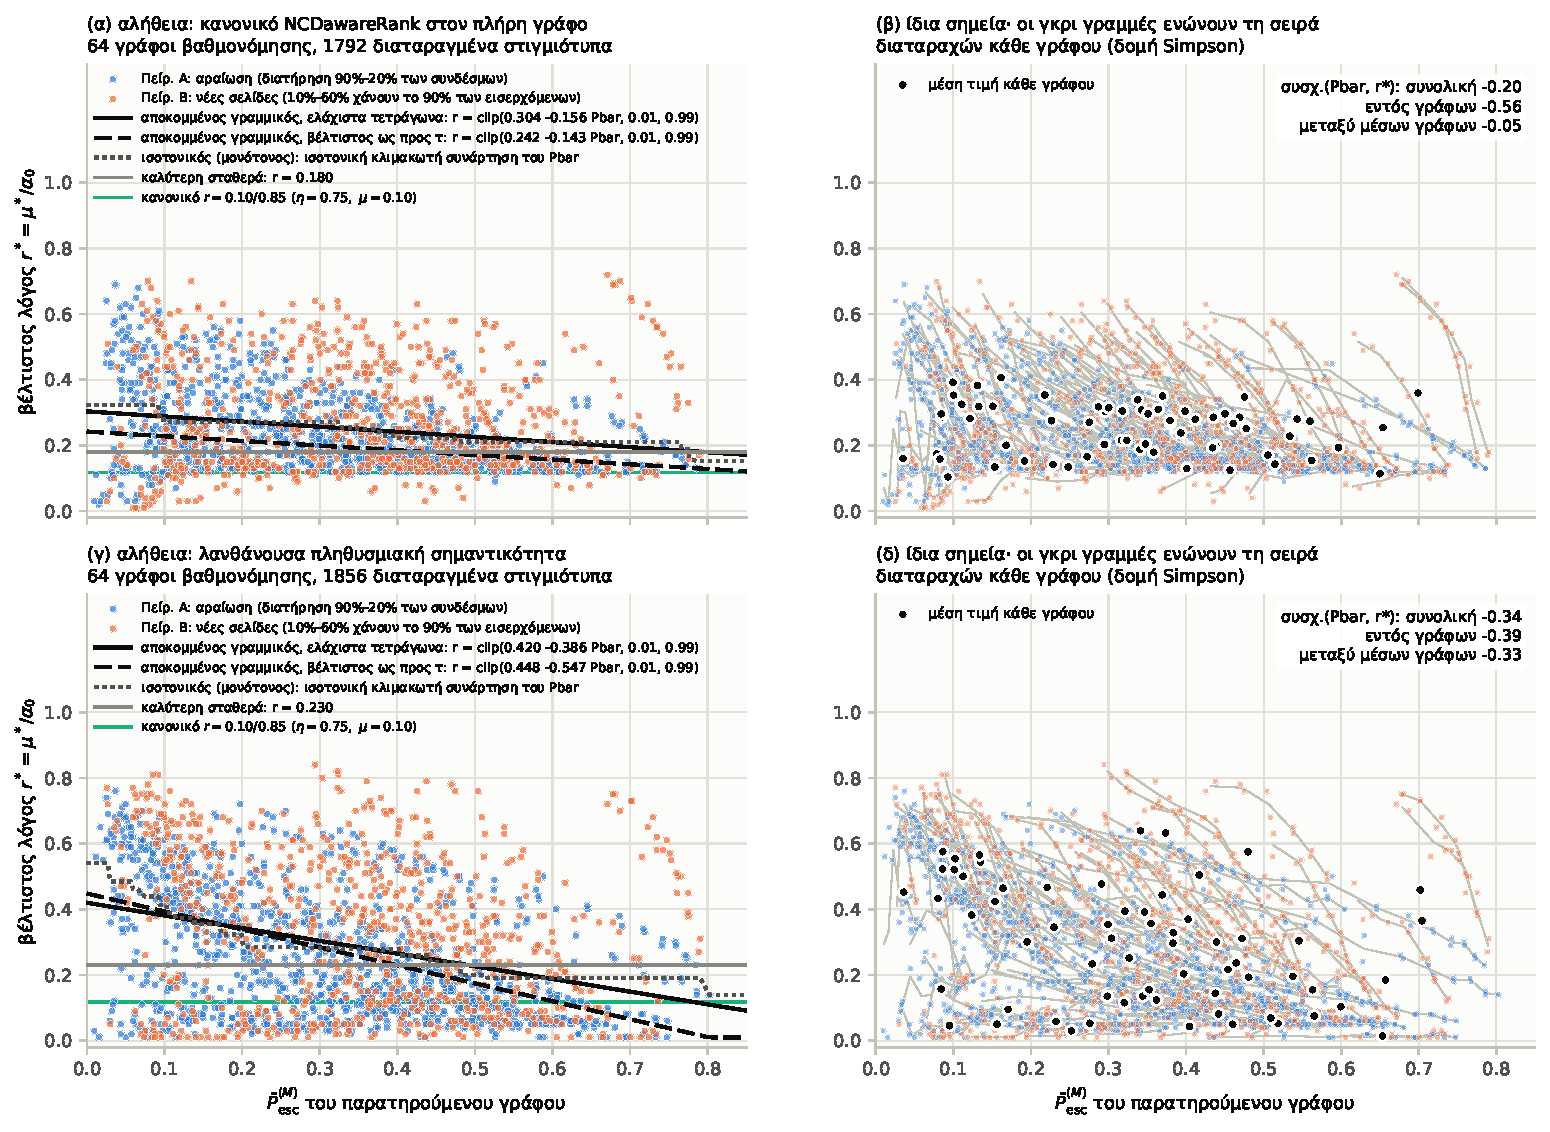
\includegraphics[width=\textwidth]{stage1_calibration_scatter.pdf}
\caption{Στάδιο~1: βέλτιστος λόγος $r^*$ έναντι του $\Pbar$ του παρατηρούμενου γράφου στο σύνολο
βαθμονόμησης. \textbf{(α)} Αλήθεια NCD με τους προσαρμοσμένους υποψήφιους κανόνες και το κανονικό $r$.
\textbf{(γ)} Αλήθεια POP. \textbf{(β,\,δ)} Τα ίδια σημεία, με γκρι γραμμές που ενώνουν τη σειρά
διαταραχών κάθε γράφου και μαύρες κουκκίδες που σημειώνουν τις μέσες τιμές των γράφων. Η συνολική κλίση
είναι μείγμα μιας απότομης σχέσης εντός γράφων και μιας σχεδόν επίπεδης σχέσης μεταξύ γράφων.}
\label{fig:s1scatter}
\end{figure}

\subsection{Γιατί το \texorpdfstring{$\Pbar$}{P̄} δεν μεταφέρεται: δομή Simpson}
Η συνολική συσχέτιση μεταξύ $\Pbar$ και $r^*$ είναι \SOnePooled. Εντός γράφων είναι \SOneWithin{}
(\SOneWithinA{} στο Πείραμα~Α και \SOneWithinB{} στο Πείραμα~Β), και μεταξύ των μέσων τιμών των γράφων
είναι \SOneBetween. Εντός ενός γράφου, το $\Pbar$ απλώς ακολουθεί το πόσους συνδέσμους αφαίρεσε η
διαταραχή: η συσχέτισή του εντός γράφων με το ποσοστό των τόξων που διατηρήθηκαν είναι \SOnePkeepA{}
(Α) και \SOnePkeepB{} (Β). Η αφαίρεση συνδέσμων μειώνει τόσο το $\Pbar$ όσο και τη συμφωνία μεταξύ
παρατηρούμενου και πλήρους γράφου, και η δεύτερη απαιτεί μεγαλύτερο βάρος στην εξομάλυνση σε επίπεδο
μπλοκ που επιτελεί ο $M$. Μεταξύ γράφων, όμως, το επίπεδο του $\Pbar$ δεν λέει σχεδόν τίποτα για το
$r^*$. Ένας χρήστης παρατηρεί έναν μόνο γράφο και δεν μπορεί να διακρίνει αν ένα χαμηλό $\Pbar$
οφείλεται σε έντονη απώλεια συνδέσμων ή σε έναν γράφο που είναι εκ φύσεως περιορισμένος εντός των
μπλοκ. Η προσαρμοσμένη κλίση είναι επομένως ελάχιστα χρήσιμη εκτός δείγματος.

\subsection{Τι καθορίζει το \texorpdfstring{$r^*$}{r*}}
Ο Πίνακας~\ref{tab:stage1dec} αποσυνθέτει τη διασπορά του $r^*$ υπό κάθε αλήθεια. Υπό την NCD, η
ταυτότητα του γράφου εξηγεί \SOneDecBase{} και το επίπεδο διαταραχής \SOneDecLevel{}· προσθετικά
εξηγούν \SOneDecBL. Ενισχυμένα δέντρα στις \emph{κρυφές} παραμέτρους της γεννήτριας μαζί με το επίπεδο
ανακτούν \SOneDecHidden{} εκτός δείγματος, ενώ όλα τα παρατηρήσιμα στατιστικά μαζί ανακτούν
$\SOneDecObs$ και το $\Pbar$ μόνο του $\SOneDecP$. Η συνιστώσα σε επίπεδο γράφου συνδέεται με τη
λανθάνουσα δομή ποιότητας. Η μέση τιμή του $r^*$ ανά γράφο συσχετίζεται κατά \SOneCorrICC{} με τον ICC
και κατά \SOneCorrFit{} με τη διασπορά της λανθάνουσας ποιότητας υπό την NCD, και κατά
\SOneCorrICCPop{} και \SOneCorrFitPop{} υπό την POP (Σχήμα~\ref{fig:s1diag}(γ)). Αυτό είναι το
καθεστώς στο οποίο αποδίδει η συρρίκνωση προς τους μέσους όρους των μπλοκ, δηλαδή αυτό που επιτελεί ο
$M$. Κανένα από τα δύο μεγέθη δεν είναι ορατό σε καθολικά στατιστικά του παρατηρούμενου γράφου. Η
συσχέτιση ελέγχου--επανελέγχου του $r^*$ μεταξύ των επαναλήψεων είναι \SOneRetest, οπότε το ανεξήγητο
μέρος δεν είναι θόρυβος του μαντείου.

\begin{table}[t]
\centering
\footnotesize
\caption{Ποσοστό της διασποράς του βέλτιστου λόγου $r^*$ που εξηγείται ($R^2$) στο σύνολο βαθμονόμησης. Η ταυτότητα του γράφου, το επίπεδο διαταραχής και ο προσθετικός τους συνδυασμός είναι μερίδια ANOVA εντός δείγματος. Οι στήλες με αστερίσκο είναι εκτός δείγματος (ομαδοποιημένη 8-πλή CV ανά γράφο): ενισχυμένα δέντρα στις κρυφές παραμέτρους της γεννήτριας μαζί με το επίπεδο διαταραχής· παλινδρόμηση ridge σε όλα τα παρατηρήσιμα καθολικά στατιστικά· και ο αποκομμένος γραμμικός κανόνας στο $\bar P^{(M)}_{\mathrm{esc}}$. Αρνητικές τιμές σημαίνουν χειρότερη πρόβλεψη από τη μέση τιμή.}
\label{tab:stage1dec}
\begin{tabular}{@{}lrrrrrr@{}}
\toprule
αλήθεια & γράφος & επίπεδο & γράφος+επίπεδο & κρυφές+επίπεδο$^{*}$ & όλα τα παρατηρ.$^{*}$ & μόνο $\bar P^{(M)}_{\mathrm{esc}}$$^{*}$ \\
\midrule
NCD & 0.31 & 0.42 & 0.74 & 0.71 & -0.01 & 0.03 \\
PR & 0.41 & 0.30 & 0.71 & 0.70 & -0.08 & -0.02 \\
POP & 0.74 & 0.13 & 0.87 & 0.63 & 0.11 & 0.07 \\
SELF & 0.34 & 0.04 & 0.38 & -0.36 & -0.02 & 0.00 \\
\bottomrule
\end{tabular}
\end{table}


\subsection{Ευαισθησία ως προς την αλήθεια αναφοράς}
\label{sec:res1-truth}
Το Σχήμα~\ref{fig:s1truth} επαναλαμβάνει την ανάλυση υπό και τις τέσσερις αλήθειες. Υπό την PR, το
\SOnePrLower\% των βέλτιστων λόγων βρίσκεται στο κάτω όριο $r=0.01$, επειδή μια αναφορά PageRank
ευνοεί $r\to0$. Υπό την POP, η σχέση με το $\Pbar$ είναι αρνητική τόσο εντός γράφων (\SOnePopWithinT)
όσο και μεταξύ γράφων (\SOnePopBetweenT), αλλά ο προσαρμοσμένος κανόνας και πάλι δεν υπερέχει μιας
σταθεράς εκτός δείγματος (Πίνακας~\ref{tab:stage1truth} του Παραρτήματος). Υπό την SELF, το πρωτόκολλο
του~\cite{ng13}, το \SOneSelfUpper\% των βέλτιστων λόγων βρίσκεται στο άνω όριο $r=0.99$. Η σύγκριση
μιας κατάταξης με τη \emph{δική της} κατάταξη στον πλήρη γράφο επιβραβεύει οτιδήποτε καθιστά την
κατάταξη αναίσθητη στους συνδέσμους: ένα μεγάλο $r$ εξομαλύνει τη βαθμολογία πάνω στα μπλοκ, τα οποία
δεν διαταράσσονται. Το ίδιο ισχύει για το $\alpha$: καθώς $\alpha\to0$, και οι δύο κατατάξεις τείνουν
στο $v$, το οποίο εξαρτάται μόνο από τη διαμέριση, οπότε $\tau\to1$. Η σταθερότητα είναι θεμιτή
ιδιότητα προς αναφορά, αλλά δεν μπορεί να χρησιμεύσει ως στόχος για την επιλογή παραμέτρων.

\begin{figure}[t]
\centering
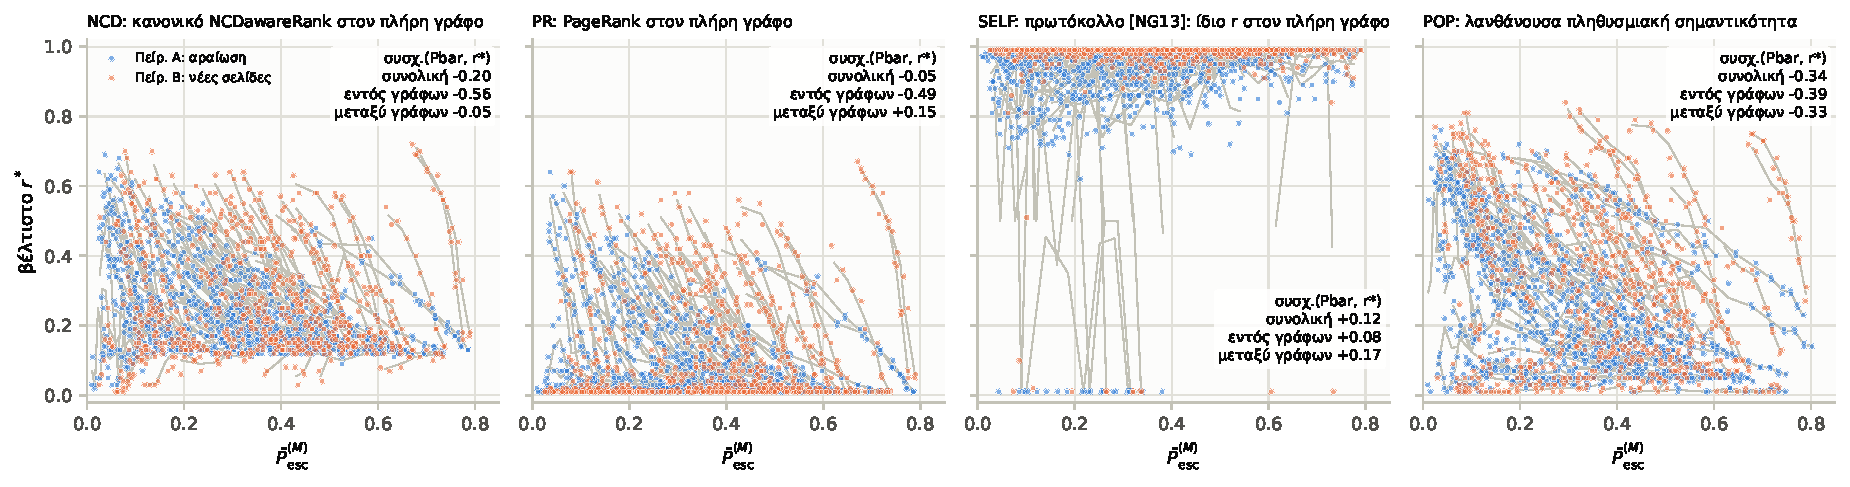
\includegraphics[width=\textwidth]{stage1_gt_sensitivity.pdf}
\caption{Βέλτιστος λόγος του Σταδίου~1 έναντι του $\Pbar$ υπό τις τέσσερις αλήθειες του Σταδίου~1
(σύνολο βαθμονόμησης). Υπό την SELF, το πρωτόκολλο του~\cite{ng13}, το μαντείο ωθείται στο άνω όριο του
πλέγματος.}
\label{fig:s1truth}
\end{figure}

\begin{figure}[t]
\centering
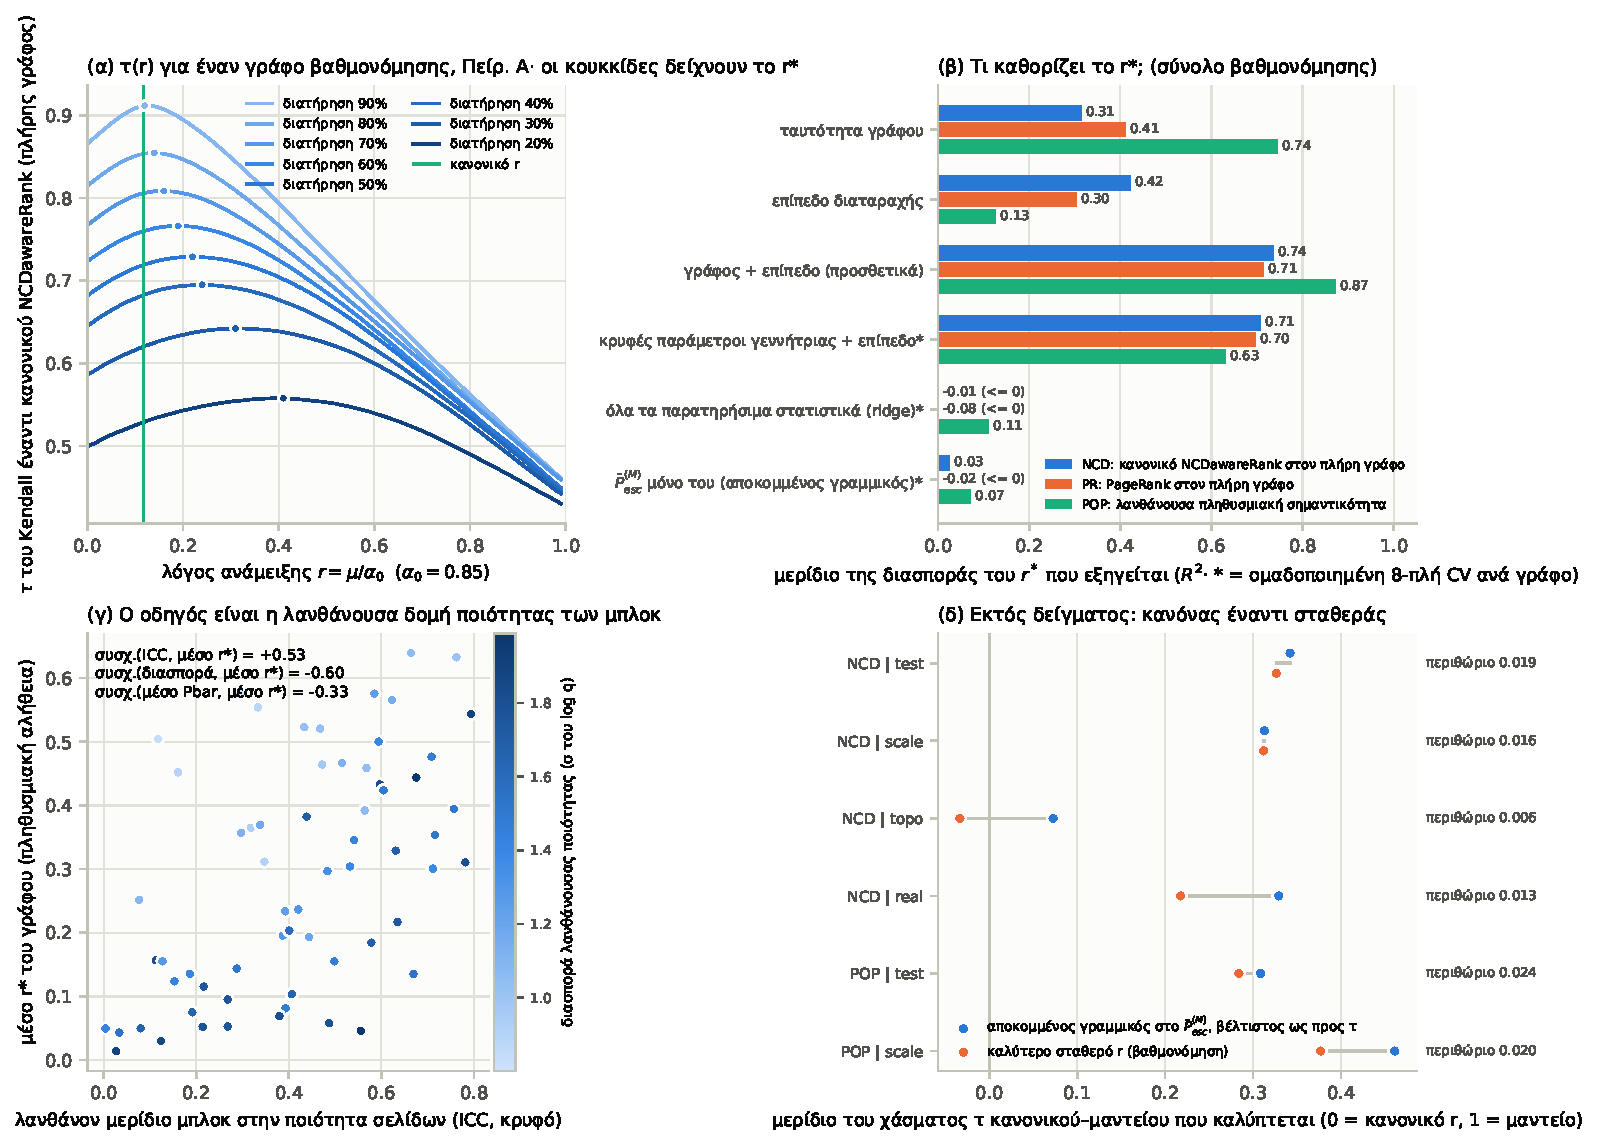
\includegraphics[width=\textwidth]{stage1_diagnostics.pdf}
\caption{Διαγνωστικά του Σταδίου~1. \textbf{(α)} Καμπύλες $\tau(r)$ για έναν γράφο βαθμονόμησης υπό
αυξανόμενη απώλεια συνδέσμων· οι κουκκίδες σημειώνουν το $r^*$, το οποίο απομακρύνεται από την κανονική
τιμή καθώς χάνονται σύνδεσμοι. \textbf{(β)} Μερίδιο της διασποράς του $r^*$ που εξηγεί κάθε πηγή.
\textbf{(γ)} Μέσο $r^*$ ανά γράφο υπό την POP έναντι του λανθάνοντος ICC, χρωματισμένο κατά τη διασπορά
της λανθάνουσας ποιότητας. \textbf{(δ)} Μερίδιο του χάσματος κανονικού--μαντείου που καλύπτεται εκτός
δείγματος από τον κανόνα και από την καλύτερη σταθερά.}
\label{fig:s1diag}
\end{figure}

\subsection{Πραγματικά δίκτυα}
Ανά γράφο, ο κανόνας του Σταδίου~1 μεταβάλλει το $\tau$ σε σχέση με την κανονική ρύθμιση κατά
\SOneRealCiteseer{} (CiteSeer), \SOneRealCnr{} (cnr-2000), \SOneRealCorafull{} (Cora), \SOneRealCoraml{}
(Cora-ML) και \SOneRealWikics{} (WikiCS). Το κέρδος σε επίπεδο συνόλου προέρχεται μόνο από το CiteSeer,
έναν πολύ αραιό γράφο (μέσος βαθμός εξόδου $1.27$) του οποίου το $95\%$ των τόξων βρίσκεται εντός μπλοκ.
Επιπλέον, εκεί ο προσαρμοσμένος κανόνας εφαρμόζεται με παρέκταση: το $\Pbar=\PbarCiteseer$ του CiteSeer
βρίσκεται στο άκρο του εύρους βαθμονόμησης. Στο cnr-2000 ($\Pbar=\PbarCnr$) ο κανόνας ορίζει
$r=\RuleRCnr$, δηλαδή $\mu=\RuleMuCnr$ για $\alpha=0.85$, περίπου το διπλάσιο του κανονικού $\mu$, και
υστερεί σε $\tau$ έναντι αυτού. Ο κανόνας επιστρέφει $r\approx0.12$ μόνο για $\Pbar\approx0.85$, τιμή
που κανένας πραγματικός γράφος της μελέτης δεν προσεγγίζει.

\FloatBarrier
% =============================================================================
\section{Αποτελέσματα: Στάδιο~2, η συνολική απόσβεση}
\label{sec:res2}

\subsection{Υποψήφιοι κανόνες}
Το Σχήμα~\ref{fig:s2scatter}(α) απεικονίζει τη βέλτιστη απόσβεση $\alpha^*$ έναντι του $h$ για τους
γράφους βαθμονόμησης, με το $r$ κλειδωμένο στον κανόνα του Σταδίου~1· ο Πίνακας~\ref{tab:stage2}
παρουσιάζει κάθε υποψήφιο κανόνα. Το μαντείο είναι $\alpha^*=\STwoAstarMean\pm\STwoAstarSd$. Ο
αποκομμένος γραμμικός κανόνας που είναι βέλτιστος ως προς $\tau$ συγκλίνει στη σταθερά
$\alpha=\clip(0.810-0.000\,h)=\STwoConstAlpha$: όταν στόχος είναι η συμφωνία κατατάξεων, η κλίση ως προς
$h$ μηδενίζεται. Κάθε υποψήφιος κανόνας που πράγματι εξαρτάται από το $h$ είναι χειρότερος από τη
σταθερά.
\begin{itemize}[leftmargin=1.4em,itemsep=0pt]
\item Ο κανόνας ελαχίστων τετραγώνων $\clip(\STwoLSa\STwoLSb\,h)$ χάνει \STwoTestLSvsConst{} στο
\texttt{test} ($p=\STwoTestLSvsConstP$) και \STwoTopoLSvsConst{} στο \texttt{topo}
($p=\STwoTopoLSvsConstP$).
\item Ο ισοτονικός κανόνας χάνει \STwoTestIsoVsConst{} ($p=\STwoTestIsoVsConstP$) στο \texttt{test}.
\item Ο κανόνας προϋπολογισμού μετατόπισης $c/(c+h)$, $c=\STwoBudgetC$, χάνει \STwoTestBudVsConst{} στο
\texttt{test} και \STwoScaleBudVsConst{} στο \texttt{scale}.
\item Τα ενισχυμένα δέντρα σε όλα τα παρατηρήσιμα στατιστικά, μαζί με τα $h$ και $h_v$, είναι ο πιο
ευέλικτος υποψήφιος, όμως χάνουν \STwoTopoGbmVsConst{} στο \texttt{topo} ($p=\STwoTopoGbmVsConstP$).
\item Η αντικατάσταση του $h$ από το $h_v$ δεν αλλάζει τίποτα (ο κανόνας ελαχίστων τετραγώνων
$\clip(\STwoLSva\STwoLSvb\,h_v)$ χάνει \STwoTestLSvVsConst{} στο \texttt{test},
$p=\STwoTestLSvVsConstP$).
\end{itemize}
Η ίδια η σταθερά βελτιώνει το $\alpha=0.85$ κατά \STwoTestConstVs{} στο \texttt{test}
($p=\STwoTestConstP$), \STwoScaleConstVs{} στο \texttt{scale} και \STwoTopoConstVs{} στο \texttt{topo},
καλύπτοντας το \STwoTestConstGap\%, το \STwoScaleConstGap\% και το \STwoTopoConstGap\% του χάσματος προς
το μαντείο. Στο \texttt{real} μεταβάλλει το $\tau$ κατά \STwoRealConstVs{} ($p=\STwoRealConstP$).

\begin{table*}[t]
\centering
\footnotesize
\caption{Υποψήφιοι κανόνες του Σταδίου~2, $\alpha=g(h)$ και $\alpha=g(h_v)$, με το $r$ κλειδωμένο στον κανόνα του Σταδίου~1 και αλήθεια NCD. Άνω τμήμα: μέσο $\tau$ του Kendall για τη στατική απόσβεση, την κλειδωμένη σταθερά, τη διαφορά τους και το μαντείο. Κάτω τμήματα: διαφορά του μέσου $\tau$ κάθε προσαρμοσμένου κανόνα έναντι της κλειδωμένης σταθεράς. CV $\tau$: ομαδοποιημένη 8-πλή διασταυρωμένη επικύρωση στους γράφους βαθμονόμησης. $^{\dagger}$: $p<0.01$ στον έλεγχο προσημασμένων τάξεων του Wilcoxon ανά γράφο. Όλοι οι κανόνες αποκόπτονται στο $[0.40,0.99]$· ΕΤ: ελάχιστα τετράγωνα στις βέλτιστες τιμές· βέλτ.\ $\tau$: προσαρμογή με μεγιστοποίηση του μέσου $\tau$ βαθμονόμησης.}
\label{tab:stage2}
\begin{tabular}{@{}llrrrrr@{}}
\toprule
κανόνας & τύπος & CV $\tau$ & \texttt{test} & \texttt{scale} & \texttt{topo} & \texttt{real} \\
\midrule
\multicolumn{7}{@{}l}{\emph{μέσο $\tau$ του Kendall}} \\
στατικό $\alpha=0.85$ & & -- & 0.6867 & 0.6681 & 0.7844 & 0.7600 \\
σταθερό $\alpha=0.810$ (κλειδωμένο) & & 0.6913 & 0.6911 & 0.6735 & 0.7875 & 0.7559 \\
\quad διαφορά & &  & $+$0.0044$^{\dagger}$ & $+$0.0054$^{\dagger}$ & $+$0.0031$^{\dagger}$ & $-$0.0012 \\
μαντείο $\alpha^*$ & & -- & 0.6960 & 0.6787 & 0.7911 & 0.7738 \\
\midrule
\multicolumn{7}{@{}l}{\emph{κανόνες στο $h$: διαφορά μέσου $\tau$ έναντι της κλειδωμένης σταθεράς}} \\
αποκομμένος γραμμικός, βέλτ.\ $\tau$ (κλειδ.) & $\mathrm{clip}(0.810-0.000\,h)$ & 0.6912 & 0.0000 & 0.0000 & 0.0000 & 0.0000 \\
αποκομμένος γραμμικός, ΕΤ & $\mathrm{clip}(0.803-0.021\,h)$ & 0.6898 & $-$0.0015$^{\dagger}$ & $-$0.0013 & $-$0.0007$^{\dagger}$ & $-$0.0033 \\
ισοτονικός & -- & 0.6897 & $-$0.0016$^{\dagger}$ & $-$0.0014 & $-$0.0010$^{\dagger}$ & $-$0.0049 \\
προϋπολ.\ $c/(c+x)$, βέλτ.\ $\tau$ & $c=2.69$ & 0.6891 & $-$0.0023$^{\dagger}$ & $-$0.0043$^{\dagger}$ & $-$0.0016$^{\dagger}$ & $-$0.0045 \\
ενισχυμένα δέντρα, όλα τα παρατηρ. & -- & 0.6905 & $-$0.0002 & $-$0.0030 & $-$0.0018$^{\dagger}$ & $-$0.0124 \\
\midrule
\multicolumn{7}{@{}l}{\emph{κανόνες στο $h_v$: διαφορά μέσου $\tau$ έναντι της κλειδωμένης σταθεράς}} \\
αποκομμένος γραμμικός, βέλτ.\ $\tau$ (κλειδ.) & $\mathrm{clip}(0.810+0.000\,h_v)$ & 0.6912 & 0.0000 & 0.0000 & 0.0000 & 0.0000 \\
αποκομμένος γραμμικός, ΕΤ & $\mathrm{clip}(0.802-0.016\,h_v)$ & 0.6898 & $-$0.0015$^{\dagger}$ & $-$0.0013 & $-$0.0011$^{\dagger}$ & $-$0.0029 \\
ισοτονικός & -- & 0.6896 & $-$0.0018$^{\dagger}$ & $-$0.0013 & $-$0.0024$^{\dagger}$ & $-$0.0037 \\
προϋπολ.\ $c/(c+x)$, βέλτ.\ $\tau$ & $c=3.04$ & 0.6888 & $-$0.0024 & $-$0.0037 & $-$0.0083$^{\dagger}$ & $-$0.0019 \\
\bottomrule
\end{tabular}
\end{table*}


\begin{figure}[p]
\centering
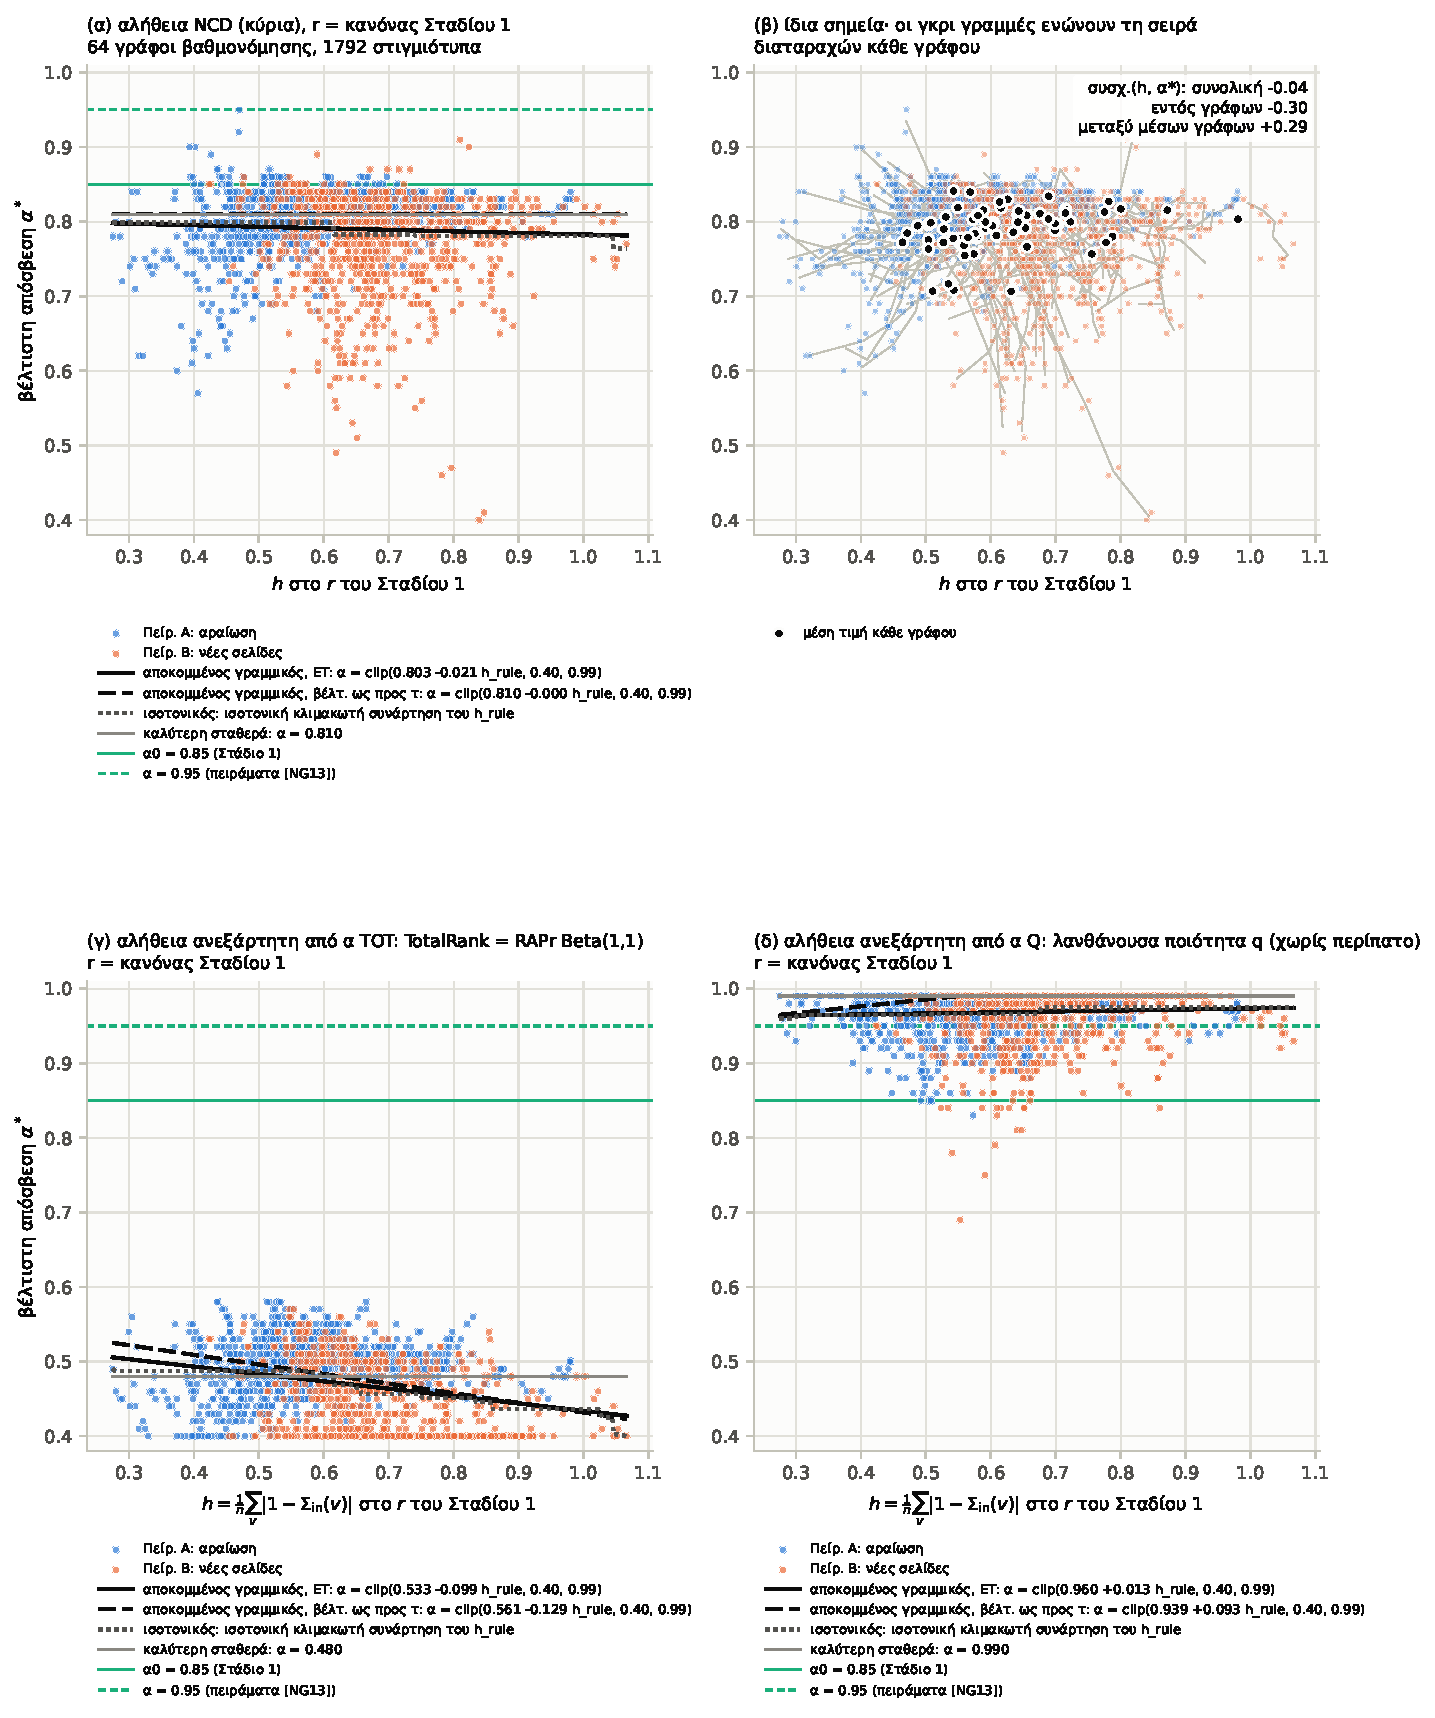
\includegraphics[width=0.94\textwidth]{stage2_calibration_scatter.pdf}
\caption{Στάδιο~2: βέλτιστη απόσβεση $\alpha^*$ έναντι του $h$ (υπολογισμένου στο $r$ του Σταδίου~1)
στο σύνολο βαθμονόμησης. \textbf{(α)} Κύρια αλήθεια NCD με τους προσαρμοσμένους υποψήφιους κανόνες της
$g$. Οι προσαρμογές ελαχίστων τετραγώνων και βέλτιστης ως προς $\tau$ είναι σχεδόν επίπεδες, και η
δεύτερη συμπίπτει με τη σταθερά $0.810$. \textbf{(β)} Τα ίδια σημεία, με ενωμένη τη σειρά διαταραχών
κάθε γράφου. \textbf{(γ,\,δ)} Οι δύο αλήθειες που δεν εξαρτώνται από το $\alpha$, η TOT
($\alpha^*\approx0.47$) και η Q ($\alpha^*$ κοντά στην κορυφή του πλέγματος). Οριζόντιες γραμμές:
$\alpha_0=0.85$ και το $\alpha=0.95$ του~\cite{ng13}.}
\label{fig:s2scatter}
\end{figure}

\subsection{Γιατί το \texorpdfstring{$h$}{h} δεν μπορεί να παρακολουθήσει το \texorpdfstring{$\alpha^*$}{α*}}
\label{sec:hmech}
Η συνολική συσχέτιση μεταξύ $h$ και $\alpha^*$ είναι \STwoPooled. Εντός γράφων είναι \STwoWithin, και
μεταξύ των μέσων τιμών των γράφων \STwoBetween{} (για το $h_v$: \STwoWithinHv{} και \STwoBetweenHv). Η
τιμή εντός γράφων είναι η ίδια μείγμα δύο αντίθετων μηχανισμών, ενός για κάθε διαταραχή:
\begin{itemize}[leftmargin=1.4em,itemsep=1pt]
\item \emph{Το Πείραμα~Α (ομοιόμορφη αφαίρεση συνδέσμων) μειώνει το $h$.} Το μέσο $h$ πέφτει από
\STwoHmildA{} όταν διατηρείται το $90\%$ των τόξων σε \STwoHsevereA{} όταν διατηρείται το $20\%$
(συσχέτιση εντός γράφων με το ποσοστό διατήρησης \STwoHkeepA). Η αφαίρεση τόξων δημιουργεί κρεμάμενες
σελίδες, και οι ομοιόμορφες γραμμές τους προσθέτουν $n_{\mathrm d}/n$ σε κάθε άθροισμα στήλης, έλκοντας
το $\Sin$ προς το~$1$ (συσχέτιση του $h$ με το ποσοστό κρεμάμενων σελίδων \STwoHdangA).
\item \emph{Το Πείραμα~Β (νεοεισαχθείσες σελίδες) αυξάνει το $h$}, από \STwoHmildB{} σε \STwoHsevereB{}:
οι σελίδες που χάνουν το $90\%$ των εισερχόμενων συνδέσμων τους αποκτούν $\Sin\approx0$ (συσχέτιση του
$h$ με το μερίδιο σελίδων μηδενικής εισροής \STwoHzinB).
\end{itemize}
Και στα δύο πειράματα το $\alpha^*$ \emph{μειώνεται} με τη σφοδρότητα της διαταραχής, από \STwoAmildA{}
σε \STwoAsevereA{} (Α) και από \STwoAmildB{} σε \STwoAsevereB{} (Β). Η συσχέτιση εντός γράφων του $h$ με
το $\alpha^*$ είναι επομένως \STwoHastarA{} υπό το Α και \STwoHastarB{} υπό το Β. Ένα στατιστικό που
αυξάνεται υπό το ένα είδος απώλειας συνδέσμων και μειώνεται υπό το άλλο, ενώ η βέλτιστη απόσβεση
μειώνεται και στα δύο, δεν μπορεί να βαθμονομήσει το $\alpha$. Η αρχική υπόθεση ότι μεγαλύτερο $h$
απαιτεί μεγαλύτερο $\alpha$ διαψεύδεται, όπως και η αντίθετή της. Ο Πίνακας~\ref{tab:stage2dec} το
ποσοτικοποιεί. Υπό την NCD, το $h$ μόνο του εξηγεί $\STwoDecH$ της διασποράς του $\alpha^*$ εκτός
δείγματος, και το πολύ \STwoDecHmax{} υπό οποιαδήποτε αλήθεια. Η ταυτότητα του γράφου εξηγεί
\STwoDecBase{} και το επίπεδο διαταραχής, που δεν είναι παρατηρήσιμο στην πράξη, \STwoDecLevel·
ενισχυμένα δέντρα στις κρυφές παραμέτρους της γεννήτριας μαζί με το επίπεδο ανακτούν \STwoDecHidden{}
εκτός δείγματος, ενώ όλα τα παρατηρήσιμα στατιστικά μαζί ανακτούν μόνο \STwoDecObs.

\begin{table}[t]
\centering
\footnotesize
\caption{Ποσοστό της διασποράς της βέλτιστης απόσβεσης $\alpha^*$ που εξηγείται ($R^2$) στο σύνολο βαθμονόμησης, για κάθε αλήθεια και ρύθμιση του $r$. Η ταυτότητα του γράφου, το επίπεδο διαταραχής και ο προσθετικός τους συνδυασμός είναι μερίδια ANOVA εντός δείγματος. Οι στήλες με αστερίσκο είναι εκτός δείγματος (ομαδοποιημένη 8-πλή CV ανά γράφο): ενισχυμένα δέντρα στις κρυφές παραμέτρους της γεννήτριας μαζί με το επίπεδο διαταραχής· παλινδρόμηση ridge σε όλα τα παρατηρήσιμα καθολικά στατιστικά, μαζί με τα $h$ και $h_v$· και ο αποκομμένος γραμμικός κανόνας μόνο στο $h$. Αρνητικές τιμές σημαίνουν χειρότερη πρόβλεψη από τη μέση τιμή.}
\label{tab:stage2dec}
\begin{tabular}{@{}llrrrrrr@{}}
\toprule
αλήθεια & $r$ & γράφος & επίπεδο & γράφος+επίπεδο & κρυφές+επίπεδο$^{*}$ & όλα τα παρατηρ.$^{*}$ & μόνο $h$$^{*}$ \\
\midrule
NCD & Στάδιο~1 & 0.25 & 0.47 & 0.72 & 0.60 & 0.17 & $-$0.02 \\
NCD & 0.118 & 0.32 & 0.41 & 0.73 & 0.62 & 0.13 & $-$0.03 \\
NCD95 & 0.105 & 0.40 & 0.22 & 0.62 & 0.38 & 0.10 & $-$0.03 \\
TOT & Στάδιο~1 & 0.10 & 0.77 & 0.87 & 0.87 & 0.18 & 0.05 \\
POP & κανόνας POP & 0.54 & 0.29 & 0.83 & 0.44 & 0.28 & $-$0.03 \\
Q & Στάδιο~1 & 0.67 & 0.02 & 0.69 & $-$0.20 & 0.05 & $-$0.03 \\
\bottomrule
\end{tabular}
\end{table}


\begin{table}[t]
\centering
\small
\caption{Τα Πειράματα Α και Β είναι μείγματα επιδράσεων κρεμάμενων σελίδων και μηδενικών εισερχόμενων συνδέσεων. Οι τιμές εκτείνονται από την ηπιότερη έως τη σοβαρότερη στάθμη.}
\label{tab:mixture}
\begin{tabular}{@{}lrrrr@{}}\toprule
πείραμα & $\delta$ & $\zeta$ & $h$ & $h_{\rm raw}$ \\
\midrule
Α: διατήρηση τόξων 1.0$\to$0.2 & 0.173$\to$0.483 & 0.156$\to$0.506 & 0.620$\to$0.476 & 0.679$\to$0.669 \\
Β: απώλεια σελίδων 0.1$\to$0.6 & 0.185$\to$0.298 & 0.207$\to$0.461 & 0.644$\to$0.704 & 0.707$\to$0.827 \\
\bottomrule\end{tabular}
\end{table}


Τα Πειράματα Α και Β είναι μείγματα δημιουργίας κρεμάμενων σελίδων, σελίδων χωρίς εισερχόμενες
συνδέσεις και μεταβολής της μάζας μετάβασης, με διαφορετικές αναλογίες. Ο παραγόμενος πίνακας
το κάνει ρητό. Ειδικά, το $h_{\rm raw}$ μόνο του είναι σχεδόν τυφλό στο Α και επομένως δεν αποτελεί
γενικό μέτρο σοβαρότητας και για τα δύο πρωτόκολλα διαταραχής.

\paragraph{Μη μονότονοι κανόνες και κανόνες χωρίς την επίδραση των κρεμάμενων σελίδων.}
Επειδή το $\alpha^*$ μειώνεται και υπό τις δύο διαταραχές, ενώ το $h$ κινείται σε αντίθετες
κατευθύνσεις, εντός ενός γράφου το $\alpha^*$ σχηματίζει ανεστραμμένο V ως προς το $h$ γύρω από την τιμή
$h_0$ του αδιατάρακτου γράφου (οι ενωμένες σειρές του Σχήματος~\ref{fig:s2scatter}(β)). Η απόσταση από
αυτή την κορυφή φέρει πραγματική πληροφορία: το $|h-h_0|$ συσχετίζεται κατά \NmDistOwn{} με το
$\alpha^*$ (\NmDistOwnWithin{} εντός γράφων). Αναζητήσαμε επομένως κανόνα που να εκμεταλλεύεται το σχήμα
(σενάριο \texttt{stage2\_nonmonotone\_search.py}· Πίνακας~\ref{tab:nonmono}). Ασύμμετρες τέντες
$\clip\bigl(\alpha_{\mathrm{peak}}-s_L\max(0,h_0-h)-s_R\max(0,h-h_0),\,0.40,\,0.99\bigr)$, συμμετρικές
τέντες, μια κοίλη τετραγωνική συνάρτηση, ένα γκαουσιανό εξόγκωμα, κλιμακωτές συναρτήσεις δύο και τριών
περιοχών και μια γραμμική spline δύο κόμβων προσαρμόστηκαν στα $h$ και $h_v$, τόσο με ελάχιστα
τετράγωνα στο $\alpha^*$ όσο και με απευθείας μεγιστοποίηση του μέσου $\tau$ (ακριβώς για τις
κλιμακωτές συναρτήσεις· για τις υπόλοιπες με αναζήτηση πλέγματος, με την κορυφή των κανόνων στο $h$ στο
$[0.50,0.70]$, και στη συνέχεια Nelder--Mead και Powell). Αξιολογήθηκαν ακριβώς όπως οι
υπόλοιποι υποψήφιοι: 8-πλή διασταυρωμένη επικύρωση ανά γράφο στο \texttt{calib}, με τη σταθερά
επαναπροσαρμοσμένη σε κάθε τμήμα, και στη συνέχεια τα τέσσερα σύνολα εκτός δείγματος. Η βέλτιστη ως προς
$\tau$ τέντα τοποθετεί την κορυφή της στο $h_0=\NmTentHzero$, με $\alpha_{\mathrm{peak}}=\NmTentPeak$,
$s_L=\NmTentSL$ και $s_R=\NmTentSR$. Ακολουθεί μέρος της μεταβολής εντός γράφων (οι προβλέψεις της
συσχετίζονται κατά \NmTentWithin{} με το $\alpha^*$ εντός γράφων), όμως μεταβάλλει το μέσο $\tau$ μόνο
κατά \NmTentCalib{} εντός δείγματος, \NmTentCV{} στη διασταυρωμένη επικύρωση ($p=\NmTentCVP$) και
\NmTentHeld{} στους 73 γράφους εκτός δείγματος ($p=\NmTentHeldP$). Κανένας μη μονότονος κανόνας βέλτιστος ως προς $\tau$ στο $h$
ή στο $h_v$ δεν κερδίζει περισσότερο από \NmMaxOneDCV{} στη διασταυρωμένη επικύρωση ή \NmMaxOneDHeld{}
εκτός δείγματος, και οι προσαρμογές ελαχίστων τετραγώνων μεταβάλλουν το $\tau$ κατά \NmLSBest{} έως
\NmLSWorst{} εκτός δείγματος.

Η αφαίρεση της ομοιόμορφης συνεισφοράς $(1-r)\,\delta$ των κρεμάμενων σελίδων, με
$\delta=n_{\mathrm d}/n$, από κάθε άθροισμα στήλης ελέγχει αν η πτώση του $h$ υπό το Πείραμα~Α είναι τεχνούργημα των
κρεμάμενων σελίδων. Σε μεγάλο βαθμό είναι: η απόκλιση χωρίς την επίδραση των κρεμάμενων σελίδων
$h_{\mathrm{raw}}=\frac1n\sum_v|1-\Sin(v)+(1-r)\delta|$ σχεδόν δεν μεταβάλλεται υπό το Α (\NmHrawFull{}
στον αδιατάρακτο γράφο, \NmHrawSevA{} όταν διατηρείται το $20\%$ των τόξων) και αυξάνεται υπό το Β
(\NmHrawSevB{} στο $60\%$). Δύο ακόμη παραλλαγές αυξάνονται και υπό τις δύο διαταραχές: η σχετική
διασπορά $h_{\mathrm{raw}}^{\mathrm{rel}}$ των διορθωμένων αθροισμάτων (από \NmHrelFull{} σε
\NmHrelSevA{} υπό το Α και \NmHrelSevB{} υπό το Β) και η απόκλιση $h_{\mathrm{raw}}^{H}$ των αθροισμάτων
στηλών του πίνακα υπερσυνδέσμων πριν από τη διόρθωση των κρεμάμενων γραμμών του (από \NmHHFull{} σε
\NmHHSevA{} και \NmHHSevB). Εντός γράφων, και οι δύο συσχετίζονται αρνητικά με το $\alpha^*$ υπό κάθε
πείραμα (\NmHrelAstarA{} και \NmHrelAstarB{} για το $h_{\mathrm{raw}}^{\mathrm{rel}}$). Η απαλοιφή της
επίδρασης των κρεμάμενων σελίδων μετατρέπει λοιπόν το ανεστραμμένο V σε μονότονη σχέση, αλλά μόνο εντός
κάθε γράφου. Η αδιατάρακτη τιμή του $h_{\mathrm{raw}}^{\mathrm{rel}}$ μεταβάλλεται μεταξύ γράφων με
τυπική απόκλιση \NmRelSd, έναντι μετατοπίσεων εντός γράφου \NmRelExcA{} (Α) και \NmRelExcB{} (Β), και
συσχετίζεται \emph{θετικά} με τη μέση τιμή του $\alpha^*$ ανά γράφο (\NmRelBetween): πρόκειται ξανά για
τη δομή Simpson του Σταδίου~1. Οι βέλτιστες ως προς $\tau$ τέντες στα τρία διορθωμένα στατιστικά
εκφυλίζονται σε φθίνουσα άρθρωση (hinge), και κανένας κανόνας σε αυτά δεν κερδίζει περισσότερο από
\NmRawMaxCV{} στη διασταυρωμένη επικύρωση ή \NmRawMaxHeld{} εκτός δείγματος.

Τα δύο πρωτογενή μεγέθη που αυξάνονται και υπό τις δύο διαταραχές δίνουν τους ισχυρότερους εφαρμόσιμους
κανόνες: το ποσοστό κρεμάμενων σελίδων $\delta$ (από \NmDangFull{} σε \NmDangSevA{} υπό το Α και
\NmDangSevB{} υπό το Β· και το Πείραμα~Β δημιουργεί κρεμάμενες σελίδες, επειδή διαγράφει τα εξερχόμενα
τόξα σελίδων των οποίων όλοι οι σύνδεσμοι έδειχναν στις νέες σελίδες) και το μερίδιο $\zeta$ των σελίδων
χωρίς εισερχόμενο σύνδεσμο (από \NmZinFull{} σε \NmZinSevA{} και \NmZinSevB). Ο κανόνας δύο μεταβλητών
$\clip(\NmBilinDeltaA\NmBilinDeltaH\,h\NmBilinDeltaD\,\delta)$ κερδίζει \NmBilinCV{} στη διασταυρωμένη
επικύρωση ($p=\NmBilinCVP$) αλλά \NmBilinHeld{} εκτός δείγματος ($p=\NmBilinHeldP$). Ο αποκομμένος
γραμμικός κανόνας $\alpha=\clip(\NmZetaA\NmZetaB\,\zeta)$ κερδίζει \NmZetaCV{} στη διασταυρωμένη
επικύρωση ($p=\NmZetaCVP$) και \NmZetaHeld{} στους γράφους εκτός δείγματος ($p=\NmZetaHeldP$)· η
προσθήκη του $h$ τον αφήνει αμετάβλητο (συντελεστής \NmBilinZetaH). Το κέρδος του προέρχεται από τα δύο
σύνολα της γεννήτριας βαθμονόμησης (\NmZetaTest{} στο \texttt{test}, \NmZetaScale{} στο \texttt{scale}),
περιορίζεται σε \NmZetaTopo{} στο \texttt{topo} και αντιστρέφεται στο \texttt{real} (\NmZetaReal,
χειρότερος σε τρεις από τους πέντε γράφους). Το μερίδιο σελίδων χωρίς εισερχόμενο σύνδεσμο στους
αδιατάρακτους γράφους είναι \NmZinUnpertCalib{} στο \texttt{calib}, αλλά \NmZinUnpertTopo{} στο
\texttt{topo} και \NmZinUnpertReal{} στο \texttt{real} (\NmZinCiteMin--\NmZinCiteMax{} στους τρεις
γράφους παραπομπών), οπότε και η δική του στάθμη αναμειγνύει τον γράφο με τη διαταραχή.

Το εμπόδιο είναι η θέση της κορυφής και όχι το σχήμα της $g$. Αν είναι γνωστό το $h_0$ του αδιατάρακτου
γράφου, το οποίο ο παρατηρούμενος γράφος δεν αποκαλύπτει, μια βέλτιστη ως προς $\tau$ τέντα στο $h-h_0$
κερδίζει \NmDhCV{} στη διασταυρωμένη επικύρωση ($p=\NmDhCVP$· το \NmDhShare\% του περιθωρίου
\NmOracleCalib{} του μαντείου) και \NmDhHeld{} εκτός δείγματος ($p=\NmDhHeldP$). Ένας κλιμακωτός κανόνας
στο $h_{\mathrm{raw}}-h_{\mathrm{raw},0}$ κερδίζει \NmDhrawHeld{} εκτός δείγματος ($p=\NmDhrawHeldP$),
και στα τέσσερα σύνολα. Με κοινή κορυφή για όλους τους γράφους, η συσχέτιση του $\alpha^*$ με την
απόσταση πέφτει από \NmDistOwn{} σε \NmDistGlobal{} (βέλτιστη κοινή κορυφή \NmDistGlobalC): η κορυφή
μεταβάλλεται μεταξύ γράφων με τυπική απόκλιση \NmHzeroSd, όσο περίπου μετακινείται και το $h$ εντός
ενός γράφου υπό τις διαταραχές (μέσες μετατοπίσεις \NmExcA{} υπό το Α και \NmExcB{} υπό το Β). Κανένας από τους \NmRules{} εφαρμόσιμους κανόνες
δεν ικανοποιεί τον κανόνα απόφασης που ορίστηκε πριν από την αξιολόγηση εκτός δείγματος: κέρδος
τουλάχιστον $0.0005$ με $p<0.05$ τόσο στη διασταυρωμένη επικύρωση όσο και στα σύνολα εκτός δείγματος
μαζί, χωρίς σημαντική κατά Holm απώλεια σε κανένα σύνολο. Το σκέλος της διασταυρωμένης επικύρωσης το
περνούν \NmMeetsCV{} κανόνες, το σκέλος εκτός δείγματος κανένας. Η σταθερά $\alpha=\STwoConstAlpha$
παραμένει επομένως ο κανόνας του Σταδίου~2. Η ίδια αναζήτηση υπό την NCD95 (σταθερά \NmNfConst) και την
TOT (σταθερά \NmTotConst) δεν προάγει επίσης κανέναν κανόνα, ενώ η τέντα στο $h-h_0$ είναι και πάλι
σημαντική εκτός δείγματος (\NmNfDhHeld, $p=\NmNfDhHeldP$, και \NmTotDhHeld, $p=\NmTotDhHeldP$).

\begin{table}[t]
\centering
\footnotesize\setlength{\tabcolsep}{2.6pt}
\caption{Μη μονότονοι κανόνες, κανόνες χωρίς την επίδραση των κρεμάμενων σελίδων και κανόνες δύο μεταβλητών για το Στάδιο~2, έναντι της κλειδωμένης σταθεράς $\alpha=0.810$ (αλήθεια NCD, $r$ = κανόνας Σταδίου~1), επιλεγμένοι από τους 127 εφαρμόσιμους κανόνες του \texttt{stage2\_nonmonotone\_search.py}. Οι τιμές είναι διαφορές του μέσου $\tau$ του Kendall σε μονάδες $10^{-4}$, κανόνας μείον σταθερά (το κατώφλι απόφασης $0.0005$ αντιστοιχεί σε $5.0$). calib: εντός δείγματος· CV: ομαδοποιημένη 8-πλή διασταυρωμένη επικύρωση στο \texttt{calib}, με τη σταθερά επαναπροσαρμοσμένη σε κάθε τμήμα· εκτός δείγμ.: οι 73 γράφοι των \texttt{test}, \texttt{scale}, \texttt{topo} και \texttt{real} μαζί. $p$: έλεγχος προσημασμένων τάξεων Wilcoxon στις μέσες τιμές ανά γράφο· $^{\dagger}$: $p<0.05$ μετά από διόρθωση Holm στα τέσσερα σύνολα. Οι κανόνες είναι βέλτιστοι ως προς $\tau$, εκτός όσων σημειώνονται με ΕΤ. Τα $h_0$ και $h_{\mathrm{raw},0}$ είναι οι τιμές στην αδιατάρακτη εκδοχή του ίδιου του γράφου· τα δύο ανώτατα όρια είναι εντός δείγματος.}
\label{tab:nonmono}
\begin{tabular}{@{}lrrrrrrrrr@{}}
\toprule
κανόνας & calib & CV & $p_{\mathrm{CV}}$ & εκτός δείγμ. & $p$ & \texttt{test} & \texttt{scale} & \texttt{topo} & \texttt{real} \\
\midrule
\multicolumn{10}{@{}l}{\emph{μη μονότονοι κανόνες στα $h$ και $h_v$}} \\
\quad ασύμμετρη τέντα, ΕΤ & $-$11.8 & $-$14.5 & $3.9\times10^{-4}$ & $-$16.6 & $2.6\times10^{-7}$ & $-$17.7$^{\dagger}$ & $-$17.5 & $-$7.2$^{\dagger}$ & $-$52.4 \\
\quad ασύμμετρη τέντα & $+$0.9 & $-$1.0 & 0.538 & $-$1.1 & 0.290 & $-$1.2 & $-$3.3 & $-$0.1 & $-$0.6 \\
\quad συμμετρική τέντα & $+$0.3 & $-$1.8 & 0.412 & $-$0.7 & 0.477 & $+$0.0 & $-$2.2 & $-$0.8 & $-$0.7 \\
\quad κοίλη τετραγωνική & 0.0 & $-$1.9 & 0.072 & 0.0 & -- & 0.0 & 0.0 & 0.0 & 0.0 \\
\quad γκαουσιανό εξόγκωμα & $+$1.3 & $+$0.1 & 0.915 & $+$0.4 & 0.263 & $+$0.5 & $-$2.6 & $+$0.1 & $+$8.8 \\
\quad κλιμακωτή 3 περιοχών & $+$1.7 & $+$0.5 & 0.586 & $-$0.8 & 0.166 & $-$1.5 & $-$2.4 & $+$0.2 & $+$2.3 \\
\quad γραμμική spline 2 κόμβων & $+$1.4 & $-$0.8 & 0.963 & $-$0.1 & 0.343 & $-$0.3 & $-$2.2 & $+$0.1 & $+$5.0 \\
\quad ασύμμετρη τέντα στο $h_v$ & $+$0.0 & $-$2.4 & 0.784 & $-$0.2 & 0.245 & $-$0.2 & $+$0.1 & $-$0.0 & $-$1.7 \\
\multicolumn{10}{@{}l}{\emph{στατιστικά χωρίς την επίδραση των κρεμάμενων και στατιστικά έντασης}} \\
\quad τέντα στο $h_{\mathrm{raw}}$ & $+$1.0 & $-$0.3 & 0.108 & $+$1.0 & 0.245 & $+$3.0$^{\dagger}$ & $-$0.0 & $-$1.3 & $+$1.7 \\
\quad τέντα στο $h_{\mathrm{raw}}^{\mathrm{rel}}$ & $+$3.2 & $+$1.6 & 0.009 & $+$1.2 & 0.366 & $+$5.1$^{\dagger}$ & $+$1.6 & $-$3.1 & $-$4.9 \\
\quad τέντα στο $h_{\mathrm{raw}}^{H}$ & $+$3.5 & $+$2.1 & 0.008 & $+$0.9 & 0.562 & $+$5.2$^{\dagger}$ & $+$1.7 & $-$0.0$^{\dagger}$ & $-$24.7 \\
\quad κλιμακωτή 2 περιοχών στο $\delta$ & $+$4.8 & $+$4.5 & $2.0\times10^{-5}$ & $+$3.0 & 0.005 & $+$3.8$^{\dagger}$ & $+$7.5 & $-$1.3 & $+$8.2 \\
\quad αποκομμένος γραμμικός στο $\zeta$ & $+$15.0 & $+$14.2 & $2.0\times10^{-7}$ & $+$3.1 & 0.039 & $+$9.0$^{\dagger}$ & $+$12.4 & $+$3.8 & $-$59.6 \\
\quad κλιμακωτή 3 περιοχών στο $\zeta$ & $+$13.7 & $+$10.3 & $3.9\times10^{-5}$ & $+$4.0 & 0.014 & $+$8.2$^{\dagger}$ & $+$12.0 & $+$0.7 & $-$26.4 \\
\multicolumn{10}{@{}l}{\emph{κανόνες δύο μεταβλητών}} \\
\quad αποκομμένος γραμμικός στα $(h,\delta)$ & $+$8.4 & $+$6.6 & 0.001 & $+$3.5 & 0.119 & $+$6.4 & $+$12.0 & $-$3.3 & $-$2.4 \\
\quad τέντα στο $h$ $+\,c\,\delta$ & $+$8.3 & $+$6.4 & 0.002 & $+$3.2 & 0.155 & $+$5.8 & $+$11.0 & $-$3.4 & $-$0.1 \\
\quad $3\times3$ κελιά στα $(h,\delta)$ & $+$9.0 & $+$6.6 & $2.5\times10^{-4}$ & $+$1.5 & 0.297 & $+$6.3$^{\dagger}$ & $+$3.9 & $-$4.8 & $-$5.7 \\
\quad ενισχυμένα δέντρα στα $(h,\delta)$, ΕΤ & $+$16.7 & $-$21.2 & 0.101 & $-$22.8 & $3.3\times10^{-4}$ & $-$10.8 & $-$16.4 & $-$20.9$^{\dagger}$ & $-$125.0 \\
\quad αποκομμένος γραμμικός στα $(h,\zeta)$ & $+$15.0 & $+$13.7 & $7.2\times10^{-7}$ & $+$3.3 & 0.046 & $+$9.0 & $+$12.3 & $+$4.4 & $-$60.1 \\
\multicolumn{10}{@{}l}{\emph{μη εφαρμόσιμοι: απαιτούν τον αδιατάρακτο γράφο ή την αλήθεια}} \\
\quad τέντα στο $h-h_0$ & $+$19.2 & $+$17.8 & $7.0\times10^{-7}$ & $+$5.7 & 0.018 & $+$9.7 & $+$11.0 & $+$2.7 & $-$18.4 \\
\quad κλιμακωτή 3 περιοχών στο $h_{\mathrm{raw}}-h_{\mathrm{raw},0}$ & $+$17.3 & $+$15.5 & $4.3\times10^{-7}$ & $+$9.7 & $6.1\times10^{-5}$ & $+$11.6$^{\dagger}$ & $+$13.3 & $+$3.5 & $+$18.9 \\
\quad καλύτερη σταθερά ανά γράφο & $+$9.1 & -- & -- & $+$15.4 & -- & $+$8.2 & $+$10.8 & $+$11.3 & $+$92.3 \\
\quad μαντείο $\alpha^*$ & $+$52.2 & -- & -- & $+$53.3 & -- & $+$48.6 & $+$52.1 & $+$35.6 & $+$171.9 \\
\bottomrule
\end{tabular}
\end{table}


\subsection{Αγκύρωση και έκπτωση θορύβου}
\label{sec:anchor}
Ο Πίνακας~\ref{tab:anchor} και το Σχήμα~\ref{fig:s2diag}(α,\,β) δείχνουν το φαινόμενο που κυριαρχεί
στο Στάδιο~2: η βέλτιστη απόσβεση καθορίζεται από την κατάταξη αναφοράς. Στον αδιατάρακτο γράφο, το
μαντείο ισούται με την απόσβεση που ορίζει την αλήθεια: \AnchorNcd{} για την NCD ($0.85$) και
\AnchorNcdnf{} για την NCD95 ($0.95$). Είναι \AnchorTot{} για την TOT, της οποίας η εκ των προτέρων
Beta(1,1) έχει μέση τιμή $0.5$, \AnchorPop{} για την POP και \AnchorQ{} για την ανεξάρτητη από
περιπάτους Q. Υπό διαταραχή βρίσκεται ελαφρώς χαμηλότερα: \MeanNcd, \MeanNcdnf, \MeanTot, \MeanPop{} και
\MeanQ{} αντίστοιχα. Η POP είναι η μόνη αλήθεια της οποίας η άγκυρα βρίσκεται σαφώς κάτω από τη δική
της απόσβεση ακόμη και στον αδιατάρακτο γράφο. Αυτό είναι αναμενόμενο: η POP ορίζεται στον αναμενόμενο
περίπατο της γεννήτριας, και κάθε πραγματοποιημένος γράφος είναι ήδη ένα θορυβώδες αντίγραφο αυτού του
περιπάτου προτού αφαιρεθεί οποιοσδήποτε σύνδεσμος. Οι δύο αναφορές που δεν εξαρτώνται από το $\alpha$
διαφωνούν πλήρως: η TOT δείχνει προς $\alpha\approx0.5$ και η Q προς την κορυφή του πλέγματος. Για την Q
το βέλτιστο βρίσκεται στην κορυφή του πλέγματος και όχι πέρα από αυτήν: σε \QupGraphs{} γράφους, το μέσο
$\tau$ έναντι του $q$ είναι \QupNine, \QupNineFive{} και \QupNineNine{} για $\alpha=0.99$, $0.995$ και
$0.999$.

\begin{table}[t]
\centering
\footnotesize
\caption{Βέλτιστη απόσβεση υπό τις πέντε αλήθειες (σύνολο βαθμονόμησης). Δικό $\alpha$: η απόσβεση που ορίζει την αλήθεια ($^{a}$TotalRank: μέση τιμή της εκ των προτέρων Beta(1,1)· $^{b}$το POP είναι το PageRank του αναμενόμενου περιπάτου στο $0.85$). $\alpha^*$ (A1.0): μέσο μαντείο στους αδιατάρακτους γράφους. Μέσο $\alpha^*$: μέση τιμή στα διαταραγμένα στιγμιότυπα· έκπτωση: η διαφορά τους. Σταθ.\ $\alpha$: η καλύτερη σταθερά στο σύνολο βαθμονόμησης. Εντός/μεταξύ: συσχέτιση του $h$ με το $\alpha^*$ εντός γράφων και μεταξύ των μέσων τιμών των γράφων.}
\label{tab:anchor}
\begin{tabular}{@{}llrrrrrrr@{}}
\toprule
αλήθεια & $r$ & δικό $\alpha$ & $\alpha^*$ (A1.0) & μέσο $\alpha^*$ & έκπτωση & σταθ.\ $\alpha$ & εντός & μεταξύ \\
\midrule
NCD & Στάδιο~1 & 0.85 & 0.852 & 0.791 & $-$0.061 & 0.81 & $-$0.30 & $+$0.29 \\
NCD95 & 0.105 & 0.95 & 0.950 & 0.914 & $-$0.036 & 0.93 & $-$0.22 & $+$0.26 \\
TOT & Στάδιο~1 & 0.50$^{a}$ & 0.547 & 0.471 & $-$0.075 & 0.48 & $-$0.37 & $-$0.15 \\
POP & κανόνας POP & 0.85$^{b}$ & 0.767 & 0.726 & $-$0.042 & 0.74 & $-$0.54 & $+$0.14 \\
Q & Στάδιο~1 & -- & 0.971 & 0.968 & $-$0.003 & 0.99 & $-$0.19 & $+$0.18 \\
\bottomrule
\end{tabular}
\end{table}


Ο έλεγχος δόσης--απόκρισης του Πίνακα~\ref{tab:rapr} απομονώνει τον μηχανισμό. Μεταβάλλουμε την εκ των
προτέρων κατανομή των αναφορών Random-$\alpha$ NCDawareRank και τίποτε άλλο. Η μέση βέλτιστη απόσβεση
ακολουθεί τότε τη μέση τιμή της εκ των προτέρων κατανομής με κλίση \RaprSlope{} (σταθερός όρος
\RaprIcpt): \RaprLo, \RaprMid, \RaprHi{} και \RaprTop{} για μέσες τιμές $0.30$, $0.50$, $0.70$ και
$0.85$. Η μετατόπιση κατά $-0.03$ έως $-0.06$ είναι η \emph{έκπτωση θορύβου}: όταν ο παρατηρούμενος
γράφος είναι ένα διαταραγμένο αντίγραφο του γράφου αναφοράς, η καλύτερη μεμονωμένη τιμή απόσβεσης είναι
ελαφρώς χαμηλότερη από εκείνη της αναφοράς. Η φυσική ερμηνεία είναι ότι οι μακριοί περίπατοι διαδίδουν
τον θόρυβο που εισάγουν οι ελλείποντες σύνδεσμοι, οπότε ένας ελαφρώς βραχύτερος ενεργός περίπατος ανακτά
καλύτερα την αναφορά.
Η μετακίνηση του Σταδίου~2 από το $0.85$ στο \STwoConstAlpha{} υπό την NCD είναι ακριβώς αυτό το
φαινόμενο. Υπό την NCD95 η αντίστοιχη σταθερά είναι \NfConstAlpha, η οποία βελτιώνει το $\alpha=0.95$
κατά \NfTestD{} στο \texttt{test} ($p=\NfTestP$), \NfScaleD{} στο \texttt{scale}, \NfTopoD{} στο
\texttt{topo} ($p=\NfTopoP$) και \NfRealD{} στο \texttt{real}.

\begin{table}[t]
\centering
\small
\caption{Έλεγχος δόσης--απόκρισης της αγκύρωσης: βέλτιστη απόσβεση $\alpha^*$ έναντι αναφορών Random-$\alpha$ NCDawareRank $\mathbb{E}[\pi(A)]$ με $A\sim\mathrm{Beta}(a,b)$, σε 16 γράφους βαθμονόμησης (μόνο διαταραγμένα στιγμιότυπα, $r$ = κανόνας Σταδίου~1, πλέγμα $0.05$--$0.99$). Η Beta(1,1) είναι το TotalRank.}
\label{tab:rapr}
\begin{tabular}{@{}lrrrr@{}}
\toprule
εκ των προτέρων & μέση τιμή & μέσο $\alpha^*$ & τ.α. & $\alpha^*-$μέση τιμή \\
\midrule
Beta(3,7) & 0.30 & 0.267 & 0.046 & $-$0.033 \\
Beta(5,5) & 0.50 & 0.447 & 0.060 & $-$0.053 \\
Beta(1,1) & 0.50 & 0.460 & 0.062 & $-$0.040 \\
Beta(7,3) & 0.70 & 0.636 & 0.063 & $-$0.064 \\
Beta(8.5,1.5) & 0.85 & 0.793 & 0.056 & $-$0.057 \\
\bottomrule
\end{tabular}
\end{table}


Ο επιχειρησιακός ισχυρισμός με αντιστοίχιση άγκυρας είναι υπό συνθήκη: χρησιμοποιείται $\alpha=0.81$
όταν η αναφορά ορίζεται στο $0.85$ και $\alpha=0.93$ όταν ορίζεται στο $0.95$. Η πρώτη αλλαγή
μεταβάλλει τη σύγκριση NCD κατά \WpZeroNcdVsCanonical{}, ενώ η αντιστοιχισμένη σύγκριση NCD95
μεταβάλλεται κατά \WpZeroNfMatched{} ($p=\WpZeroNfMatchedP$), δηλαδή ισοπαλία στο \texttt{test}. Η
απόφαση για την απόσβεση αναφοράς είναι μεθοδολογική, και ο Πίνακας~\ref{tab:mismatch} δείχνει το κόστος μιας
ασυμφωνίας στο \texttt{test}: υπό την αλήθεια NCD, ένας χρήστης με αναφορά την κανονική $(0.118,\,0.85)$ που
υιοθετεί τη σταθερά με άγκυρα στο $0.95$ μεταβάλλει το $\tau$ κατά \MisNcdNgHiCan{}· υπό την αλήθεια
NCD95, ένας χρήστης με αναφορά $(0.105,\,0.95)$ που υιοθετεί $\alpha=0.81$ το μεταβάλλει κατά
\MisNcdnfRuleLoNg{}. Με τον κανόνα του Σταδίου~1 στη θέση του $r=0.105$, η ίδια σταθερά $0.93$ υπερτερεί της ρύθμισης $(0.105,\,0.95)$
του [NG13] κατά \MisNcdnfRuleHiNg{} στο \texttt{test} (\MisNcdnfRuleHiNgWins{} γράφοι, $p=\MisNcdnfRuleHiNgP$)·
η βέλτιστη σταθερά γι' αυτόν τον συνδυασμό στο \texttt{calib} είναι \MisRuleBestCalib{}, και το $\tau$ της
υπερβαίνει εκείνο του $0.93$ μόνο κατά \MisRuleBestCalibGap{}. Η διαδικασία δύο σταδίων υπερτερεί επίσης της ρύθμισης κατάταξης του [NG13]
$(0.105,\,0.95)$ κατά \WpZeroNcdVsNg{} υπό την αλήθεια NCD, αλλά ο αριθμός αυτός αντανακλά κυρίως ότι η αλήθεια NCD
ορίζεται η ίδια στην απόσβεση $0.85$· δεν αποτελεί ένδειξη για τη μέθοδο και δεν χρησιμοποιείται σε κανέναν
ισχυρισμό.

\begin{center}
\fbox{\begin{minipage}{0.94\linewidth}
\textbf{Πρακτική συνταγή.} Επιλέξτε πρώτα την άγκυρα της αναφοράς. Για $0.85$, καλέστε
\texttt{tune(..., alpha\_ref=0.85)}: επιστρέφει το $r$ του Σταδίου~1 και $\alpha=0.81$.
Για $0.95$, χρησιμοποιήστε \texttt{alpha\_ref=0.95}: επιστρέφει το ίδιο $r$ του Σταδίου~1
και $\alpha=0.93$. Η βέλτιστη σταθερά γι' αυτόν τον συνδυασμό είναι \MisRuleBestCalib{}, μόνο
\MisRuleBestCalibGap{} $\tau$ πάνω από το $0.93$. Το εργαλείο δεν επιστρέφει το ίδιο $r$ της
αναφοράς $r=0.10/\alpha_{\rm ref}$· επιστρέφει σκόπιμα το $r$ του Σταδίου~1. Το baseline
αγνοείται με προειδοποίηση, επειδή δεν έχει επικυρωθεί κανένας κανόνας baseline.
\end{minipage}}
\end{center}

\begin{table*}[t]
\centering
\scriptsize
\caption{Αντιστοίχιση άγκυρας. Μέση διαφορά $\tau$ του Kendall (υποψήφιο μείον αναφορά), κατά μέσο όρο ανά γράφο, με νίκες γράφων σε παρένθεση, στα τέσσερα σύνολα εκτός δείγματος· το $^{\dagger}$ σημαίνει ακριβές $p\ge0.05$ του Wilcoxon (κάθε άλλο κελί έχει $p\le0.0269$). Οι αναφορές είναι οι στατικές ρυθμίσεις $(r,\alpha)$ του [NG13]. Τα κελιά με $^{\star}$ είναι οι συγκρίσεις με αντιστοίχιση άγκυρας που διατυπώνονται στο κείμενο· τα υπόλοιπα είναι σκόπιμες ασυμφωνίες, όπου το υποψήφιο, η αναφορά ή η αλήθεια ορίζεται στην άλλη απόσβεση. Με πέντε πραγματικούς γράφους το μικρότερο εφικτό $p$ είναι $0.0625$.}
\label{tab:mismatch}
\begin{tabular}{@{}lcccc@{}}
\toprule
υποψήφιο $(r,\alpha)$ έναντι αναφοράς & \texttt{test} & \texttt{scale} & \texttt{topo} & \texttt{real} \\
\midrule
\multicolumn{5}{@{}l}{\textit{αλήθεια NCD}} \\
\quad $r$ κανόνα, $\alpha=0.81$ vs $(0.118,\,0.85)$$^{\star}$ & $+$0.0110 (31/32) & $+$0.0102 (11/12) & $+$0.0036 (23/24) & $+$0.0017 (2/5)$^{\dagger}$ \\
\quad $r$ κανόνα, $\alpha=0.81$ vs $(0.105,\,0.95)$ & $+$0.0743 (32/32) & $+$0.0756 (12/12) & $+$0.0515 (24/24) & $+$0.0848 (5/5)$^{\dagger}$ \\
\quad $r$ κανόνα, $\alpha=0.93$ vs $(0.118,\,0.85)$ & $-$0.0414 (0/32) & $-$0.0472 (0/12) & $-$0.0318 (0/24) & $-$0.0777 (0/5)$^{\dagger}$ \\
\quad $r$ κανόνα, $\alpha=0.93$ vs $(0.105,\,0.95)$ & $+$0.0219 (31/32) & $+$0.0182 (11/12) & $+$0.0162 (24/24) & $+$0.0053 (4/5)$^{\dagger}$ \\
\quad $r=0.105$, $\alpha=0.93$ vs $(0.118,\,0.85)$ & $-$0.0441 (0/32) & $-$0.0455 (0/12) & $-$0.0300 (0/24) & $-$0.0528 (0/5)$^{\dagger}$ \\
\quad $r=0.105$, $\alpha=0.93$ vs $(0.105,\,0.95)$ & $+$0.0192 (32/32) & $+$0.0199 (12/12) & $+$0.0180 (24/24) & $+$0.0303 (5/5)$^{\dagger}$ \\
\multicolumn{5}{@{}l}{\textit{αλήθεια NCD95}} \\
\quad $r$ κανόνα, $\alpha=0.81$ vs $(0.118,\,0.85)$ & $-$0.0109 (6/32) & $-$0.0124 (2/12) & $-$0.0069 (2/24) & $-$0.0206 (0/5)$^{\dagger}$ \\
\quad $r$ κανόνα, $\alpha=0.81$ vs $(0.105,\,0.95)$ & $-$0.0303 (2/32) & $-$0.0306 (1/12) & $-$0.0172 (1/24) & $-$0.0654 (0/5)$^{\dagger}$ \\
\quad $r$ κανόνα, $\alpha=0.93$ vs $(0.118,\,0.85)$ & $+$0.0283 (31/32) & $+$0.0245 (10/12) & $+$0.0137 (21/24) & $+$0.0424 (5/5)$^{\dagger}$ \\
\quad $r$ κανόνα, $\alpha=0.93$ vs $(0.105,\,0.95)$$^{\star}$ & $+$0.0089 (30/32) & $+$0.0062 (10/12) & $+$0.0034 (20/24) & $-$0.0025 (1/5)$^{\dagger}$ \\
\quad $r=0.105$, $\alpha=0.93$ vs $(0.118,\,0.85)$ & $+$0.0205 (32/32) & $+$0.0197 (11/12) & $+$0.0130 (23/24) & $+$0.0443 (5/5)$^{\dagger}$ \\
\quad $r=0.105$, $\alpha=0.93$ vs $(0.105,\,0.95)$$^{\star}$ & $+$0.0011 (19/32)$^{\dagger}$ & $+$0.0015 (7/12)$^{\dagger}$ & $+$0.0026 (20/24) & $-$0.0006 (2/5)$^{\dagger}$ \\
\bottomrule
\end{tabular}
\end{table*}


\begin{figure}[t]
\centering
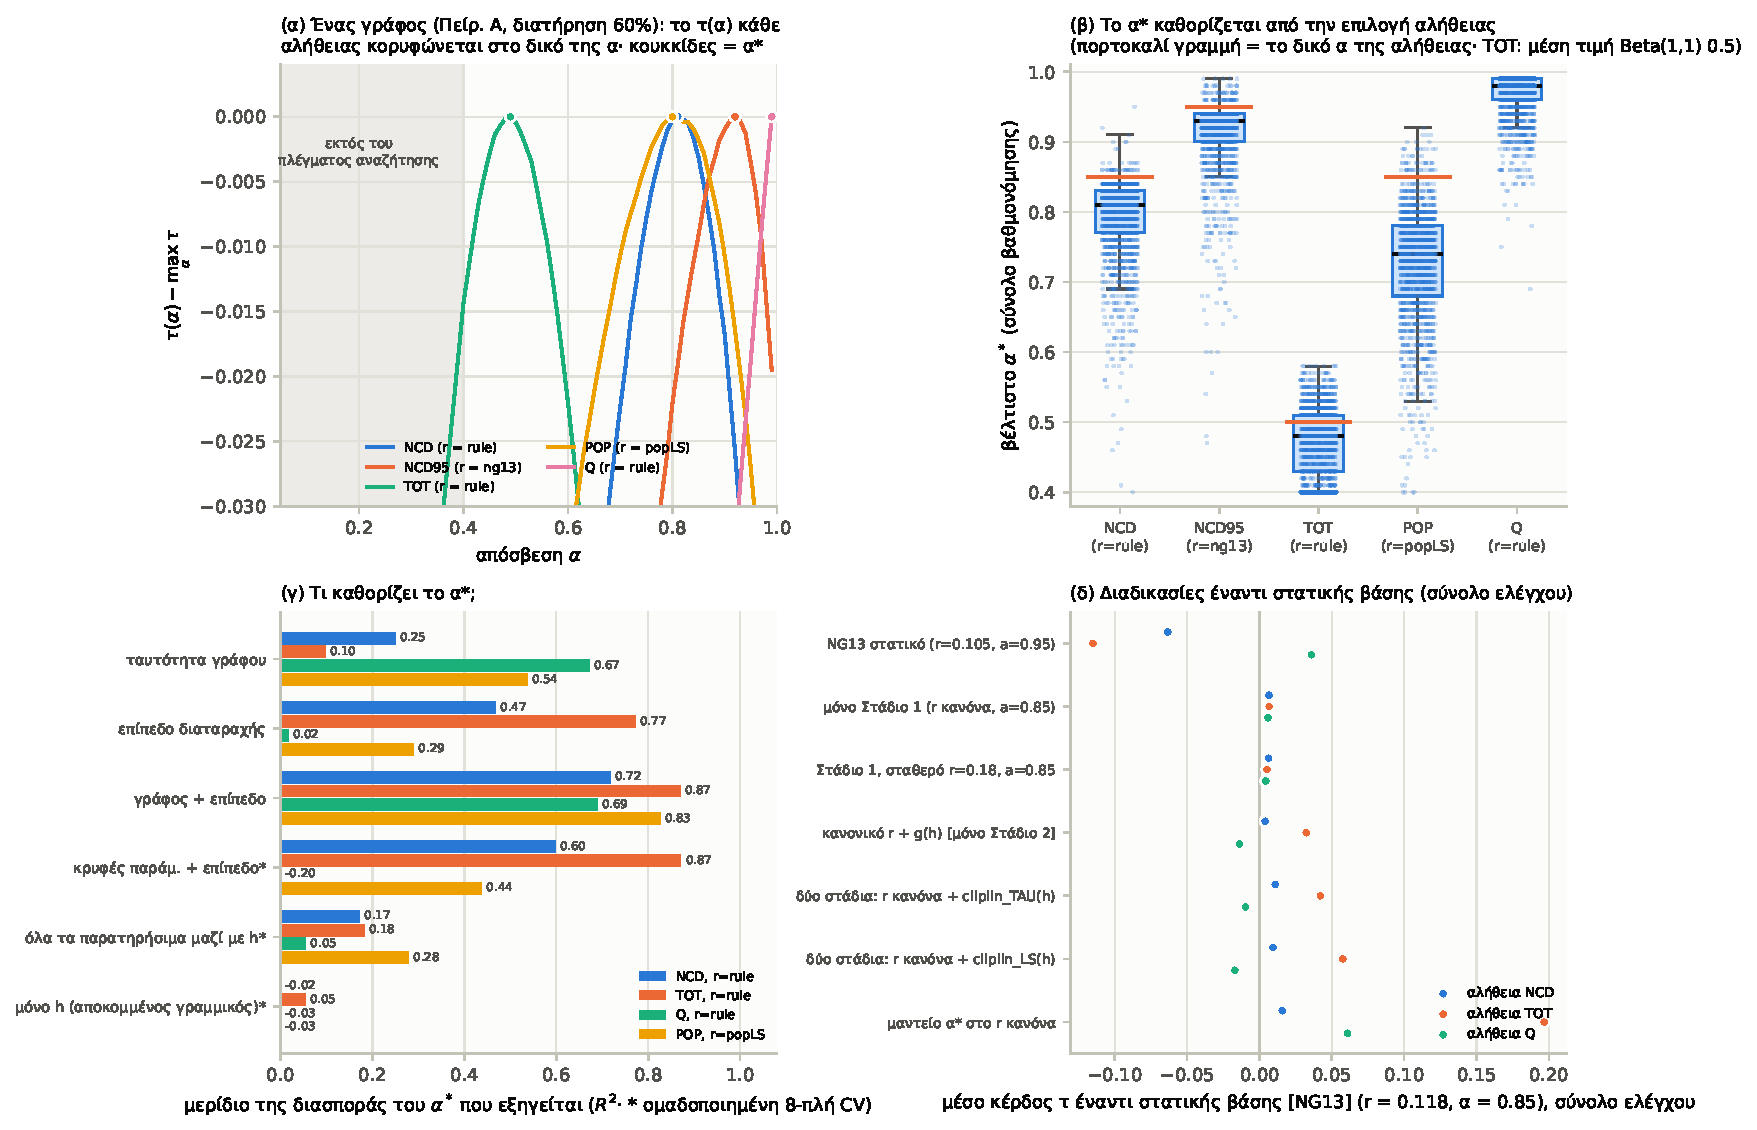
\includegraphics[width=\textwidth]{stage2_diagnostics.pdf}
\caption{Διαγνωστικά του Σταδίου~2. \textbf{(α)} Για έναν γράφο βαθμονόμησης (Πείραμα~Α, διατήρηση του
$60\%$ των τόξων), η καμπύλη $\tau(\alpha)-\max\tau$ υπό κάθε αλήθεια κορυφώνεται κοντά στην απόσβεση
που ορίζει την αλήθεια αυτή. \textbf{(β)} Κατανομή του $\alpha^*$ ανά αλήθεια· οι πορτοκαλί γραμμές
σημειώνουν το δικό $\alpha$ κάθε αλήθειας. \textbf{(γ)} Μερίδιο της διασποράς του $\alpha^*$ που
εξηγείται. \textbf{(δ)} Κέρδος έναντι της στατικής ρύθμισης $(0.118,0.85)$ στο \texttt{test} για
πλήρεις διαδικασίες υπό τρεις αλήθειες. Το πρόσημο του κέρδους της διαδικασίας δύο σταδίων
αντιστρέφεται από αλήθεια σε αλήθεια.}
\label{fig:s2diag}
\end{figure}

\begin{figure}[t]
\centering
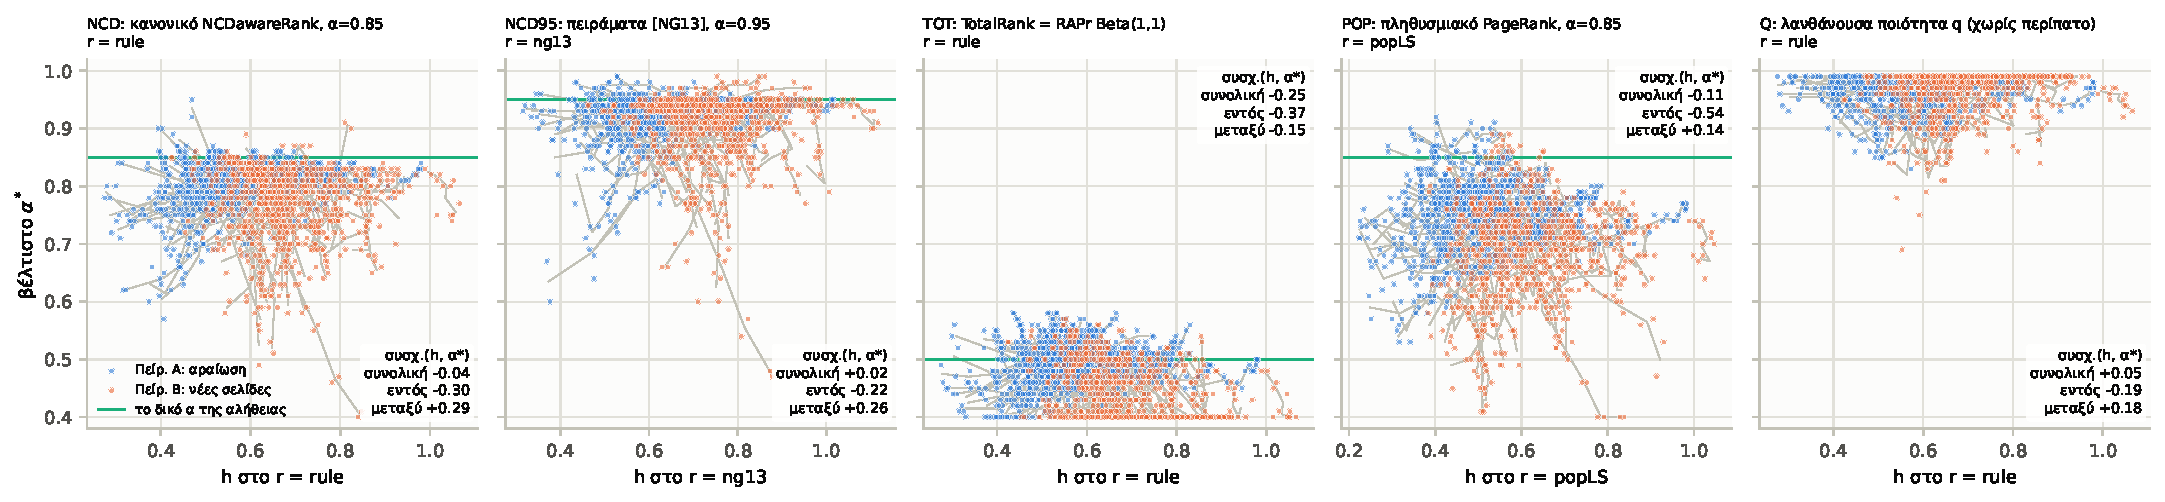
\includegraphics[width=\textwidth]{stage2_gt_sensitivity.pdf}
\caption{Βέλτιστη απόσβεση έναντι του $h$ υπό τις πέντε αλήθειες (σύνολο βαθμονόμησης). Εντός κάθε
αλήθειας η σχέση με το $h$ είναι ασθενής και μεικτού προσήμου· μεταξύ αληθειών το επίπεδο του
$\alpha^*$ ακολουθεί την απόσβεση που ορίζει την αλήθεια (πράσινη γραμμή).}
\label{fig:s2truth}
\end{figure}

\subsection{Πλήρεις διαδικασίες έναντι των στατικών ρυθμίσεων}
Ο Πίνακας~\ref{tab:pipe} συγκρίνει πλήρεις διαδικασίες $(r,\alpha)$ με τις δύο δημοσιευμένες στατικές
ρυθμίσεις, υπό και τις πέντε αλήθειες και σε όλα τα σύνολα. Υπό την κύρια αλήθεια, η διαδικασία δύο
σταδίων (κλειδωμένος κανόνας για το $r$, $\alpha=\STwoConstAlpha$) βελτιώνει την κανονική ρύθμιση
$(0.118,0.85)$ κατά \TwoTestD{} στο \texttt{test} (95\% ΔΕ $[\TwoTestLo,\TwoTestHi]$, καλύτερη σε
\TwoTestWins{} γράφους, $p=\TwoTestP$), \TwoScaleD{} στο \texttt{scale} (\TwoScaleWins) και \TwoTopoD{}
στο \texttt{topo} (\TwoTopoWins). Αυτό αντιστοιχεί περίπου στα δύο τρίτα του περιθωρίου του μαντείου
στο \texttt{test} (\PipeNcdOracleVsLoTest). Το κέρδος αναλύεται σε \StoTestD{} από το Στάδιο~1
($p=\StoTestP$) και \SthTestD{} από το Στάδιο~2 ($p=\SthTestP$). Στο \texttt{real} είναι \TwoRealD{} ανά
γράφο (95\% ΔΕ $[\TwoRealLo,\TwoRealHi]$, \TwoRealWins{} γράφοι, $p=\TwoRealP$): \TwoRealCnr{} στο
cnr-2000, \TwoRealCorafull{} στο Cora, \TwoRealCiteseer{} στο CiteSeer, \TwoRealCoraml{} στο Cora-ML και
\TwoRealWikics{} στο WikiCS (Πίνακας~\ref{tab:realdetail} του Παραρτήματος).

Η ετυμηγορία εξαρτάται από την αλήθεια (Σχήμα~\ref{fig:s2diag}(δ)). Η ίδια κλειδωμένη διαδικασία:
\begin{itemize}[leftmargin=1.4em,itemsep=0pt]
\item υπερέχει της κανονικής ρύθμισης υπό την TOT (\PipeTotTwoVsLoTest) και την POP
(\PipePopTwoVsLoTest), απλώς επειδή το $0.81$ βρίσκεται πλησιέστερα από το $0.85$ στις άγκυρες αυτών
των αληθειών·
\item υστερεί έναντι της ρύθμισης $(0.105,0.95)$ του~\cite{ng13} υπό την NCD95 (\PipeNcdnfTwoVsHiTest)
και υπό την ανεξάρτητη από περιπάτους Q (\PipeQTwoVsHiTest), των οποίων οι άγκυρες βρίσκονται πάνω από
$0.9$.
\end{itemize}
Οι ισχυρισμοί ότι μια βαθμονομημένη απόσβεση «υπερέχει της προεπιλογής» είναι επομένως ισχυρισμοί τόσο
για την αναφορά όσο και για τη μέθοδο.

\begin{table*}[t]
\centering
\scriptsize
\caption{Πλήρεις διαδικασίες έναντι των στατικών ρυθμίσεων του [NG13] υπό και τις πέντε αλήθειες. Κελιά: μέσο $\tau$ του Kendall ανά στιγμιότυπο· σε παρένθεση, η διαφορά έναντι του [NG13] $(0.118,0.85)$ με μέσο όρο ανά γράφο (κάθε γράφος με ίσο βάρος). \emph{Δύο στάδια}: $r$ από τον κλειδωμένο κανόνα του Σταδίου~1 και $\alpha=0.81$, αμφότερα προσαρμοσμένα σε γράφους βαθμονόμησης υπό NCD και εφαρμοσμένα αμετάβλητα υπό κάθε αλήθεια. Οι αλήθειες POP και Q υπάρχουν μόνο για τη στατική γεννήτρια.}
\label{tab:pipe}
\begin{tabular}{@{}lccccc@{}}
\toprule
πολιτική $(r,\alpha)$ & \texttt{calib} & \texttt{test} & \texttt{scale} & \texttt{topo} & \texttt{real} \\
\midrule
\multicolumn{6}{@{}l}{\textit{αλήθεια NCD}} \\
\quad [NG13] $(0.118,\,0.85)$ & 0.6805 & 0.6801 & 0.6633 & 0.7840 & 0.7559 \\
\quad [NG13] $(0.105,\,0.95)$ & 0.6133 ($-$0.0673) & 0.6168 ($-$0.0633) & 0.5979 ($-$0.0654) & 0.7360 ($-$0.0479) & 0.6792 ($-$0.0831) \\
\quad μόνο Στάδιο 1 & 0.6862 ($+$0.0056) & 0.6867 ($+$0.0066) & 0.6681 ($+$0.0049) & 0.7844 ($+$0.0005) & 0.7600 ($+$0.0030) \\
\quad δύο στάδια ($\alpha=0.81$) & 0.6913 ($+$0.0108) & 0.6911 ($+$0.0110) & 0.6735 ($+$0.0102) & 0.7875 ($+$0.0036) & 0.7559 ($+$0.0017) \\
\quad μαντείο $\alpha^*$ & 0.6965 ($+$0.0160) & 0.6960 ($+$0.0159) & 0.6787 ($+$0.0155) & 0.7911 ($+$0.0071) & 0.7738 ($+$0.0189) \\
\multicolumn{6}{@{}l}{\textit{αλήθεια NCD95}} \\
\quad [NG13] $(0.118,\,0.85)$ & 0.6227 & 0.6237 & 0.6044 & 0.7472 & 0.6678 \\
\quad [NG13] $(0.105,\,0.95)$ & 0.6410 ($+$0.0182) & 0.6431 ($+$0.0194) & 0.6226 ($+$0.0183) & 0.7576 ($+$0.0104) & 0.7122 ($+$0.0449) \\
\quad μόνο Στάδιο 1 & 0.6282 ($+$0.0055) & 0.6306 ($+$0.0069) & 0.6096 ($+$0.0052) & 0.7472 ($-$0.0001) & 0.6767 ($+$0.0104) \\
\quad δύο στάδια ($\alpha=0.81$) & 0.6103 ($-$0.0125) & 0.6128 ($-$0.0109) & 0.5920 ($-$0.0124) & 0.7404 ($-$0.0069) & 0.6463 ($-$0.0206) \\
\quad μαντείο $\alpha^*$ & 0.6530 ($+$0.0303) & 0.6560 ($+$0.0323) & 0.6343 ($+$0.0299) & 0.7660 ($+$0.0188) & 0.7281 ($+$0.0609) \\
\multicolumn{6}{@{}l}{\textit{αλήθεια TOT}} \\
\quad [NG13] $(0.118,\,0.85)$ & 0.5893 & 0.5932 & 0.5773 & 0.7624 & 0.6804 \\
\quad [NG13] $(0.105,\,0.95)$ & 0.4689 ($-$0.1204) & 0.4782 ($-$0.1150) & 0.4591 ($-$0.1183) & 0.7001 ($-$0.0623) & 0.5387 ($-$0.1461) \\
\quad μόνο Στάδιο 1 & 0.5963 ($+$0.0071) & 0.6000 ($+$0.0068) & 0.5854 ($+$0.0080) & 0.7655 ($+$0.0030) & 0.6688 ($-$0.0128) \\
\quad δύο στάδια ($\alpha=0.81$) & 0.6341 ($+$0.0449) & 0.6354 ($+$0.0422) & 0.6230 ($+$0.0457) & 0.7775 ($+$0.0151) & 0.7097 ($+$0.0298) \\
\quad μαντείο $\alpha^*$ & 0.7987 ($+$0.2094) & 0.7899 ($+$0.1967) & 0.7839 ($+$0.2065) & 0.8094 ($+$0.0469) & 0.8336 ($+$0.1582) \\
\multicolumn{6}{@{}l}{\textit{αλήθεια POP}} \\
\quad [NG13] $(0.118,\,0.85)$ & 0.5462 & 0.5446 & 0.5172 & -- & -- \\
\quad [NG13] $(0.105,\,0.95)$ & 0.4904 ($-$0.0558) & 0.4957 ($-$0.0490) & 0.4683 ($-$0.0489) & -- & -- \\
\quad μόνο Στάδιο 1 & 0.5510 ($+$0.0048) & 0.5506 ($+$0.0060) & 0.5237 ($+$0.0065) & -- & -- \\
\quad δύο στάδια ($\alpha=0.81$) & 0.5614 ($+$0.0152) & 0.5585 ($+$0.0139) & 0.5326 ($+$0.0154) & -- & -- \\
\quad μαντείο $\alpha^*$ & 0.5745 ($+$0.0283) & 0.5677 ($+$0.0231) & 0.5443 ($+$0.0271) & -- & -- \\
\multicolumn{6}{@{}l}{\textit{αλήθεια Q}} \\
\quad [NG13] $(0.118,\,0.85)$ & 0.3655 & 0.3478 & 0.3302 & -- & -- \\
\quad [NG13] $(0.105,\,0.95)$ & 0.3939 ($+$0.0283) & 0.3837 ($+$0.0359) & 0.3560 ($+$0.0258) & -- & -- \\
\quad μόνο Στάδιο 1 & 0.3724 ($+$0.0069) & 0.3537 ($+$0.0059) & 0.3332 ($+$0.0030) & -- & -- \\
\quad δύο στάδια ($\alpha=0.81$) & 0.3585 ($-$0.0070) & 0.3382 ($-$0.0096) & 0.3202 ($-$0.0100) & -- & -- \\
\quad μαντείο $\alpha^*$ & 0.4150 ($+$0.0495) & 0.4087 ($+$0.0609) & 0.3712 ($+$0.0410) & -- & -- \\
\bottomrule
\end{tabular}
\end{table*}


\subsection{Σύγκλιση}
Η μείωση του $\alpha$ συντομεύει επίσης τη μέθοδο των δυνάμεων. Αυτό ισχύει για οποιοδήποτε μικρότερο
$\alpha$ και αποτελεί παράπλευρο όφελος, όχι ιδιότητα της βαθμονόμησης. Η εκ των προτέρων εκτίμηση
$k\approx\ln\varepsilon/\ln\alpha$, βασισμένη στο $|\lambda_2(P)|\le\alpha$~\cite{haveliwala03,ng13},
προβλέπει εξοικονόμηση \ConvNcdBound\% για $0.85\to0.81$ ($\ConvNcdBoundK$ επαναλήψεις για
$\varepsilon=10^{-6}$) και \ConvNfBound\% για $0.95\to0.93$. Η μετρημένη εξοικονόμηση είναι μικρότερη.
Η πραγματική συστολή είναι ταχύτερη από το $\alpha$, οπότε και οι δύο αριθμοί επαναλήψεων παραμένουν
αρκετά κάτω από την εκτίμηση (Πίνακας~\ref{tab:conv}), και η εξοικονόμηση είναι \ConvNcdTest\% στο
\texttt{test} και \ConvNcdReal\% στο \texttt{real} για τον κλάδο NCD, και \ConvNfTest\% και
\ConvNfReal\% για τον κλάδο NCD95.

\begin{table*}[t]
\centering
\small
\caption{Πλήθος επαναλήψεων της μεθόδου δυνάμεων πριν και μετά την έκπτωση θορύβου (κριτήριο τερματισμού $\|\pi^{(k+1)}-\pi^{(k)}\|_1<\varepsilon=10^{-6}$, αρχή $v$). Η στήλη του φράγματος είναι η εκ των προτέρων εκτίμηση από το $|\lambda_2(P)|\le\alpha$· οι μετρημένες στήλες είναι μέσοι όροι σε όλα τα διαταραγμένα στιγμιότυπα του συνόλου.}
\label{tab:conv}
\begin{tabular}{@{}lllll@{}}
\toprule
διάταξη & $\alpha$ & φράγμα $\ln\varepsilon/\ln\alpha$ & μετρημένο, \texttt{test} & μετρημένο, \texttt{real} \\
\midrule
κλάδος NCD ($r$ = κανόνας) & 0.85$\to$0.81 & 85$\to$66 ($-22.9\%$) & 30.2$\to$25.8 ($-14.7\%$) & 30.5$\to$26.5 ($-13.1\%$) \\
κλάδος NCD95 ($r=0.105$) & 0.95$\to$0.93 & 269$\to$190 ($-29.3\%$) & 67.2$\to$54.2 ($-19.3\%$) & 69.9$\to$59.2 ($-15.3\%$) \\
\bottomrule
\end{tabular}
\end{table*}


\subsection{Αλήθειες ευαισθησίας με επαναπροσαρμοσμένους κανόνες}
Η επαναπροσαρμογή της $g$ χωριστά για κάθε αλήθεια δεν αλλάζει το συμπέρασμα
(Πίνακας~\ref{tab:sens} του Παραρτήματος). Υπό τις Q, POP και NCD95, ο βέλτιστος ως προς $\tau$ κανόνας
στο $h$ είναι η σταθερά ή αδιάκριτος από αυτήν. Υπό την TOT, το $h$ φέρει ένα ασθενές σήμα με το ίδιο
αρνητικό πρόσημο εντός και μεταξύ γράφων. Κερδίζει \TotHTest{} στο \texttt{test} ($p=\TotHTestP$),
αλλά \TotHTopo{} στο \texttt{topo} και \TotHReal{} στο \texttt{real}, οπότε δεν μεταφέρεται.

\FloatBarrier
% =============================================================================
\section{Επέκταση V2: εξωτερικοί πραγματικοί γράφοι και επιχειρησιακοί έλεγχοι}
\label{sec:v2extension}

Η προεγγεγραμμένη συνενωμένη ανάλυση real2 συνδυάζει τους πέντε παλαιούς πραγματικούς
γράφους με τους έξι νέους, με μονάδες αναπαραγωγής τους γράφους
($n=\VTwoRealN$). Η H1 είναι \VTwoRealHone{} (\VTwoRealHoneWins{}, $p=\VTwoRealHoneP$)
και η H3b είναι \VTwoRealHthree{} (\VTwoRealHthreeWins{}, $p=\VTwoRealHthreeP$).
Η H2 είναι \VTwoRealHtwo{} (\VTwoRealHtwoWins{}, $p=\VTwoRealHtwoP$), αλλά συγκρίνει
διαφορετικές άγκυρες και είναι μόνο περιγραφική. Η οικογένεια Holm των έξι νέων
γράφων δεν μπορεί να ελεγχθεί σύμφωνα με την Τροποποίηση~1. Ο Cornell είναι
καθοριστικός (\VTwoCornellN{} κόμβοι, \VTwoCornellM{} τόξα, \VTwoCornellDang{} κρεμάμενοι·
κέρδος H1 \VTwoCornellHone{}).
Οι ετικέτες είναι υποκατάστατα θεματικής ή τμηματικής δομής και οι διαμερίσεις
SNAP υποκατάστατα φιλοξενητών· συνεπώς δεν υποστηρίζεται γενίκευση του κέρδους
σε νέους πραγματικούς γράφους.

\begin{table*}[t]
\centering
\scriptsize
\caption{Μέσοι όροι ανά γράφο για H1, H2 και H3b στη συνενωμένη real2 ανάλυση. Η H2 έχει ασυμφωνία άγκυρας και είναι περιγραφική· η συνενωμένη επαγωγική ανάλυση έχει 11 γράφους.}
\label{tab:v2real2}
\begin{tabular}{@{}lllrrr@{}}\toprule
γράφος & ομάδα & διαμέριση & H1 & H2 & H3b \\
\midrule
citeseer & old & label & -0.0024 & +0.0636 & -0.0092 \\
cnr2000 & old & proxy & +0.0172 & +0.1578 & +0.0072 \\
cora\_full & old & label & +0.0020 & +0.0923 & -0.0008 \\
cora\_ml & old & label & -0.0032 & +0.0554 & -0.0029 \\
wikics & old & label & -0.0049 & +0.0550 & -0.0067 \\
cornell & new & label & -0.0355 & +0.0699 & -0.0061 \\
email-Eu-core & new & label & -0.0052 & +0.0566 & -0.0067 \\
film & new & label & -0.0012 & +0.0238 & -0.0005 \\
ogbn-arxiv & new & label & +0.0128 & +0.1826 & +0.0030 \\
texas & new & label & +0.0012 & +0.0439 & -0.0156 \\
web-NotreDame & new & proxy & -0.0235 & -0.0301 & -0.0118 \\
web-Stanford & new & proxy & +0.0026 & +0.0186 & +0.0028 \\
wisconsin & new & label & -0.0044 & +0.0353 & -0.0026 \\
\bottomrule\end{tabular}
\end{table*}


Η επιχειρησιακή έκπτωση άγκυρας δεν προάγεται. Κερδίζει
\VTwoAnchorTest{} στο \texttt{test}, \VTwoAnchorTopo{} στο \texttt{topo} και
\VTwoAnchorReal{} στο \texttt{real}· η απώλεια στο \texttt{topo} είναι σημαντική
και το συνενωμένο αποτέλεσμα εκτός δείγματος αποτυγχάνει το προεγγεγραμμένο όριο.
\begin{table}[t]
\centering
\small
\caption{Τυπικά αποτελέσματα του κανόνα απόφασης για την έκπτωση άγκυρας έναντι μηδενικής έκπτωσης.}
\label{tab:v2anchor}
\begin{tabular}{@{}lrrrr@{}}\toprule
σύγκριση & μέση διαφορά & νίκες/$n$ & ακριβές $p$ & bootstrap 95\% ΔΕ \\
\midrule
calib CV & +0.0031 & 45/64 & 0.0000 & [+0.0020, +0.0042] \\
pooled held-out & -0.0005 & 22/61 & 0.0646 & [-0.0018, +0.0008] \\
test & -0.0008 & 14/32 & 0.3217 & [-0.0026, +0.0013] \\
topo & -0.0004 & 6/24 & 0.0340 & [-0.0013, +0.0007] \\
real & +0.0002 & 2/5 & 1.0000 & [-0.0086, +0.0091] \\
\bottomrule\end{tabular}
\end{table}


Η αντίθεση μικτής ζημιάς ανά γράφο δεν προάγει τα C4--C7 έναντι του C1.
\begin{table}[t]
\centering
\small
\caption{Αντίθεση μικτής ζημιάς ανά γράφο στα σύνολα εκτός δείγματος έναντι του C1· κανένας κανόνας δεν προάγεται.}
\label{tab:v2mixed}
\begin{tabular}{@{}lrrrr@{}}\toprule
κανόνας & γράφοι & μέση διαφορά έναντι C1 & νίκες & ακριβές $p$ \\
\midrule
C4 & 36 & -0.0003 & 22 & 0.3074 \\
C5 & 36 & -0.0024 & 15 & 0.1079 \\
C6 & 36 & +0.0002 & 13 & 0.0395 \\
C7 & 36 & -0.0012 & 13 & 0.0334 \\
\bottomrule\end{tabular}
\end{table}

Τα πλήρη πάνελ baseline B1--B3 παραμένουν μόνο περιγραφικά: οι μέσες
διαφορές ήταν \VTwoBOneMean{}, \VTwoBTwoMean{} και \VTwoBThreeMean{}
αντίστοιχα· κανένας κανόνας baseline δεν προάγεται.

\FloatBarrier
% =============================================================================
\section{Συζήτηση}
\label{sec:discussion}

\paragraph{Τι επιτυγχάνει η βαθμονόμηση.} Έναντι της κανονικής αναφοράς, η διαδικασία δύο σταδίων
ισοδυναμεί με επαναρρύθμιση δύο σταθερών: μεγαλύτερο βάρος στον πίνακα εγγύτητας ($r\approx0.2$,
$\mu\approx0.17$ αντί για $0.10$) και ελαφρώς μικρότερη απόσβεση ($\alpha=\STwoConstAlpha$ αντί για
$0.85$). Σε συνθετικούς γράφους εκτός δείγματος, μεταξύ των οποίων μεγαλύτεροι γράφοι και ένας
διαφορετικός γενετικός μηχανισμός, το κέρδος είναι $0.004$--$0.011$ στο $\tau$ του Kendall, σταθερό
από γράφο σε γράφο, συν μια μέτρια επιτάχυνση. Στους συνενωμένους παλαιούς και νέους πραγματικούς
γράφους η H1 είναι σχεδόν μηδενική και η H3b ελαφρώς αρνητική· δεν υποστηρίζεται γενίκευση του
κέρδους σε νέους πραγματικούς γράφους. Πρόκειται για έντιμα, αν και μέτρια, αποτελέσματα για μια διαδικασία μηδενικού κόστους. Δεν
πρόκειται για την προσαρμοστική, καθοδηγούμενη από τη δομή βαθμονόμηση που υποκίνησε τη μελέτη.

\paragraph{Γιατί αποτυγχάνουν εδώ τα δομικά στατιστικά.} Οι βέλτιστες παράμετροι εξαρτώνται από δύο
μεγέθη: πόσο έντονα είναι διαταραγμένος ο παρατηρούμενος γράφος σε σχέση με την αναφορά, και τη
λανθάνουσα δομή ποιότητας των σελίδων. Κανένα από τα δύο δεν αποκαλύπτεται από καθολικά στατιστικά του
παρατηρούμενου γράφου. Τα $\Pbar$ και $h$ αντιδρούν έντονα στην απώλεια συνδέσμων εντός ενός γράφου.
Μεταξύ γράφων, τα επίπεδά τους συγχέονται με τη συνήθη δομική μεταβλητότητα, και το $h$ αποκρίνεται σε
διαφορετικά είδη απώλειας συνδέσμων με αντίθετα πρόσημα. Η Ενότητα~\ref{sec:hmech} απομονώνει το
συστατικό που λείπει: αν είναι γνωστή η τιμή $h_0$ του αδιατάρακτου γράφου, μια τέντα στο $h-h_0$
ανακτά το \NmDhShare\% του περιθωρίου του μαντείου στη διασταυρωμένη επικύρωση, ενώ κανένας από τους
\NmRules{} κανόνες σε στατιστικά μόνο του παρατηρούμενου γράφου δεν περνά τον έλεγχο εκτός δείγματος.
Το στατιστικό θα μπορούσε επομένως να φανεί χρήσιμο όπου υπάρχει ως αναφορά ένα λιγότερο διαταραγμένο
στιγμιότυπο του ίδιου γράφου· αυτό δεν το έχουμε ελέγξει.
Ένα συγγενές μοτίβο εμφανίστηκε στην
προηγούμενη εργασία μας σε αβέβαιους γράφους~\cite{konstantellos26}: εκεί, η συσχέτιση της πιθανότητας
διαφυγής με τη βέλτιστη απόσβεση δεν επιβίωσε στα πραγματικά δίκτυα, και η δρομολόγηση μεταξύ ευρετικών
με βάση το ίδιο στατιστικό λειτούργησε στους συνθετικούς γράφους αλλά απέτυχε στους πραγματικούς. Το
θεωρούμε ένδειξη ότι μεμονωμένα καθολικά στατιστικά είναι πολύ αδρά για να μεταφέρουν επιλογές
παραμέτρων από γράφο σε γράφο.

\paragraph{Η αγκύρωση ως μεθοδολογικό δίδαγμα.} Το ισχυρότερο εύρημα δεν αφορά το NCDawareRank. Όταν
μια μέθοδος κατάταξης ρυθμίζεται ώστε να συμφωνεί με μια κατάταξη αναφοράς, η βέλτιστη απόσβεση είναι η
απόσβεση της ίδιας της αναφοράς μείον μια έκπτωση θορύβου. Αυτό προκύπτει από τον έλεγχο
δόσης--απόκρισης και από πέντε αλήθειες με πολύ διαφορετικές άγκυρες. Κάθε δήλωση ότι ένας συντελεστής
απόσβεσης είναι «καλύτερος» κληρονομεί επομένως την απόσβεση της αλήθειας αναφοράς. Οι δύο αναφορές
ανεξάρτητες από το $\alpha$ που έχουμε στη διάθεσή μας διαφέρουν σχεδόν κατά $0.5$, γεγονός που
υποδηλώνει ότι δεν υπάρχει βέλτιστη απόσβεση ανεξάρτητη από την αλήθεια για αυτό το πρόβλημα. Οι
αξιολογήσεις επιλογών απόσβεσης θα πρέπει να αναφέρουν αποτελέσματα υπό πολλές αναφορές, και τα
πρωτόκολλα σταθερότητας δεν θα πρέπει να χρησιμοποιούνται για την επιλογή παραμέτρων.

\paragraph{Τι προσφέρει η θεωρία του $h$.} Οι ταυτότητες της Πρότασης~\ref{prop:interp} και το φράγμα
του Θεωρήματος~\ref{thm:bound} δίνουν στα $h$ και $h_v$ ακριβές νόημα: μετρούν πόσο ισχυρά ωθεί η
αλυσίδα τη βαθμολογία μακριά από την ομοιόμορφη κατανομή και από την κατανομή τηλεμεταφοράς, και το
$h_v$ φράσσει τη συνολική μετατόπιση της κατάταξης για κάθε $\alpha$. Είναι χρήσιμα διαγνωστικά, για
παράδειγμα για να κριθεί αν η απόσβεση έχει καν σημασία για έναν δεδομένο γράφο. Τα εμπειρικά
αποτελέσματα δείχνουν ότι δεν είναι στατιστικά βαθμονόμησης.

\paragraph{Περιορισμοί.} Οι συνθετικές γεννήτριες, όσο ποικίλες κι αν είναι, είναι δικές μας. Η
διαμέριση του cnr-2000 είναι προσέγγιση hosts, οι γράφοι παραπομπών χρησιμοποιούν θεματικές
ετικέτες, και οι νέες ετικέτες και διαμερίσεις SNAP είναι υποκατάστατα. Ο Cornell επηρεάζει ουσιαστικά
την H1. Οι κρεμάμενες σελίδες αντιμετωπίζονται με ομοιόμορφες γραμμές και όχι με τη
στρατηγική περιορισμού εντός του μπλοκ του~\cite{ng20}. Το Στάδιο~1 είναι αγκυρωμένο στο $\alpha_0=0.85$,
και το πλέγμα του Σταδίου~2 σταματά στο $0.99$, γεγονός που λογοκρίνει (censoring) το μαντείο υπό την Q
(ελέγξαμε ότι το βέλτιστο δεν βρίσκεται πέρα από αυτό). Αξιολογούμε μόνο συσχετίσεις κατατάξεων, έναντι
αναφορών που προκύπτουν από μοντέλα. Εξωτερικές κρίσεις συνάφειας ή δεδομένα περιήγησης, όπως
στο~\cite{gleich10}, θα παρείχαν μια αλήθεια αναφοράς που δεν εξαρτάται από κάποιον συντελεστή
απόσβεσης.

% =============================================================================
\section{Συμπεράσματα}
\label{sec:conclusion}

Διατυπώσαμε μια βαθμονόμηση δύο σταδίων μηδενικού κόστους για το NCDawareRank. Ο λόγος ανάμειξης
προκύπτει από την πιθανότητα διαφυγής από το μπλοκ και η συνολική απόσβεση από την απόκλιση του
συνδυασμένου τελεστή από τη διπλή στοχαστικότητα. Αποδείξαμε ταυτότητες και ένα φράγμα μετατόπισης που
δίνουν στα στατιστικά αυτά ακριβές νόημα. Μια εκτενής αξιολόγηση που λαμβάνει υπόψη τις συστάδες δείχνει
ότι τα στατιστικά δεν προβλέπουν τις βέλτιστες παραμέτρους. Η βαθμονόμηση ανάγεται σε δύο σταθερές,
$r\approx0.2$ και $\alpha=\STwoConstAlpha$, που βελτιώνουν την ανάκτηση της κανονικής κατάταξης στους
συνθετικούς γράφους κατά $0.004$--$0.011$ στο $\tau$ του Kendall και δεν γενικεύουν ως κέρδος στους
συνενωμένους πραγματικούς γράφους. Η βέλτιστη απόσβεση είναι αγκυρωμένη στην απόσβεση της κατάταξης αναφοράς, μείον μια έκπτωση
θορύβου. Η επιλογή της αλήθειας αναφοράς καθορίζει επομένως ποια ρύθμιση παραμέτρων υπερισχύει, και
συνιστούμε οι μελλοντικές συγκρίσεις παραμέτρων ανάλυσης συνδέσμων να αναφέρουν αποτελέσματα υπό
πολλές αναφορές.

\section*{Αναπαραγωγιμότητα}
Όλος ο κώδικας, τα πρωτογενή αποτελέσματα και τα σχήματα συνοδεύουν την εργασία· η συνοδευτική
τεκμηρίωση περιγράφει κάθε άρθρωμα. Συνοπτικά:
\begin{itemize}[leftmargin=1.4em,itemsep=0pt]
\item το \texttt{prepare\_real\_graphs.py} κατασκευάζει το σύνολο των πραγματικών δικτύων·
\item τα \texttt{run\_experiments.py stage1} και \texttt{run\_experiments.py stage2} εκτελούν τα δύο
στάδια·
\item τα \texttt{stage1\_analysis.py}, \texttt{stage2\_analysis.py} και τα σενάρια αποσύνθεσης,
αγκύρωσης, σύγκλισης και ελέγχου του φράγματος παράγουν κάθε αριθμό·
\item το \texttt{make\_paper\_assets.py} γράφει τους αριθμούς και τους πίνακες του κειμένου απευθείας
από τα αρχεία αποτελεσμάτων.
\end{itemize}
Έλεγχοι μονάδας επαληθεύουν την υλοποίηση έναντι των πινάκων του~\cite[Σχ.~1]{ng13}, των
Θεωρημάτων~1--2 του~\cite{ng13}, πυκνών επιλύσεων, αριθμητικής ολοκλήρωσης και του
φράγματος~\eqref{eq:bound}.

% =============================================================================
\begin{otherlanguage}{english}
\renewcommand{\refname}{Βιβλιογραφία}
\begin{thebibliography}{PBMW99}
\raggedright
\small
\bibitem[ALP08]{avrachenkov08} K.~Avrachenkov, N.~Litvak, K.~S.~Pham. A singular perturbation approach for
choosing the PageRank damping factor. \emph{Internet Mathematics}, 5(1--2):47--69, 2008.
\bibitem[BBC06]{baeza06} R.~Baeza-Yates, P.~Boldi, C.~Castillo. Generic damping functions for propagating
importance in link-based ranking. \emph{Internet Mathematics}, 3(4):445--478, 2006.
\bibitem[BCSV04]{boldi04ubi} P.~Boldi, B.~Codenotti, M.~Santini, S.~Vigna. UbiCrawler: a scalable fully
distributed Web crawler. \emph{Software: Practice and Experience}, 34(8):711--726, 2004.
\bibitem[BG18]{bojchevski18} A.~Bojchevski, S.~G\"unnemann. Deep Gaussian embedding of graphs: unsupervised
inductive learning via ranking. In \emph{Proc.\ ICLR}, 2018.
\bibitem[BNG19]{berberidis19} D.~Berberidis, A.~N.~Nikolakopoulos, G.~B.~Giannakis. Adaptive diffusions for
scalable learning over graphs. \emph{IEEE Trans.\ Signal Processing}, 67(5):1307--1321, 2019.
\bibitem[Bol05]{boldi05tr} P.~Boldi. TotalRank: ranking without damping. In \emph{Special Interest Tracks and
Posters of the 14th WWW}, 898--899, 2005.
\bibitem[BP10]{bressan10} M.~Bressan, E.~Peserico. Choose the damping, choose the ranking? \emph{J.\ Discrete
Algorithms}, 8(2):199--213, 2010.
\bibitem[BSV05]{boldi05} P.~Boldi, M.~Santini, S.~Vigna. PageRank as a function of the damping factor. In
\emph{Proc.\ 14th WWW}, 557--566, 2005.
\bibitem[BSV09]{boldi09} P.~Boldi, M.~Santini, S.~Vigna. PageRank: functional dependencies. \emph{ACM Trans.\
Information Systems}, 27(4):19, 2009.
\bibitem[BV04]{boldi04} P.~Boldi, S.~Vigna. The WebGraph framework I: compression techniques. In \emph{Proc.\
13th WWW}, 595--602, 2004.
\bibitem[CG09]{constantine09} P.~G.~Constantine, D.~F.~Gleich. Random alpha PageRank. \emph{Internet
Mathematics}, 6(2):189--236, 2009.
\bibitem[Cou77]{courtois77} P.-J.~Courtois. \emph{Decomposability: Queueing and Computer System Applications}.
Academic Press, 1977.
\bibitem[ET93]{efron93} B.~Efron, R.~J.~Tibshirani. \emph{An Introduction to the Bootstrap}. Chapman \& Hall,
1993.
\bibitem[FBFM08]{fortunato08} S.~Fortunato, M.~Bogu\~n\'a, A.~Flammini, F.~Menczer. Approximating PageRank from
in-degree. In \emph{Algorithms and Models for the Web-Graph (WAW 2006)}, LNCS 4936, 59--71, 2008.
\bibitem[Fri01]{friedman01} J.~H.~Friedman. Greedy function approximation: a gradient boosting machine.
\emph{Annals of Statistics}, 29(5):1189--1232, 2001.
\bibitem[GCFG10]{gleich10} D.~F.~Gleich, P.~G.~Constantine, A.~D.~Flaxman, A.~Gunawardana. Tracking the random
surfer: empirically measured teleportation parameters in PageRank. In \emph{Proc.\ 19th WWW}, 381--390,
2010.
\bibitem[HK03]{haveliwala03} T.~H.~Haveliwala, S.~D.~Kamvar. The second eigenvalue of the Google matrix.
Technical Report 2003-20, Stanford InfoLab, 2003.
\bibitem[Ken38]{kendall38} M.~G.~Kendall. A new measure of rank correlation. \emph{Biometrika}, 30(1/2):81--93,
1938.
\bibitem[Ken45]{kendall45} M.~G.~Kendall. The treatment of ties in ranking problems. \emph{Biometrika},
33(3):239--251, 1945.
\bibitem[KH03]{kamvar03} S.~D.~Kamvar, T.~H.~Haveliwala. The condition number of the PageRank problem.
Technical Report 2003-36, Stanford InfoLab, 2003.
\bibitem[Kon26]{konstantellos26} I.~Konstantellos. Damping from the escape probability: a free calibration
rule for diffusion-based reachability ranking in uncertain graphs. Computer Engineering and Informatics
Department, University of Patras, 2026. Zenodo record \url{https://zenodo.org/records/23211440}.
\bibitem[LM06]{langville06} A.~N.~Langville, C.~D.~Meyer. \emph{Google's PageRank and Beyond: The Science of
Search Engine Rankings}. Princeton University Press, 2006.
\bibitem[LSV07]{litvak07} N.~Litvak, W.~R.~W.~Scheinhardt, Y.~Volkovich. In-degree and PageRank: why do they
follow similar power laws? \emph{Internet Mathematics}, 4(2--3):175--198, 2007.
\bibitem[MC20]{mernyei20} P.~Mernyei, C.~Cangea. Wiki-CS: a Wikipedia-based benchmark for graph neural
networks. arXiv:2007.02901, 2020.
\bibitem[NG13]{ng13} A.~N.~Nikolakopoulos, J.~D.~Garofalakis. NCDawareRank: a novel ranking method that
exploits the decomposable structure of the Web. In \emph{Proc.\ 6th ACM WSDM}, 143--152, 2013.
\bibitem[Nik20]{ng20} A.~N.~Nikolakopoulos. Random surfing revisited: generalizing PageRank's teleportation
model. arXiv:2008.12916, 2020.
\bibitem[PBMW99]{page99} L.~Page, S.~Brin, R.~Motwani, T.~Winograd. The PageRank citation ranking: bringing order
to the Web. Technical Report 1999-66, Stanford InfoLab, 1999.
\bibitem[SA61]{simon61} H.~A.~Simon, A.~Ando. Aggregation of variables in dynamic systems. \emph{Econometrica},
29(2):111--138, 1961.
\bibitem[Wil45]{wilcoxon45} F.~Wilcoxon. Individual comparisons by ranking methods. \emph{Biometrics Bulletin},
1(6):80--83, 1945.
\end{thebibliography}
\end{otherlanguage}

% =============================================================================
\FloatBarrier
\appendix
\section{Πρόσθετοι πίνακες}
\label{app:tables}
Ο Πίνακας~\ref{tab:stage1truth} επαναλαμβάνει τη σύγκριση του Σταδίου~1 υπό τις τέσσερις αλήθειες του
Σταδίου~1. Ο Πίνακας~\ref{tab:sens} επαναπροσαρμόζει τον κανόνα του Σταδίου~2 χωριστά για κάθε αλήθεια
ευαισθησίας. Ο Πίνακας~\ref{tab:realdetail} αναλύει το σύνολο των πραγματικών δικτύων ανά δίκτυο.

\begin{table}[!htbp]
\centering
\footnotesize\setlength{\tabcolsep}{4pt}
\caption{Το Στάδιο~1 υπό τις τέσσερις αλήθειες του Σταδίου~1. Σταθ.\ $r$: η καλύτερη σταθερά στο σύνολο βαθμονόμησης· κανόνας βέλτ.\ $\tau$: ο αποκομμένος γραμμικός κανόνας στο $\bar P=\bar P^{(M)}_{\mathrm{esc}}$, βέλτιστος ως προς $\tau$. Κανονικό $\tau$: μέσο $\tau$ του Kendall του κανονικού $r=0.118$ στο \texttt{test}· σταθ.\ $-$ καν.: το κέρδος της σταθεράς έναντι αυτού. Οι τέσσερις τελευταίες στήλες δίνουν τη μέση διαφορά $\tau$ μεταξύ κανόνα και σταθεράς ανά σύνολο. $^{\dagger}$: $p<0.01$ στον έλεγχο προσημασμένων τάξεων του Wilcoxon ανά γράφο. Η αλήθεια POP υπάρχει μόνο για τη στατική γεννήτρια. Υπό την SELF τόσο η σταθερά όσο και ο κανόνας βρίσκονται στο άνω όριο $r=0.99$.}
\label{tab:stage1truth}
\begin{tabular}{@{}lllrrrrrr@{}}
\toprule
& & & \multicolumn{2}{c}{\texttt{test}} & \multicolumn{4}{c}{κανόνας $-$ σταθερά} \\
\cmidrule(lr){4-5}\cmidrule(l){6-9}
αλήθεια & σταθ.\ $r$ & κανόνας βέλτ.\ $\tau$ & κανονικό $\tau$ & σταθ.\ $-$ καν. & \texttt{test} & \texttt{scale} & \texttt{topo} & \texttt{real} \\
\midrule
NCD & $0.18$ & $\mathrm{clip}(0.242-0.143\,\bar P)$ & 0.6801 & $+$0.0063$^{\dagger}$ & $+$0.0003 & 0.0000 & $+$0.0007 & $+$0.0008 \\
PR & $0.02$ & $\mathrm{clip}(-0.017-0.075\,\bar P)$ & 0.6569 & $+$0.0083 & $-$0.0002 & 0.0000 & $+$0.0016$^{\dagger}$ & $+$0.0015 \\
POP & $0.23$ & $\mathrm{clip}(0.448-0.547\,\bar P)$ & 0.5446 & $+$0.0067$^{\dagger}$ & $+$0.0006 & $+$0.0016 & -- & -- \\
SELF & $0.99$ & $\mathrm{clip}(0.960+0.836\,\bar P)$ & 0.6801 & $+$0.1504$^{\dagger}$ & 0.0000 & 0.0000 & 0.0000 & $+$0.0040 \\
\bottomrule
\end{tabular}
\end{table}

\begin{table}[!htbp]
\centering
\footnotesize\setlength{\tabcolsep}{4pt}
\caption{Αλήθειες ευαισθησίας, με το $g$ επαναπροσαρμοσμένο ανά αλήθεια: μέση διαφορά $\tau$ του αποκομμένου γραμμικού κανόνα στο $h$, βέλτιστου ως προς $\tau$, έναντι του καλύτερου σταθερού $\alpha$ της αλήθειας (έλεγχος Wilcoxon ανά γράφο). Παύλα σημαίνει ότι το σύνολο δεν έχει αυτή την αλήθεια ή ότι ο κανόνας συμπίπτει με τη σταθερά.}
\label{tab:sens}
\begin{tabular}{@{}lllllll@{}}
\toprule
αλήθεια & σταθ.\ $\alpha$ & $g(h)$ βέλτ.\ $\tau$ & \texttt{test} & \texttt{scale} & \texttt{topo} & \texttt{real} \\
\midrule
TOT & $0.48$ & $\mathrm{clip}(0.561-0.129\,h)$ & $+$0.0006 (0.002) & $+$0.0002 (0.569) & $-$0.0001 (0.053) & $-$0.0020 (0.062) \\
Q & $0.99$ & $\mathrm{clip}(0.939+0.093\,h)$ & $-$0.0011 (0.008) & $-$0.0006 (0.359) & -- & -- \\
POP ($r$: ΕΤ) & $0.74$ & $\mathrm{clip}(0.779-0.075\,h)$ & $+$0.0003 (0.062) & $-$0.0002 (0.339) & -- & -- \\
POP ($r$: βέλτ.\ $\tau$) & $0.74$ & $\mathrm{clip}(0.761-0.041\,h)$ & $+$0.0001 (0.098) & $-$0.0001 (0.339) & -- & -- \\
NCD95 & $0.93$ & $\mathrm{clip}(0.930-0.000\,h)$ & 0.0000 (--) & 0.0000 (--) & 0.0000 (--) & 0.0000 (--) \\
\bottomrule
\end{tabular}
\end{table}

\begin{table}[!htbp]
\centering
\footnotesize
\caption{Πραγματικά δίκτυα, αλήθεια NCD: μέσο $\tau$ του Kendall ανά γράφο στα διαταραγμένα στιγμιότυπα και μέση βέλτιστη απόσβεση υπό NCD και TOT.}
\label{tab:realdetail}
\begin{tabular}{@{}lrrrrrrr@{}}
\toprule
γράφος & μέσο $r$ & [NG13] $(0.118,0.85)$ & Στάδιο 1 & δύο στάδια & μαντείο & $\alpha^*$ NCD & $\alpha^*$ TOT \\
\midrule
cnr-2000 & 0.230 & 0.7505 & 0.7435 & 0.7678 & 0.7788 & 0.772 & 0.521 \\
WikiCS & 0.181 & 0.7927 & 0.7933 & 0.7878 & 0.7956 & 0.835 & 0.508 \\
Cora (full) & 0.207 & 0.7513 & 0.7461 & 0.7533 & 0.7550 & 0.811 & 0.474 \\
Cora-ML & 0.225 & 0.7452 & 0.7392 & 0.7420 & 0.7471 & 0.831 & 0.480 \\
CiteSeer & 0.240 & 0.7370 & 0.7696 & 0.7346 & 0.7949 & 0.850 & 0.510 \\
\bottomrule
\end{tabular}
\end{table}


\end{document}
